\documentclass[11pt,a4paper,spanish]{book}
\usepackage[a4paper,left=3cm,right=2cm,top=3cm,bottom=2cm]{geometry}
\usepackage{graphicx}
\usepackage[T1]{fontenc}
\usepackage[latin1]{inputenc}
%\usepackage[utf8]{inputenc}
\usepackage[spanish]{babel}
\usepackage{natbib}
\usepackage{verbatim}
%
\usepackage{enumerate}
\usepackage{upgreek}
%===== para figuras con c�digo
\usepackage{fancyvrb}
%
%===== para multiples lineas en tabla
\usepackage{multirow}
\usepackage{hhline}
%===== para utilizar figures y subfiguras
\usepackage{caption}
\usepackage{subcaption}
%%
%%====== Para varias lineas en caption de figuras ====
\usepackage{varwidth}
\DeclareCaptionFormat{myformat}{%
  % #1: label (e.g. "Table 1")
  % #2: separator (e.g. ": ")
  % #3: caption text
  \begin{varwidth}{\linewidth}%
    \centering
    #1#2#3%
  \end{varwidth}%
}

%=================================
%lstlisting para bloques de codigo
%
\usepackage{color}
\definecolor{gray97}{gray}{.97}
\definecolor{gray75}{gray}{.75}
\definecolor{gray45}{gray}{.45}

\usepackage{listings}
\lstset{ frame=Ltb,
framerule=0pt,
aboveskip=0.5cm,
framextopmargin=3pt,
framexbottommargin=3pt,
framexleftmargin=0.4cm,
framesep=0pt,
rulesep=.4pt,
backgroundcolor=\color{gray97},
rulesepcolor=\color{black},
%
stringstyle=\ttfamily,
showstringspaces = false,
basicstyle=\small\ttfamily,
commentstyle=\color{gray45},
keywordstyle=\bfseries,
%
numbers=left,
numbersep=15pt,
numberstyle=\tiny,
numberfirstline = false,
breaklines=true,
%inputencoding=utf8,
extendedchars=true,
%escapeinside=\%?,
}
% minimizar fragmentado de listados
\lstnewenvironment{listing}[1][]
{\lstset{#1}\pagebreak[0]}{\pagebreak[0]}

\lstdefinestyle{consola}
{basicstyle=\scriptsize\bf\ttfamily,
backgroundcolor=\color{gray75},
}

\lstdefinestyle{consola1}
{basicstyle=\scriptsize\bf\ttfamily,
backgroundcolor=\color{gray75},
xleftmargin=.2\textwidth,
xrightmargin=.2\textwidth,
}
\lstdefinestyle{For}
{language=Fortran,
xleftmargin=.1\textwidth,
}
%===============================
% --- Para acentos y otras cosas en urls
\usepackage[hidelinks]{hyperref}
% --- Para nros en subsubsections
\setcounter{secnumdepth}{3}

\begin{document}
\renewcommand{\tablename}{Tabla}
\renewcommand{\listtablename}{�ndice de tablas}

%%Para centrar en captions
\captionsetup{format=myformat}

%Empieza la numeraci�n en n�meros romanos
\frontmatter
% Incluimos la car�tula
%Observaci�n: Si bien la p�gina del prefacio dice que sea empty, deber�a comenzar alli la numeraci�n. Se sugiere numeraci�n romana. Recomenzar la numeraci�n en el primer cap�tulo de la tesis  con numeraci�n ar�biga.

\titlepage

\begin{center}
\ \\
\ \\
\vspace{-1cm}
 

\ \\

\vspace{0.5cm}
{\Large{\bf \sc Universidad Nacional del Comahue}}\\

\ \\
{\Large { \sc Facultad de Inform�tica}}\\

\vspace{-2.5cm}
\mbox{\hspace{-1cm}
\includegraphics[width=2.5cm,height=2.5cm]{unc.png}\hspace{13cm} 
\includegraphics[width=2.5cm,height=2.5cm]{fai.png}}


\vspace{6cm}

{\Large {\bf\sc Tesis de Licenciado en Ciencias de la Computaci\'on}}\\
\ \\
\ \\
{\LARGE {\bf Optimizaci�n e implementaci�n de multiprocesamiento para una aplicaci�n legacy de Din�mica de Fluidos}}\\
\vspace{3cm}


{\Large Andr�s Jos� Huayquil}\\
\vspace{2cm}

{\Large Nombre del Director}\\
\ \\
{\Large [Nombre del CoDirector]}\\

\vfill
{\Large {\sc Neuqu\'en}\hspace{6cm}{\sc Argentina}}\\
\ \\

{\Large 2016}\\

\end{center}

\pagebreak



% Incluimos la p�gina de prefacio.
\ \\
\ \\
\label{pagpref}
\noindent{\LARGE \sc Prefacio}\\
\ \\
\ \\

\ \\

\ \\
\ \\


Esta tesis es presentada como parte de los requisitos finales para optar al grado acad\'emico de {\em Licenciado en Ciencias de la Computaci�n}, otorgado por la Universidad Nacional del Comahue, y no ha sido presentada previamente para la obtenci�n de otro t�tulo en esta Universidad u otras. La misma es el resultado de la investigaci�n llevada a cabo en el Departamento de Ingenier�a de Computadoras, de la Facultad de Inform�tica, en el per�odo comprendido entre Enero de 2014 y Septiembre de 2016, bajo la direcci�n de Lic. Eduardo Grosclaude.




\vspace{3cm}


\ \\
{\flushright Andr�s Jos� Huayquil\\
{\sc Facultad de Inform�tica \\
Universidad Nacional del Comahue}\\
{\em Neuqu\'en, 3 de Noviembre de 2017.}\\}

\vfill

\begin{center}
%
\framebox{\begin{minipage}[t]{0.9\columnwidth}%
\begin{flushleft}

\includegraphics[scale=0.035]{unc.png}

\vspace{-2cm}
{\large \hspace{5cm}\sc universidad
nacional del comahue} \\
\par\end{flushleft}
\begin{center}
{\large \qquad{}}{ \hspace{2.5cm} Facultad de Inform�tica}
\par\end{center}

\vspace{1cm}

\indent \ \ \ \ \ \ \ \ \ \ \ La presente tesis ha sido aprobada el d�a ........................., mereciendo la \\
\indent \ \ \ \  \ \ \ \ \ calificaci�n de .............................

\medskip{}

\vspace{1cm}
\end{minipage}}
\end{center}

\pagebreak


% Incluimos la p�gina de dedicatorias. Esta p�gina es opcional.
% Si la p�gina no quiere ser incluida anteponga el s�mbolo "%" al comienzo de la siguiente l�nea
\ \\
\ \\
\label{pagdedic}
\noindent{\LARGE \sc Dedicatorias}\\
\ \\
\ \\

\ \\

\ \\
\ \\
Este trabajo est� dedicado a mi esposa, a mis padres, mi hermana y mi hermano, y todos mis sobrinos.
Y en especial a mi padre, a quien seguramente ver� en la pr�xima existencia.\\
\ \\

\vfill
\pagebreak



% Incluimos la p�gina de agradecimientos. Esta p�gina es opcional.
% Si la p�gina no quiere ser incluida anteponga el s�mbolo "%" al comienzo de la siguiente l�nea
%\ \\
\ \\
\label{pagagrad}
\noindent{\LARGE \sc Agradecimientos}\\
\ \\
\ \\

\ \\

\ \\
\ \\
Gracias a mi esposa, por su paciencia y apoyo en estos a�os.\\
\ \\
A mis padres y mi hermana, por ense�arme a valorar los estudios y motivarme a seguir adelante. Por ense�arme valores y principios, por ser incondicionales.\\
\ \\
Y tambi�n a los amigos que han sabido dar su ayuda y consejo en el momento justo.\\

\vfill
\pagebreak


% Incluimos la p�gina de resumen
\ \\
\ \\
\label{pagresum}
\noindent{\LARGE \sc Resumen}\\
\ \\
\ \\
Denominamos ``legacy Software'', o ``Software Heredado'', a programas  vigentes tras veinte, treinta y hasta cuarenta a�os. Generalmente son programas grandes, complejos, que desempe�an una tarea crucial en la organizaci�n a la que pertenecen. Particularmente en las �reas cient�ficas, con problemas de c�lculo intensivo, una vez que un programa arroja resultados correctos, no suelen existir modificaciones al c�digo. Uno de los lenguajes de programaci�n mas ampliamente adoptados por la comunidad cient�fica es Fortran y justamente en este lenguaje est�n programados gran cantidad de los problemas de c�mputo intensivo que han devenido en sistemas legacy. 

Las aplicaciones legacy, o heredadas, debido al paso de una cierta cantidad de tiempo, enfrentan finalmente la problem�tica de dar respuesta a cambios ambientales, donde deben ser modernizadas o considerar terminar su ciclo de vida. El trabajo de modernizar un sistema legacy puede tener una envergadura variable, dependiendo de la complejidad del sistema y del nuevo ambiente donde vaya a funcionar. La modernizaci�n de una aplicaci�n legacy puede verse como un proceso de optimizaci�n de la aplicaci�n, s�lo que para una plataforma diferente de aquella para la cual fue construida.

Esta tesis presenta la modernizaci�n de una aplicaci�n cient�fica del campo de la Din�mica de Fluidos, la cual se encuentra dentro de las aplicaciones de Computo de Altas Prestaciones (HPC en ingl�s), desarrollada entre mediados y fines de la d�cada de 1990, escrita en lenguaje Fortran para una plataforma de computaci�n con recursos limitados. Se describe el proceso de optimizaci�n de la aplicaci�n, pasando en primer instancia por una optimizaci�n serial y luego por una optimizaci�n paralela, de manera que pueda aprovechar recursos que no estaban contemplados en su dise�o original. La implementaci�n de multiprocesamiento se realiza con la interfaz de programaci�n paralela OpenMP. Se modifica el c�digo lo menos posible para asegurar que el autor y usuario de la aplicaci�n pueda seguir manteni�ndola.

El proceso de optimizaci�n e implementaci�n de multiprocesamiento se ilustra con pruebas de ejecuci�n de las distintas versiones de la aplicaci�n: versi�n original, versi�n optimizada serialmente y versi�n optimizada paralelamente, observando la mejora en los tiempos de ejecuci�n y el impacto en la utilizaci�n de los recursos computacionales con distintos tama�os de problema.

\vfill
\pagebreak


% Incluimos la p�gina de resumen en ingl�s
\ \\
\ \\
\label{pagsumm}
\noindent{\LARGE \sc Abstract}\\
\ \\
%Description of the dissertation of up to 500 words.\\
Computer programs which stay in production for a very long time, risking obsolescence in spite of the surrounding technological change, are usually called Legacy Software. Legacy applications are mission critical, and as such are hard to replace. They remain forcibly in operation, some times during decades.

They are usually big, complex programs dealing with crucial problems of the organization they belong to. Once the correct results are reached, scientific, compute-intensive programs do not suffer any new modifications. However, legacy applications will eventually face the issue of adapting to environmental changes, being modernized, or else reach their end of life. The task of modernizing a legacy application can be a variably sized one, depending on the system complexity and on the new target environment. Modernizing a legacy application can be regarded as optimization, only for a different platform than the one it was built for.

This work presents the optimization of a scientific application taken from the field of Fluid Dynamics. The application was developed in Fortran as a part of a PhD work. The application under study analyzes the behavior of an horizontal axis wind turbine, modeling the inviscid flow encircling the turbine blades by means of the panels method. By optimizing the application, we seek to enhance performance and resource utilization.

We describe how the application has underwent a serial optimization of the original Fortran code, and then a parallel optimization for shared memory machines, thus coming to utilize resources that were not contemplated in its original design. The multiprocessing implementation is done with the OpenMP parallel programming interface, which provides a portable and scalable model for the development of parallel, shared-memory applications. 

During optimization, different versions of the application have been developed: a serial-optimized version, and a parallel-optimized version. The serial version is optimized by leveraging the, now greater, amount of available RAM memory in modern shared-memory equipment. The parallel version's performance is boosted by simultaneous execution of data-independent loops on multiple cores. Performance evaluation for the parallel version shows a significant performance enhancement with regards to the serial version for small problem sizes. However, performance is lower for big problem sizes, suggesting new feasible optimizations.

\vfill
\pagebreak


% Tabla de contenido o Indice del contenido
\tableofcontents{}

% Lista de figuras o Indice de figuras
\listoffigures

% Lista de tablas o Indice de Tablas
\listoftables

%Empieza la numeraci�n en n�meros ar�bigos
\mainmatter
\chapter{Introducci�n}\label{cap1}

% Resto del cuerpo de la tesis

\section{Sistemas legacy o heredados}
Todos los sistemas de software deben, eventualmente, dar respuesta a cambios ambientales. El desaf�o del cambio en los recursos de computaci�n disponibles no solamente se presenta en forma de restricciones, sino que al contrario, m�s y mejores recursos disponibles comprometen la eficiencia de los sistemas y ponen al descubierto limitaciones o vulnerabilidades de dise�o que no eran evidentes en el momento en que se crearon.

Las aplicaciones \emph{legacy}, o heredadas, debido al paso de una cierta cantidad de tiempo, enfrentan finalmente esta problem�tica en forma cr�tica, y alguien debe hacerse cargo de modernizarlas, o considerar dar por terminado su ciclo de vida y reemplazarlas. El trabajo de modernizar un sistema \emph{legacy} puede tener una envergadura variable, dependiendo de la complejidad del sistema y del nuevo ambiente donde vaya a funcionar. La modernizaci�n de una aplicaci�n \emph{legacy} puede verse como un proceso de optimizaci�n de la aplicaci�n, s�lo que para una plataforma diferente de aquella para la cual fue construida.

\section{Aplicaci�n seleccionada}
Este trabajo de tesis aborda el problema de la modernizaci�n de una aplicaci�n cient�fica del campo de la Din�mica de Fluidos. El programa objeto de optimizaci�n de esta tesis es de autor�a de Ricardo A. Prado, docente e investigador de la Universidad Nacional del Comahue, y fue utilizado para obtener resultados para su trabajo de tesis de doctorado \citep{Prado} en el �rea de Ingenier�a presentado en la Universidad de Buenos Aires en 2007. El programa analiza el comportamiento fluidodin�mico de un tipo particular de turbom�quina, la turbina e�lica de eje horizontal. Fue desarrollado entre los a�os 1999 y 2005, en un momento en el cual los recursos de computaci�n eran restrictivos en comparaci�n con los de hoy. Por otro lado, por el tipo de tarea que desarrolla, se encuentra entre las aplicaciones de la Computaci�n de Altas Prestaciones (HPC, High Performance Computing) y desde que fue escrita esta aplicaci�n, las caracter�sticas del software y el hardware disponibles para esta clase de actividades han avanzado notablemente. 

Este programa fue construido en su momento para la plataforma computacional t�pica que estaba entonces al alcance de los peque�os grupos de investigaci�n. Estos mismos grupos hoy ven la posibilidad de acceder a plataformas de caracter�sticas sumamente diferentes. Este trabajo de tesis intenta optimizar y modernizar la aplicaci�n para que puedan ser aprovechados recursos que no estaban previstos en su dise�o original, pero con los que hoy pueden contar sus usuarios. En especial nos referimos a las capacidades de multiprocesamiento de los equipos actuales, la mayor cantidad de memoria principal, y las nuevas capacidades de los compiladores que acompa�an estos desarrollos arquitect�nicos.

Como se expone en \citep{Prado}, dicha tesis ``analiza el comportamiento fluidodin�mico de una turbom�quina particular: la turbina e�lica''. La creaci�n del programa en estudio se justifica en el mismo trabajo indicando que ``debido a la complejidad de las ecuaciones de gobierno en ambas zonas del campo fluidodin�mico, como as� tambi�n de la geometr�a de la turbina y de sus condiciones de operaci�n, se requiere de procesos de resoluci�n num�rica adecuados, los cuales se incorporaron en los c�digos computacionales que se desarrollaron a tal efecto'' \citep{Prado}, y si bien existen otras soluciones para lo indicado, la realizaci�n del programa formaba parte del trabajo de doctorado.

La primer parte del trabajo de Prado es sobre el flujo inviscido (de viscosidad despreciable, casi nula) alrededor de la pala de la turbina. Para determinar dicho flujo, el modelo num�rico de dicha tesis se formula a trav�s del m�todo de los paneles ``por el cual la pala es discretizada mediante un n�mero finito de paneles cuadrilaterales, los cuales son adecuadamente distribu�dos a lo largo de la envergadura y cuerda de la misma'' \citep{Prado}. Adem�s indica que ``asociado a cada panel se encuentra un anillo vorticoso de intensidad de circulaci�n constante, conformado por segmentos de hilos vorticosos rectos. Estos anillos configuran el sistema vorticoso ligado a la pala'' \citep{Prado}. 

El programa en estudio en esta tesis realiza el c�lculo de las velocidades inducidas en un punto del panel para cada uno de los paneles. El c�lculo es realizado mediante la ley de Biot-Savart la cual es una de las leyes fundamentales de la magnetoest�tica e indica el campo magn�tico creado por corrientes el�ctricas estacionarias. Se establece una equivalencia entre Electromagnetismo y la Mec�nica de Fluidos para aplicar Biot-Savart, considerando que un hilo de corriente equivale a un hilo vorticoso; a partir de esto calcula las velocidades no viscosas sobre dicho hilo vorticoso. 

La ecuaci�n principal resuelta por el programa es la del vector de velocidad inducida en cada uno de los puntos de colocaci�n de los N paneles, donde dicho vector tiene tres componentes:

\begin{equation}
\mathrm{V_{iX}|_{pc}^k = \sum_{j=1}^{N_p} Ci_{Xkj}\upgamma_j \qquad V_{iY}|_{pc}^k = \sum_{j=1}^{N_p} Ci_{Ykj}\upgamma _j \qquad V_{iZ}|_{pc}^k = \sum_{j=1}^{N_p} Ci_{Zkj}\upgamma _j}
\end{equation}
\\
Mediante la integraci�n de la Ley de Biot-Savart a lo largo de la longitud de cada filamento del sistema vorticoso completo se determinan las tres componentes cartesianas de las velocidades inducidas en cada punto P definido.
El proceso de integraci�n num�rica se realiza por el m�todo de Simpson. La regla o m�todo de Simpson es un m�todo de integraci�n num�rica que se utiliza para obtener la aproximaci�n de una integral en un intervalo definido, al dividir ese intervalo en subintervalos y aproximar cada subintervalo con un polinomio de segundo grado. En el trabajo de Prado se indica que ``El proceso de integraci�n num�rica de la ley de Biot-Savart para la obtenci�n de los coeficientes de influencia de cada hilo de la estela sobre cada punto de control, [...], se realiz� mediante el m�todo de Simpson, considerando hilos de longitud finita que part�an desde el borde de fuga de la pala hasta una coordenada axial igual a 40 radios R [...], y dividiendo dichos hilos en 2000 segmentos correspondientes a incrementos constantes del par�metro del helicoide'' \citep{Prado}.

Analizando el programa en s�, podemos indicar que est� escrito en lenguaje Fortran, utilizando una estructura de programaci�n secuencial y monol�tica. Presenta un cuerpo principal con m�ltiples subrutinas, entre las cuales se pueden identificar dos de ellas que realizan el c�lculo m�s intensivo, \emph{estela} y \emph{solgauss}, donde la primera realiza el c�lculo de los coeficientes de influencia de los hilos libres Cix, Ciy y Ciz, y la segunda resuelve el sistema de ecuaciones para determinar las vorticidades de los paneles mediante el metodo de eliminaci�n de Gauss para matrices. En estas subrutinas es en donde se encuentran las mayores posibilidades de optimizaci�n y paralelizaci�n para nuestro trabajo de tesis.

%\section{Propuesta de modernizaci�n}
\section{Objetivos y Motivaci�n}
En este trabajo se busca principalmente la optimizaci�n a trav�s de paralelizaci�n del programa presentado, utilizando herramientas modernas sobre c�digo \emph{legacy}, tales como OpenMP y OpenMPI. 

Se debe tener en cuenta que el programa es totalmente deterministico, es decir que cada ejecuci�n sucesiva arroja siempre los mismos resultados. De acuerdo a lo indicado en conversaciones con el autor del programa, se observaban tiempos de ejecuci�n altos, de los cuales no se tienen registros. En el caso de tama�o de datos de 50x50 (50 filas de 50 paneles) tardaba unas horas y en el caso de tama�o 80x80 (80 filas de 80 paneles), debido a un elevado tiempo de ejecuci�n, se dejaba en ejecuci�n de un d�a para el otro. Debido a esta falta de registros de tiempos, en este trabajo de tesis se realizaron nuevas ejecuciones del programa con ambos tama�os de datos para obtener tiempos de referencia con respecto a los siguientes pasos de optimizaci�n.

Por esto es que otro objetivo importante es la mejora en los tiempos de ejecuci�n del programa a trav�s del proceso de optimizaci�n y paralelizaci�n, esperando alcanzar ejecuciones en la mitad del tiempo (50\% menos) que el programa original, comparando las mediciones directamente contra las nuevas ejecuciones del c�digo original. 

Como el programa realiza el almacenamiento de datos temporales y resultados, tanto parciales como finales, en archivos planos debido a restricciones de memoria en la arquitectura original de ejecuci�n del c�digo, se pretende tambi�n mejorar la utilizaci�n de los recursos, maximizando el uso de memoria RAM, que actualmente es de mayor tama�o a la utilizada en 1999, y minimizando el uso de disco, buscando as� mejorar el desempe�o del programa.

%Justamente estos son puntos interesantes de intervenci�n para adecuar la aplicaci�n a las arquitecturas actuales, intentando mejorar sus 
%; y son otros tantos interesantes puntos de intervenci�n para adecuarla a las arquitecturas actuales, intentando mejorar sus prestaciones. 

Por lo expresado es que la optimizaci�n buscada tiene en cuenta las nuevas arquitecturas paralelas, as� como la mayor disponibilidad de memoria principal en las nuevas plataformas. Se propondr� una optimizaci�n del c�digo secuencial y a continuaci�n una soluci�n de ejecuci�n paralela. 

Se mantendr�n las condiciones actuales de uso para el usuario. En particular, no se modificar� el lenguaje de programaci�n, de modo que el usuario y autor de la aplicaci�n conserve la capacidad de modificar la misma.

Esta tesis surge de la necesidad de adaptar y optimizar el c�digo \emph{legacy}, utilizando nuevas t�cnicas de programaci�n disponibles, nuevas estructuras de datos o aplicando nuevos recursos del lenguaje original en el que fue escrito. Adem�s de permitir al c�digo aprovechar los recursos de la m�quina sobre la que se ejecuta. 

En particular el c�digo de Computo de Altas Prestaciones posee ejemplos de c�digo \emph{legacy} que puede y necesita ser adaptado y optimizado, dentro de la din�mica de fluidos como otros campos de la denominada Ciencia e Ingenier�a Computacional. Se ampliaran estos conceptos en los siguientes cap�tulos.

Por �ltimo pero no menos importante, se busca que se pueda aprovechar las posibilidades de paralelizaci�n que brindan las nuevas arquitecturas disponibles en las PC actuales, permitiendo a grupos de investigaci�n que no poseen equipamiento especializado para realizar los c�lculos de sus trabajos poder obtener mejores resultados en equipos de uso general.

\section{Marco de trabajo}
El autor de la tesis que se presenta es integrante del proyecto de investigaci�n 04/F002, Computaci�n de Altas Prestaciones, Parte II, dirigido por la Dra. Silvia Castro. La tesis ha sido desarrollada como aporte a los objetivos de dicho proyecto: 

\begin{itemize}
 \item De formaci�n de recursos humanos
 \begin{itemize}   
    \item Adquirir conocimientos te�ricos y pr�cticos para el dise�o, desarrollo, gesti�n y mejora de las tecnolog�as de hardware y software involucradas en la Computaci�n de Altas Prestaciones y sus aplicaciones en Ciencia e Ingenier�a Computacional. 
    \item Formar experiencia directa en temas relacionados con C�mputo de Altas Prestaciones, en particular, optimizaci�n y paralelizaci�n de aplicaciones cient�ficas.
     \end{itemize}
\end{itemize}
\begin{itemize}
 \item De transferencia
 \begin{itemize}   
     \item Relevar los requerimientos de Computaci�n de Altas Prestaciones de otros investigadores en Ciencias e Ingenier�a de Computadoras y
cooperar en su diagn�stico y/o resoluci�n.
     \item Detectar necesidades relacionadas con Computaci�n de Altas Prestaciones en otras entidades del �mbito regional y plantear correspondientes actividades de transferencia.
     \end{itemize}
\end{itemize}

\section{Organizaci�n de la Tesis}
A continuaci�n se describe sint�ticamente el contenido del resto de los cap�tulos comprendidos en esta Tesis.

\begin{itemize}
\item Cap�tulo 2
  
  Se presenta una revisi�n de los fundamentos y la aplicaci�n de la Computaci�n Paralela. Se presenta Fortran, el lenguaje de programaci�n con el cual est� implementada la aplicaci�n seleccionada. Se describe la interfaz de programaci�n paralela OpenMP utilizada para la soluci�n propuesta. Se explica el proceso de optimizaci�n de una aplicaci�n secuencial hacia una aplicaci�n paralelizada, y por �ltimo se presenta brevemente la aplicaci�n motivo de este trabajo de tesis.
\end{itemize}

\begin{itemize}
\item Cap�tulo 3

  Presenta el proceso de soluci�n aplicado, dividido en dos etapas, la optimizaci�n del c�digo Fortran y la paralelizaci�n aplicando OpenMP. Se presentan tambi�n los problemas encontrados en el proceso inherentes a la arquitectura de m�quina y a la estructura de la aplicaci�n seleccionada.
\end{itemize}

\begin{itemize}

\item Cap�tulo 4
 
  Se presentan ejemplos de ejecuci�n de la soluci�n propuesta en el cap�tulo 3 y comparaciones de resultados obtenidos.
\end{itemize}

\begin{itemize}

\item Cap�tulo 5
  
  Se presentan las conclusiones del trabajo, as� como el an�lisis de los resultados obtenidos al aplicar la soluci�n propuesta. Adem�s se identifican posibles futuros trabajos derivados de esta tesis.
\end{itemize}

\label{pagcap2}
\chapter{Antecedentes}\label{cap2}

\section{Introducci�n}
En el pasado reciente, la herramienta m\'as com\'un para la soluci\'on de problemas de las ciencias computacionales fue la programaci\'on en lenguajes adaptados al c\'omputo cient\'ifico, como Fortran. Cuando los recursos de computaci\'on (por ejemplo, con la aparici\'on de la computadora personal) se hicieron accesibles a los investigadores individualmente, y a grupos de investigaci\'on de modestos presupuestos, esta herramienta se hizo popular y cre\'o un modo de trabajo est\'andar de facto, ampliamente extendido, en las ciencias e ingenier\'ias.  

Con frecuencia, las soluciones producidas por este modo de trabajo eran programas grandes, secuenciales y monol\'iticos. Los problemas abordados por esta clase de programas se caracterizan por grandes demandas de c\'omputo y de memoria, recursos especialmente escasos desde los comienzos de la computaci\'on. Las decisiones de programaci\'on no resultaban siempre eficientes, debido a que su autor no siempre era un profesional del \'area inform\'atica, sino el cient\'ifico que necesitaba la soluci\'on. 

La evoluci\'on t\'ecnica y econ\'omica de los sistemas disponibles para los investigadores permiti\'o la incorporaci\'on de plataformas paralelas, primero con la posibilidad de distribuir el c\'omputo entre varios equipos de computaci\'on a trav\'es de una red, luego con diferentes formas de arquitecturas paralelas de hardware. En estas plataformas, la multiplicidad de los recursos enfrenta al programador con un problema de programaci\'on y de administraci\'on de recursos a\'un m\'as complejo.

En este cap\'itulo se presenta el tratamiento de estos problemas mediante la utilizaci\'on de programaci\'on paralela. En la secci\'on \ref{sec:n1} se explicar\'a en qu\'e consiste la programaci\'on paralela, explicando sint\'eticamente c\'omo funciona un programa paralelo, cu\'ales son las plataformas  m\'as utilizadas de computaci\'on paralela y sus modelos de comunicaci\'on (memoria compartida, pasaje de mensajes). En la secci\'on \ref{sec:n2} se explicar\'a brevemente el Computo de Altas Prestaciones. En la secci\'on \ref{sec:n3} se presentar\'a brevemente el lenguaje de programaci\'on Fortran y se explicar\'a su uso a nivel cient\'ifico. En las secciones \ref{sec:n4} y \ref{sec:n5} se presentan la interfaz de programaci\'on de aplicaciones OpenMP y su implementaci\'on en Fortran respectivamente. En la secci\'on \ref{sec:n6} se mostrar\'a en qu\'e consiste el proceso de optimizaci\'on para paralelizar una aplicaci\'on y por \'ultimo en la secci\'on \ref{sec:n7} se presentar\'a la aplicaci\'on cientifica n\'ucleo de esta Tesis y se describir\'a muy brevemente el problema que resuelve.

\section{Visi\'on general del procesamiento paralelo}\label{sec:n1}
La fuerza impulsora detr\'as del procesamiento paralelo es lograr completar un trabajo mucho m\'as r\'apidamente, al desempe\~nar m\'ultiples tareas simult\'aneamente. La taxonom\'ia de Flynn\citep{Wad} es un modelo simple para considerar las arquitecturas de computadoras capaces de procesamiento paralelo.\\
La taxonom\'ia, formulada en la d\'ecada de los 60, ofrece una categorizaci\'on completamente general de las diferentes arquitecturas de las computadoras. Propone clases de m\'aquinas que son determinadas por la multiplicidad del flujo de instrucciones y del flujo de datos que la computadora puede procesar en un instante dado (Fig. \ref{figFlynn1}, tomada de \url{https://es.wikipedia.org/wiki/Taxonom\'ia_de_Flynn}). Seg\'un el modelo, todas las computadoras pueden ser ubicadas en alguna de las siguientes cuatro clases:
\begin{itemize}
\item ``Single Instruction, Single Data (SISD)'' - ``Una instrucci\'on, un dato''. Constituyen un sistema de c\'omputo de un solo procesador con un \'unico flujo de instrucciones y un \'unico flujo de datos. Las computadoras personales, desde las \'ultimas d\'ecadas del s. XX hasta el surgimiento de la llamada ``revoluci\'on del multicore'', pertenecieron a esta clase.
\item ``Multiple Instruction, Single Data (MISD)'' - ``M\'ultiples instrucciones, un dato''. El mismo conjunto de datos es tratado por m\'ultiples procesadores. No se conocen sistemas de esta clase que hayan sido construidos para venta al p\'ublico o en otro \'ambito.
\item ``Single Instruction, Multiple Data (SIMD)'' - ``Una instrucci\'on, m\'ultiples datos''. Varios flujos de datos son procesados por varios procesadores, cada uno de ellos ejecutando el mismo flujo de instrucciones. Las m\'aquinas de esta clase suelen tener un procesador que ejecuta el flujo \'unico de instrucciones y despacha subconjuntos de esas instrucciones a todos los dem\'as procesadores (que generalmente son de dise\~no mucho m\'as simple). Cada uno de estos procesadores ``esclavos'' ejecuta su propio flujo de datos. Se aplican especialmente a problemas que requieren las mismas operaciones sobre una gran cantidad de datos, como ocurre con los problemas del \'algebra lineal, pero no se desempe\~nan bien con flujos de instrucciones con ramificaciones (que es caso de la mayor\'ia de las aplicaciones modernas). Las m\'aquinas vectoriales y las GPUs (Graphics Processing Units) son ejemplos de esta clase.
\item ``Multiple Instruction, Multiple Data (MIMD)'' - ``M\'ultiples instrucciones, m\'ultiples datos''. Esta denominaci\'on se aplica a m\'aquinas que poseen m\'ultiples procesadores capaces de ejecutar flujos de instrucciones independientes, usando flujos de datos propios y separados. Estas m\'aquinas son mucho m\'as flexibles que los sistemas SIMD. En la actualidad hay cientos de diferentes m\'aquinas MIMD disponibles. Las computadoras multicore actuales y los clusters de procesadores son ejemplos de esta clase.
\end{itemize}

\begin{figure}[h!]%[htp]
  \centering
  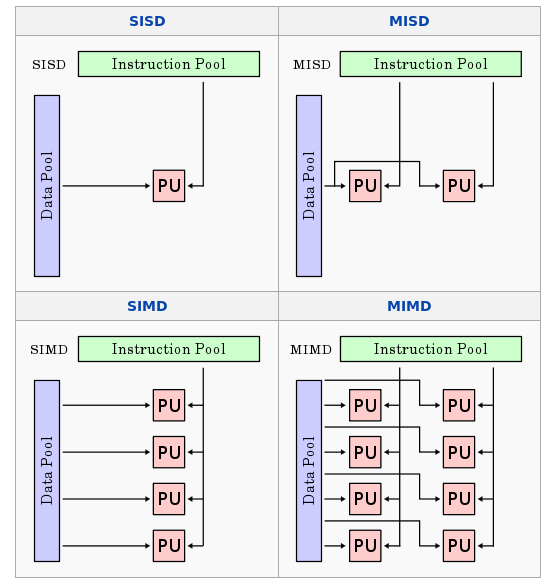
\includegraphics[width=0.80\textwidth]{figuras/flynn-ejemplo.png} \\
  \caption{Taxonom\'ia de Flynn: Comparaci\'on de las arquitecturas.} %
   \label{figFlynn1}
\end{figure}

\subsection{Modelos Paralelos}
Desde la perspectiva del sistema operativo, hay dos medios importantes de conseguir procesamiento paralelo: m\'ultiples procesos y m\'ultiples hilos. Un proceso es un programa en ejecuci\'on bajo control de un sistema operativo con un conjunto de recursos asociados. Estos recursos incluyen, pero no est\'an limitados a, estructuras de datos con informaci\'on del proceso, un espacio de direcciones virtuales conteniendo las instrucciones del programa y datos, y al menos un hilo de ejecuci\'on.  Un hilo es un camino de ejecuci\'on o flujo de control independiente dentro de un proceso, compuesto de un contexto (que incluye un conjunto de registros) y una secuencia de instrucciones a ejecutar\citep[Cap. 4]{Wad}. %OSO Hay una referencia de estas definiciones? %ANDRES est\'a sacado del libro que encontr\'e ``software optimization for high performance computing''.

En los sistemas de computaci\'on actuales existen distintos niveles de paralelismo. Por ejemplo, los procesadores VLIW y los RISC superescalares alcanzan paralelismo en el nivel de instrucci\'on (ejecutando varias instrucciones de bajo nivel al mismo tiempo)\citep{Grama, Wad}.\\
Para este trabajo de tesis utilizamos el t\'ermino ``procesamiento paralelo'' para indicar que hay m\'as de un hilo de ejecuci\'on ejecut\'andose en un \'unico programa. Esta definici\'on admite la implementaci\'on de procesamiento paralelo con m\'as de un proceso. Podemos as\'i considerar el procesamiento paralelo en tres categor\'ias\citep[Cap. 4]{Wad}:
\begin{itemize}
\item ``Paralelismo de procesos'': usar m\'as de un proceso para desempe\~nar un conjunto de tareas.
\item ``Paralelismo de hilos'': usar m\'ultiples hilos dentro de un \'unico proceso para ejecutar un conjunto de tareas.
\item ``Paralelismo h\'ibrido'': usar m\'ultiples procesos, donde al menos uno de ellos es un proceso paralelo con hilos, para desempe\~nar un conjunto de tareas.
\end{itemize}
Si bien se puede obtener paralelismo con m\'ultiples procesos, existen al menos dos razones potenciales para considerar paralelismo de hilos: conservaci\'on de recursos del sistema y ejecuci\'on m\'as r\'apida. Los hilos comparten acceso a los datos del proceso, archivos abiertos y otros atributos del proceso. Compartir datos e instrucciones puede reducir los requerimientos de recursos para un trabajo en particular. Por el contrario, una colecci\'on de procesos a menudo deber\'a duplicar las \'areas de datos e instrucciones en memoria para un trabajo.

\subsubsection{Conceptos b\'asicos de hilos}
La administraci\'on de hilos es m\'as simple que la de los procesos, ya que los hilos no poseen todos los atributos de un proceso. Pueden ser creados y destruidos mucho m\'as r\'apidamente que un proceso. Los hilos tienen otros atributos importantes, relacionados con el desempe\~no\citep[Cap. 4]{Wad}.\\

Un hilo ocioso es aquel que no tiene procesamiento para hacer y est\'a esperando su pr\'oximo conjunto de tareas. Por lo general el hilo es puesto en estado de espera (wait) de acuerdo con una variable de control, que puede tener dos valores, bloqueado o desbloqueado (debe esperar o puede continuar procesando, respectivamente).\\

Los hilos ociosos pueden ser suspendidos o quedar en espera activa (``spinning'' o ``busy waiting'')\citep[Cap. 4]{Wad}. Los hilos suspendidos liberan el procesador donde se estaban ejecutando. Los que est\'an en espera activa comprobar\'an repetidamente la variable para ver si ya est\'an desbloqueados, sin liberar el procesador para otros procesos. Como resultado de esto el rendimiento del sistema puede degradarse dr\'asticamente. Sin embargo, reiniciar un hilo suspendido puede llevar cientos, si no miles, de ciclos de procesador.\\

Otro atributo de los hilos es la afinidad, que consiste en la posibilidad de ligar un hilo con un mismo procesador al ser reiniciado luego de una suspensi\'on\citep[Cap. 4]{Wad}. La capacidad de manejar la afinidad permite mantener al hilo, siempre que sea posible, ejecutando sobre el mismo dispositivo de c\'omputo cada vez que vuelve al modo activo. De esta manera el hilo aprovecha los datos que hab\'ian sido puestos en cache durante su ejecuci\'on previa. De otro modo, deber\'ia volver a cargar todos los datos necesarios para reanudar su ejecuci\'on desde la memoria a la cache del nuevo procesador, con el costo de sobrecarga correspondiente.

\subsubsection{Hilos POSIX}
Reci\'en en 1995 se estableci\'o un est\'andar para la programaci\'on de hilos, a pesar de que los sistemas operativos ven\'ian implementando hilos desde hac\'ia d\'ecadas. El est\'andar es parte de la normativa ``POSIX (Portable Operating System Interface)'', en particular la porci\'on POSIX 1003.1c\footnote{\url{http://http://www.unix.org/version3/ieee_std.html}} incluye las funciones y las Interfaces de Programaci\'on de Aplicaci\'on (``APIs'') que soportan m\'ultiples flujos de control dentro de un proceso. Los hilos creados y manipulados v\'ia este est\'andar son generalmente indicados como ``pthreads''. Con anterioridad al establecimiento de este est\'andar, las APIs de hilos eran espec\'ificas del fabricante del hardware, lo que hac\'ia muy dificil la portabilidad de las aplicaciones paralelas con hilos. Combinado con la complejidad de reescribir aplicaciones para utilizar y aprovechar el control expl\'icito de hilos, el resultado era que muy pocas aplicaciones paralelas utilizaban el modelo de hilos\citep[Cap. 4]{Wad}.
 
\subsubsection{Paralelismo basado en directivas del compilador}
El uso de directivas del compilador para conseguir paralelismo tiene el fin de aliviar la complejidad y los problemas de la portabilidad. En el paralelismo orientado a directivas, la mayor\'ia de los mecanismos paralelos se ponen en marcha a trav\'es del compilador (generaci\'on de hilos, generaci\'on de construcciones de sincronizaci\'on, etc.). Es decir, el compilador traduce las directivas de compilador en las llamadas al sistema necesarias para la administraci\'on de los hilos, y realiza cualquier reestructuraci\'on del c\'odigo que sea necesaria. Estas directivas proveen una manera simple de lograr paralelismo.

El est\'andar ``OpenMP''\citep{openmp} para directivas de compilador paralelas ha promovido el uso de esta forma de programaci\'on paralela. Antes de la aparici\'on de este est\'andar, las directivas de compilador eran espec\'ificas del fabricante del hardware, lo que dificultaba la portabilidad. 
Tanto la implementaci\'on expl\'icita de hilos paralelos (como pthreads) como el paralelismo basado en directivas (como OpenMP) se benefician del uso de memoria compartida.

\subsubsection{Paralelismo de memoria compartida}
El paralelismo de hilos depende de la existencia de la memoria compartida para la comunicaci\'on entre hilos. Otro modelo paralelo anterior tambi\'en utiliza memoria compartida, pero entre procesos. Este paralelismo de procesos t\'ipicamente se logra a trav\'es del uso de las llamadas al sistema ``fork()'' y ``exec()''  o sus an\'alogas. Por ello se lo denomina generalmente como el modelo ``fork/exec''. La memoria es compartida entre los procesos en virtud de las llamadas al sistema ``mmap()'' (derivada de Berkeley UNIX) o ``shmget()'' (de System V UNIX)\citep{Wad}.

\subsubsection{Pasaje de Mensajes}
El modelo fork/exec no implica la existencia de memoria compartida. Los procesos pueden comunicarse a trav\'es de interfaces de E/S tales como las llamadas al sistema ``read()'' y ``write()''. Esto puede darse a trav\'es de archivos regulares o a trav\'es de alguna otra forma est\'andar de comunicaci\'on entre procesos como los ``sockets''.  La comunicaci\'on a trav\'es de archivos resulta f\'acil entre procesos que comparten un sistema de archivos, pudiendo extenderse a varios sistemas al utilizar un sistema de archivos compartido como NFS. Los sockets son usualmente un medio de comunicaci\'on m\'as eficiente entre procesos ya que eliminan gran parte del costo de realizar operaciones sobre un sistema de archivos.

Estas dos t\'ecnicas comunes dependen de que el proceso escriba, o env\'ie, el dato a ser comunicado hacia un archivo o socket. Este acto de comunicaci\'on se considera un mensaje, esto es, el proceso emisor est\'a enviando un mensaje al proceso receptor. De ah\'i el nombre de pasaje de mensajes para este modelo.

Han existido diferentes implementaciones de bibliotecas de pasaje de mensajes, como PAR-MACS (para macros paralelas) y PVM (Parallel Virtual Machine)\citep{Wad,Grama}. Luego, en 1994, surge ``MPI''\citep{mpi} en un intento de brindar una API est\'andar de pasaje de mensajes. MPI pronto desplaz\'o a PVM y fue adoptando algunas de las ventajas de \'esta. A\'un cuando fue pensada principalmente para m\'aquinas de memoria distribuida, tiene la ventaja de que puede ser aplicada tambi\'en en m\'aquinas de memoria compartida. MPI est\'a destinado a paralelismo de procesos, no paralelismo de hilos.

\subsection{Infraestructuras de hardware para paralelismo}
Hist\'oricamente, las arquitecturas de computadoras paralelas han sido muy diversas. Existen a\'un diversas arquitecturas b\'asicas disponibles comercialmente hoy en d\'ia. En las siguientes secciones se dar\'a un panorama general de las arquitecturas paralelas.

\subsubsection{Clusters}
Un cluster es una colecci\'on interconectada de equipos independientes que son utilizadas como un solo recurso de computaci\'on. Un ejemplo com\'un de cluster es simplemente un conjunto de estaciones de trabajo conectadas por una red de \'area local\citep{Wad}.

Un aspecto positivo de un cluster es que en general cada nodo est\'a de por s\'i bien balanceado en t\'erminos de procesador, sistema de memoria y capacidades de E/S (ya que cada nodo es una computadora). Otra ventaja es el costo: un cluster puede consistir de estaciones de trabajo est\'andar, de f\'acil adquisici\'on. Del mismo modo, la interconexi\'on de los nodos puede ser resuelta con tecnolog\'ias de red local est\'andar como Ethernet, FDDI, etc. Los clusters tambi\'en resultan escalables, agreg\'andose nodos al sistema paralelo simplemente agregando m\'as estaciones de trabajo.\\

La capacidad y el desempe\~no de las interconexiones son dos puntos cr\'iticos de los clusters. Las operaciones que acceden a datos residentes en el mismo nodo donde est\'a ejecut\'andose la aplicaci\'on ser\'an relativamente r\'apidas; acceder a datos residentes en otros nodos resulta algo muy diferente. Los datos remotos deber\'an ser transferidos v\'ia llamadas al sistema para pasaje de mensajes. Esto implica los costos de la sobrecarga del mecanismo de llamadas al sistema y de la latencia de las comunicaciones, que dependen de la tecnolog\'ia de la red subyacente.\\

La administraci\'on del sistema presenta otro problema. Sin software especial para esta tarea, es complejo administrar el sistema. El software debe instalarse en cada nodo individual, lo cual puede ser un proceso lento y costoso (por ejemplo, si se necesita una licencia por cada nodo).\\

Otro aspecto es la carencia de una imagen \'unica del sistema. Nos referimos a la capacidad de que el cluster deba verse como un sistema solo y no como un conjunto de computadoras. Un usuario que ingresa en el sistema puede hacerlo siempre desde la misma estaci\'on de trabajo, con lo cual no ver\'a diferencias, pero si lo realiza desde distintas estaciones puede ver un ambiente muy distinto al cambiar de equipo. Por lo general se busca mantener los archivos utilizados por el usuario disponibles cada vez que ingrese, sin importar el equipo en el que est\'e, lo que trae mayor complejidad al cluster\citep{Wad}.

\subsubsection{Multiprocesadores Sim\'etricos (SMPs)}
Las computadoras multiprocesador suponen una alternativa para evitar los problemas de los clusters. En un multiprocesador, todos los procesadores acceden a todos los recursos de la m\'aquina. Cuando los procesadores son todos iguales y cada uno tiene acceso igualitario a los recursos de la computadora, el sistema se llama Multiprocesador Sim\'etrico (SMP por la sigla en ingl\'es)\citep{Wad}.

En los sistemas con modo dual de operaci\'on, las instrucciones privilegiadas se ejecutan en modo privilegiado o kernel. El proceso, que corre en modo de usuario, logra esto mediante llamadas al sistema, lo que provoca que el sistema operativo tome control sobre el hilo de ejecuci\'on del programa por un per\'iodo de tiempo. En un sistema multiprocesador, si s\'olo una CPU a la vez puede ejecutar en modo kernel, aparece un cuello de botella que transformar\'a la computadora multiprocesador en un sistema de un solo procesador.  Un equipo SMP debe ser capaz de que todos sus procesadores ejecuten en modo kernel. 

Al proveer un solo espacio de direcciones para las aplicaciones, un sistema SMP puede hacer el desarrollo de aplicaciones m\'as f\'acil que en un sistema con m\'ultiples e independientes espacios de direcciones como un cluster.

Un sistema SMP tendr\'a m\'ultiples procesadores, pero en realidad no tiene m\'ultiples sistemas de E/S o de memoria. Ya que en los SMP se tiene acceso igual o uniforme a la memoria, se dice que son m\'aquinas de Acceso Uniforme a Memoria (UMA - Uniform Memory Access). UMA implica que todos los procesadores pueden acceder a la memoria con la misma latencia. %OSO Aclarar que los modernos multicore son NUMA debido a la cache distribuida

\subsubsection{Buses y Crossbars}
Hay diferentes tecnolog\'ias que permiten conectar los dispositivos de c\'omputo entre s\'i y con el resto de los dispositivos del sistema. Un bus puede ser visto como un conjunto de l\'ineas de conexi\'on utilizado para conectar varios perif\'ericos de la computadora. La comunicaci\'on entre los recursos f\'isicos se hace com\'unmente con un bus. Generalmente hay dos grupos de buses en un sistema: buses de E/S y de memoria. Los de E/S t\'ipicamente son largos, pueden tener diferentes tipos de dispositivos conectados y normalmente acatan un est\'andar. Por el otro lado, los buses de memoria son cortos, de alta velocidad y usualmente optimizados, para maximizar el desempe\~no conjunto entre el procesador y la memoria. 

Otro m\'etodo com\'un de interconectar dispositivos es a trav\'es de crossbars. Un crossbar se asemeja a un conjunto m\'ultiples buses independientes que conectan cada uno de los m\'odulos en el multiprocesador. La implementaci\'on de un crossbar en hardware es sumamente complicada, debido a que debe permitir tantas comunicaciones independientes como sea posible mientras arbitra los pedidos m\'ultiples de acceso a un mismo recurso, tal como un banco de memoria. Todos los posibles caminos no conflictivos deben ser permitidos simult\'aneamente, pero esto supone un desarrollo complejo del hardware\citep{Wad}.

\section{C\'omputo de Altas Prestaciones}\label{sec:n2}
Luego de revisar el concepto de la computaci\'on paralela, las formas en que se categoriza y sus distintos modelos, definimos lo que podr\'ia llamarse una consecuencia de su evoluci\'on: el c\'omputo de altas prestaciones.

Un gran problema transversal a las Ciencias e Ingenier\'ias Computacionales es la aplicaci\'on eficiente de modernas herramientas de c\'omputo paralelo y distribuido. La respuesta a este problema est\'a condensada en el concepto de Computaci\'on de Altas Prestaciones (High Performance Computing, o HPC) que abarca todos aquellos principios, m\'etodos y t\'ecnicas que permiten abordar problemas con estructuras de c\'omputo complejas y de altos requerimientos.

El objetivo del proyecto HPC en la FaI es adquirir conocimientos para el dise\~no, desarrollo, gesti\'on y mejora de las tecnolog\'ias de hardware y software involucradas en la Computaci\'on de Altas Prestaciones (CAP) y sus aplicaciones en Ciencias e Ingenier\'ia Computacional.

Tradicionalmente, el \'ambito donde surg\'ian los productos de la ciencia y de la ingenier\'ia eran los laboratorios. Combinando la teor\'ia y la experimentaci\'on, con c\'alculos hechos a mano o apoy\'andose en herramientas de c\'alculo rudimentarias, se aplicaba el conocimiento de la f\'isica, la matem\'atica, la biolog\'ia, para obtener y validar nuevos conocimientos. La aparici\'on de las computadoras ofreci\'o una nueva y potente forma de hacer ciencia e ingenier\'ia: la ejecuci\'on de programas que utilizan modelos matem\'aticos y soluciones num\'ericas para resolver los problemas.

As\'i surgen herramientas como la simulaci\'on num\'erica, proceso de modelar matem\'aticamente un fen\'omeno de la realidad, y ejecutar experimentos virtuales a partir del modelo implementado en computador. En cada disciplina podemos encontrar experimentos que, por ser de alto costo, complejos, peligrosos o simplemente impracticables, hacen de la simulaci\'on num\'erica una herramienta de enorme valor. De la misma manera, las computadoras permiten la obtenci\'on de resultados concretos para problemas de c\'alculo imposibles de abordar en forma manual.

\subsection{Ciencia e Ingenier\'ia Computacional}
La situaci\'on descripta en  los p\'arrafos anteriores ha dado auge a un nuevo campo interdisciplinario denominado Ciencia e Ingenier\'ia Computacional (Computational Science \& Engineering, CSE), que es la intersecci\'on de tres dominios: matem\'atica, ciencias de la computaci\'on, y las diferentes ramas de las ciencias o ingenier\'ias. La Ciencia e Ingenier\'ia Computacional usa herramientas de las ciencias de la computaci\'on y las matem\'aticas para estudiar problemas de las ciencias f\'isicas, sociales, de la Tierra, de la vida, de las diferentes disciplinas ingenieriles, etc.

Durante la presente d\'ecada, la Ciencia e Ingenier\'ia Computacional ha visto un desarrollo espectacular. Puede decirse que las tecnolog\'ias de c\'omputo y de comunicaciones han modificado el campo cient\'ifico de una manera que no admite el retroceso, sino que, al contrario, la superaci\'on y extensi\'on de esas tecnolog\'ias resulta vital para poder seguir haciendo ciencias como las conocemos hoy.

Gracias a estos avances tecnol\'ogicos los cient\'ificos pueden trascender sus anteriores alcances, extender sus resultados y abordar nuevos problemas, antes intratables. Entre los m\'etodos de la Ciencia e Ingenier\'ia Computacional se incluyen:

\begin{itemize}
\item Simulaciones num\'ericas, con diferentes objetivos:
     \begin{itemize}
      \item Reconstrucci\'on y comprensi\'on los eventos naturales conocidos: terremotos, incendios forestales, maremotos, etc.
      \item Predicci\'on del futuro o de situaciones inobservables: predicci\'on del tiempo, comportamiento de part\'iculas subat\'omicas.
     \end{itemize}
\end{itemize} 
\begin{itemize}
\item Ajustes de modelos y an\'alisis de datos
      \begin{itemize}
      \item Sintonizaci\'on de modelos o resoluci\'on de ecuaciones para reflejar observaciones, sujetas a las limitaciones del modelo: prospecci\'on geof\'isica, lingü\'istica computacional.
      \item Modelado de redes, en particular aquellas que conectan individuos, organizaciones, o sitios web.
      \item Procesamiento de im\'agenes, inferencia de conceptos y discriminantes: detecci\'on de caracter\'isticas del terreno, de procesos climatol\'ogicos, reconocimiento de patrones gr\'aficos
      \end{itemize}
\end{itemize}
\begin{itemize}
\item Optimizaci\'on
      \begin{itemize}
      \item An\'alisis y mejoramiento de escenarios conocidos, como procesos t\'ecnicos y de manufactura.
      \end{itemize}
\end{itemize}
A estos m\'etodos, cuya aplicaci\'on hoy ya es corriente en las ciencias e ingenier\'ias, se suman ciertos problemas, denominados ``grandes desaf\'ios'', y cuya soluci\'on tiene amplio impacto sobre el desarrollo de esas disciplinas. Estos problemas pueden ser tratados por la aplicaci\'on de t\'ecnicas y recursos de Computaci\'on de Altas Prestaciones. Algunos de los campos donde aparecen estos problemas son:

\begin{itemize}
\item Din\'amica de fluidos computacional, para el dise\~no de aeronaves, la predicci\'on del tiempo a t\'erminos cortos o largos, para la recuperaci\'on eficiente de minerales, y muchas otras aplicaciones.
\item C\'alculos de estructuras electr\'onicas, para el dise\~no de nuevos materiales como catal\'iticos qu\'imicos, agentes inmunol\'ogicos, o superconductores.
\item C\'omputos que permitan comprender la naturaleza fundamental de la materia y de los procesos de la vida.
\item Procesamiento simb\'olico, incluyendo reconocimiento del habla, visi\'on por computadora, comprensi\'on del lenguaje natural, razonamiento automatizado y herramientas varias para dise\~no, manufactura y simulaci\'on de sistemas complejos.
\end{itemize}
La resoluci\'on de estos problemas involucra conjuntos masivos de datos, una gran cantidad de variables y complejos procesos de c\'alculo; por otro lado, es de car\'acter abierto, en el sentido de que siempre aparecer\'an escenarios de mayor porte o mayor complejidad para cada problema. Estos m\'etodos y sus t\'ecnicas particulares exigen la utilizaci\'on de recursos de computaci\'on hasta hoy excepcionales, como lo han sido las supercomputadoras, los multiprocesadores y la colaboraci\'on de una gran cantidad de computadoras a trav\'es de las redes, en diferentes niveles de agregaci\'on como clusters, multiclusters y grids.

\section{Fortran}\label{sec:n3}
Muy popular en la programaci\'on cient\'ifica y la computaci\'on de alto desempe\~no (HPC), el lenguaje Fortran surge a mediados de la d\'ecada de 1950, siendo uno de los lenguajes de programaci\'on m\'as antiguos utilizados a\'un hoy por cient\'ificos de todo el mundo. Se lo clasifica como un lenguaje de programaci\'on de alto nivel (considerado el primero de ellos en aparecer), de prop\'osito general e imperativo. La programaci\'on imperativa describe un programa en t\'erminos del estado del programa y las sentencias que cambian dicho estado, como descripto por una m\'aquina de Turing.  

Fue desarrollado para aplicaciones cient\'ificas y de ingenier\'ia, campos que domin\'o r\'apidamente, siendo durante todo este tiempo ampliamente utilizado en \'areas de c\'omputo intensivo, tales como el an\'alisis de elementos finitos, predicci\'on num\'erica del clima, din\'amica de fluidos computacional o f\'isica computacional. 
Ampliamente adoptado por cient\'ificos para escribir programas num\'ericamente intensivos, impuls\'o a los constructores de compiladores a generar c\'odigo m\'as r\'apido y eficiente. La inclusi\'on de un tipo de dato complejo (COMPLEX) lo hizo especialmente apto para aplicaciones t\'ecnicas como la Ingenier\'ia El\'ectrica. 

En las \'areas cient\'ificas, con t\'ipicos problemas de c\'alculo intensivo, una vez que un programa alcanza un estado de computaci\'on correcta (i.e. arroja los resultados deseados), no suelen ocurrir modificaciones del c\'odigo. En el caso de Fortran, su adopci\'on por la comunidad cient\'ifica deriv\'o en la construcci\'on de programas que permanecen vigentes tras 20, 30 y hasta 40 a\~nos. Estos constituyen lo que denominamos ``Legacy Software''. Se ha definido al Legacy Software como:

\begin{itemize}
\item ``Software cr\'itico que no puede ser modificado eficientemente''\citep{Gold}.
\item ``Cualquier sistema de informaci\'on que significativamente resiste las modificaciones y la evoluci\'on para alcanzar requerimientos de negocio nuevos y constantemente cambiantes''\citep{Brod}. 
\end{itemize}
Algunas caracter\'isticas de los sistemas legacy son:

\begin{itemize}
\item La resistencia al cambio del software.
\item La complejidad inherente.
\item La tarea crucial desempe\~nada por el software en la organizaci\'on.
\item El tama\~no del sistema, generalmente mediano o grande.
\end{itemize}
Es com\'un hallar software hecho en Fortran que ha estado ejecut\'andose en ambientes de producci\'on por d\'ecadas. Durante ese per\'iodo, el software se deteriora gradualmente y puede necesitar cambios de diferente tipo, como: mejoras, correcciones, adaptaciones y prevenciones. Para todas estas tareas se necesita conocimiento y comprensi\'on del sistema. En la era multi-core y many-core, los cambios de software se hacen m\'as y m\'as complejos\citep{MMen}.
%OSO Est\'a bien esta frase?. la siguiente- cita a donde es nombrada
Debido a que Fortran ha estado tantos a\~nos vigente, ha pasado por un proceso particular de estandarizaci\'on en el cual cada versi\'on previa del est\'andar cumple con el vigente. Este proceso de estandarizaci\'on permite que un programa en Fortran 77 compile en los compiladores modernos de Fortran 2008\citep{MMen}. Gracias a estas caracter\'isticas es que el lenguaje est\'a, a\'un hoy y a pesar de ser relativamente poco visible, en una posici\'on s\'olida y bien definida. Actualmente hay un gran conjunto de programas Fortran ejecut\'andose en ambientes productivos de universidades, empresas e instituciones de gobierno. Algunos buenos ejemplos son programas de modelo clim\'atico, simulaciones de terremotos, simulaciones magnetohidrodin\'amicas, etc. La mayor\'ia de estos programas han sido construidos a\~nos o d\'ecadas atr\'as y sus usuarios necesitan que sean modernizados, mejorados y/o actualizados. Esto tambi\'en implica que estos programas sean capaces de aprovechar las arquitecturas de procesadores modernas y, espec\'ificamente, el equipamiento para procesamiento num\'erico.

\subsection{Evoluci\'on del lenguaje}
Fortran ha evolucionado de una release inicial con 32 sentencias para la IBM 704, entre los que estaban el condicional IF y el IF aritm\'etico de 3 v\'ias, el salto GO TO, el bucle DO, comandos para E/S tanto formateada como sin formato (FORMAT, READ, WRITE, PRINT, READ TAPE, READ DRUM, etc), y de control del programa (PAUSE, STOP, CONTINUE), y tipos de datos todos num\'ericos, hasta llegar al \'ultimo estandar Fortran, ISO/IEC 1539-1:2010, conocido informalmente como Fortran 2008, donde fueron incorpor\'andose caracter\'isticas como tipos de datos CHARACTER, definici\'on de arrays, subrutinas, funciones, recursividad, modularidad, hasta nuevas sentencias que soportan la ejecuci\'on de alta performance como DO CONCURRENT, coarrays (un modelo de ejecuci\'on paralela). Si se desea ahondar en la definici\'on del est\'andar Fortran el mismo puede encontrarse en el sitio de NAG (The Numerical Algorithms Group) quienes alojan el home oficial para los est\'andares de Fortran\footnote{\url{http://www.nag.co.uk/sc22wg5/}}.

El lenguaje utilizado en el programa de estudio de este trabajo de tesis est\'a basado en el est\'andar Fortran 77, aunque presenta libertades presentes en Fortran 90, como la utilizaci�n de minusculas indiferentemente y el formato libre de escritura. Esto es posible gracias a, como explicamos en la secci�n previa, que cada versi�n nueva del compilador soporta los est�ndares previos. Se presentan en el anexo A las sentencias de Fortran m\'as utilizadas en la aplicaci\'on objeto de estudio.

\section{OpenMP}\label{sec:n4}
OpenMP es una Interfaz de Programaci\'on de Aplicaciones, o API por sus siglas en Ingles, la cual provee un modelo portable y escalable para el desarrollo de aplicaciones paralelas de memoria compartida. La API soporta C/C++ y Fortran en una gran variedad de arquitecturas. Es utilizada para de manera directa aplicar multihilos en memoria compartida\footnote{\url{https://computing.llnl.gov/tutorials/openMP/}}.

La especificaci\'on de OpenMP\citep{openmp} pertenece, es escrita y mantenida por la OpenMP Architecture Review Board, que es la uni\'on de las compa\~n\'ias que tienen participaci\'on activa en el desarrollo del est\'andar para la interfaz de programaci\'on en memoria compartida\citep{Her}.

No es un nuevo lenguaje de programaci\'on, sino que es una notaci\'on que puede ser agregada a un programa secuencial en Fortran, C o C++ para describir como el trabajo debe ser compartido entre los hilos que se ejecutaran en diferentes procesadores o n\'ucleos y para organizar el acceso a los datos compartidos cuando sea necesario.
La inserci\'on apropiada de las caracter\'isticas de OpenMP en un programa secuencial permitir\'a a muchas, si no a la mayor\'ia, de las aplicaciones beneficiarse de una arquitectura de memoria compartida, a menudo con m\'inimas modificaciones al c\'odigo.
Uno de los factores del \'exito de OpenMP es que es comparativamente sencillo de usar, ya que el trabajo m\'as complicado de armar los detalles del programa paralelo son dejados para el compilador. Tiene adem\'as la gran ventaja de ser ampliamente adoptado, de manera que una aplicaci\'on OpenMP va a poder ejecutarse en muchas plataformas diferentes\citep[Cap. 1]{Chap}.

Las directivas de OpenMP permiten al usuario indicarle al compilador que instrucciones ejecutar en paralelo y como distribuir las mismas entre los hilos que van a ejecutar el c\'odigo.
Una de estas directivas es una instrucci\'on en un formato especial que es entendido por compiladores OpenMP solamente. De hecho luce como un comentario para un compilador Fortran regular, o una diretiva pragma para un compilador C/C++, de manera que el programa puede ejecutarse como lo hac\'ia previamente si el compilador no conoce OpenMP.
Generalmente se puede r\'apida y f\'acilmente crear programas paralelos confiando en la implementaci\'on para que trabaje los detalles de la ejecuci\'on paralela. Pero no siempre es posible obtener alta performance con una inserci\'on sencilla, incremental de directivas OpenMP en un c\'odigo secuencial. Por esta raz\'on OpenMP incluye varias caracter\'isticas que habilitan al programador a especificar m\'as detalle en el c\'odigo paralelo.

\subsection{La idea de OpenMP}
Un hilo es una entidad en tiempo de ejecuci\'on que es capaz de ejecutar independientemente un flujo de instrucciones. OpenMP trabaja en un cuerpo m\'as grande de trabajo que soporta la especificaci\'on de programas para ser ejecutados por una colecci\'on de hilos cooperativos. El sistema operativo crea un proceso para ejecutar un programa: reservar\'a algunos recursos para este proceso, incluyendo p\'aginas de memoria y registros para almacenar valores de objetos. Si multiples hilos colaboran para ejecutar un programan, compartir\'an los recursos, incluyendo el espacio de direcciones, del correspondiente proceso. Los hilos individuales necesitan muy pocos recursos por si mismos: un contador de programa y un \'area de memoria para guardar variables especificas del hilo (incluyendo registros y una pila)\citep[Cap. 2]{Chap}.
OpenMP intenta proveer facilidad de programaci\'on y ayudar al usuario a evitar un n\'umero de potenciales errores de programaci\'on, ofreciendo un enfoque estructurado para la programaci\'on multihilo. Soporta el modelo de programaci\'on llamado fork-join, el cual podemos ver en la Fig. \ref{figFork1}.

\begin{figure}[h!]%[htp]
  \centering
  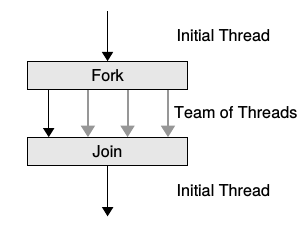
\includegraphics[width=0.50\textwidth]{figuras/fork-join1.png} \\
  \caption{Modelo fork-join} %
   \label{figFork1}
\end{figure}

Bajo este enfoque, el programa inicia como un solo hilo de ejecuci\'on (denominado hilo inicial), igual que un programa secuencial. Siempre que se encuentre una construcci\'on paralela de OpenMP por el hilo mientras ejecuta su programa, se crea un equipo de hilos (esta es la parte fork), se convierte en el maestro del equipo, y colabora con los otros miembros del equipo para ejecutar el c\'odigo din\'amicamente encerrado por la construcci\'on. Al final de la construcci\'on, solo el hilo original, o maestro del equipo, continua; todos los dem\'as terminan (esta es la parte join). Cada porci\'on del c\'odigo encerrada por una construcci\'on paralela es llamada una regi\'on paralela.

\subsection{Conjunto de construcciones paralelas}
La API OpenMP comprende un conjunto de directivas del compilador, rutinas de bibliotecas de tiempo de ejecuci\'on, y variables de ambiente para especificar paralelismo de memoria compartida. Muchas de las directivas son aplicadas a un bloque estructurado de c\'odigo, una secuencia de sentencias ejecutables con una sola entrada en la parte superior y una sola salida en la parte inferior en los programas Fortran, y una sentencia ejecutable en C/C++ (que puede ser una composici\'on de sentencias con una sola entrada y una sola salida). En otras palabras, el programa no puede ramificarse dentro o fuera de los bloques de c\'odigo asociados con directivas. En Fortran el inicio y el final del bloque aplicable de c\'odigo son marcados expl\'icitamente por una directiva OpenMP\citep[Cap. 2]{Chap}.

\subsubsection{Crear equipos de Hilos}
Un equipo de hilos es creado para ejecutar el c\'odigo en una regi\'on paralela de un programa OpenMP. El programador simplemente especifica la regi\'on paralela insertando una directiva \emph{parallel} inmediatamente antes del c\'odigo que debe ser ejecutado en paralelo para marcar su inicio; en los programas Fortran el final tambi\'en es indicado por una directiva end parallel. Informaci\'on adicional puede ser provista junto con la diretiva \emph{parallel}, como habilitar a los hilos a tener copias privadas de alg\'un dato por la duraci\'on de la regi\'on paralela. El final de una regi\'on paralela es una barrera de sincronizaci\'on impl\'icita: esto significa que ning\'un hilo puede progresar hasta que todos los dem\'as hilos del equipo hayan alcanzado este punto del programa\citep[Cap. 2]{Chap}. Es posible realizar anidado de regiones paralelas.

\subsubsection{Compartir trabajo entre Hilos}
Si el programador no especifica como se compartir\'a el trabajo en una regi\'on paralela, todos los hilos ejecutar\'an el c\'odigo completo redundantemente, sin mejorar los tiempos del programa. Para ello OpenMP cuenta con directivas para compartir trabajo que permiten indicar como se distribuir\'a el computo en un bloque de c\'odigo estructurado entre los hilos. A menos que el programador lo indique expl\'icitamente, una barrera de sincronizaci\'on existe impl\'icitamente al final de las construcciones de trabajo compartido\citep[Cap. 2]{Chap}.

Probablemente el m\'etodo m\'as com\'un de trabajo compartido es distribuir el trabajo en un bucle DO (Fortran) o for (C/C++) entre los distintos hilos de un equipo. El programador inserta la directiva apropiada inmediatamente antes de los bucles que vayan a ser compartidos entre los hilos dentro de una regi\'on paralela.
Todas las estrategias de OpenMP para compartir el trabajo en un bucle asignan uno o m\'as conjuntos disjuntos de iteraciones a cada hilo. El programador puede, si as\'i lo desea, especificar el m\'etodo para particionar el conjunto de iteraci\'on.

\subsubsection{Modelo de memoria de OpenMP}
OpenMP se basa en el modelo de memoria compartida, por ello, por defecto los datos son compartidos por todos los hilos y son visibles para todos. A veces es necesario tener variables que tienen valores espec\'ificos por hilo. Cuando cada hilo tiene una copia propia de una variable, donde potencialmente tenga valores distintos en cada uno de ellos, decimos que la variable es privada. Por ejemplo, cuando un equipo de hilos ejecuta un bucle paralelo  cada hilo necesita su propio valor de la variable de control de iteraci\'on. Este caso es tan importante que el propio compilador fuerza que as\'i sea; en otros casos el programador es quien debe determinar cuales variables son compartidas y cuales privadas\citep[Cap. 2]{Chap}.

\subsubsection{Sincronizaci\'on de Hilos}
Sincronizar los hilos es necesario en ocasiones para asegurar el acceso en orden a los datos compartidos y prevenir corrupci\'on de datos. Asegurar la coordinaci\'on de hilos necesaria es uno de los desaf\'ios m\'as fuertes de la programaci\'on de memoria compartida\citep[Cap. 2]{Chap}. OpenMP provee, por defecto, sincronizaci\'on impl\'icita haciendo que los hilos esperen al final de una construcci\'on de trabajo compartido o regi\'on paralela hasta que todos los hilos en el equipo terminan su porci\'on de trabajo. M\'as dif\'icil de conseguir en OpenMP es coordinar las acciones de un subconjunto de los hilos ya que no hay soporte expl\'icito para esto.
Otras veces es necesario asegurar que solo un hilo a la vez trabaja en un bloque de c\'odigo. OpenMP  tiene varios mecanismos que soportan este tipo de sincronizaci\'on.

\subsubsection{Otras caracteristicas}
Subrutinas y funciones pueden complicar la utilizaci\'on de APIs de Programaci\'on Paralela. Una de las caracter\'isticas innovativas de OpenMP es el hecho de que las directivas pueden ser insertadas dentro de procedimientos que son invocados desde dentro de una regi\'on paralela.\\
Para algunas aplicaciones puede ser necesario controlar el n\'umero de hilos que ejecutan la regi\'on paralela. OpenMP permite al programador especificar este n\'umero previo a la ejecuci\'on del programa a trav\'es de una variable de ambiente, luego de que el c\'omputo a iniciado a trav\'es de una librer\'ia de rutinas, o al comienzo de regiones paralelas. Si no se hace esto, la implementaci\'on de OpenMP utilizada elegir\'a el n\'umero de hilos a utilizar\citep[Cap. 2]{Chap}.

\section{OpenMP en Fortran}\label{sec:n5}
Fueron presentados Fotran y OpenMP, en esta secci\'on se ve como se complementan, mostrando cuales es el formato de las directivas de OpenMP en Fortran.

\subsection{Centinelas para directivas de OpenMP y compilaci\'on condicional}

El est\'andar OpenMP ofrece la posibilidad de usar el mismo c\'odigo fuente con un compilador que implementa OpenMP como con uno normal. Para ello debe ocultar las directivas y comandos de una manera que un compilador normal no pueda verlas. Para ello existen las siguientes directivas centinelas\citep{Her}
\begin{lstlisting}[style=For, numbers=none]
 !$OMP

 !$
\end{lstlisting}
Como el primer caracter es un signo de exclamaci\'on ``!'', un compilador normal va a interpretar las l\'ineas como comentarios y va a ignorar su contenido. Pero un compilador compatible con OpenMP identificar\'a la sentencia y proceder\'a como sigue\citep{Her}
\begin{itemize}
\item !\$OMP : el compilador compatible con OpenMP sabe que la informaci\'on que sigue en la l\'inea es una directiva OpenMP. Se puede extender una directiva en varias l\'ineas utilizando el mismo centinela frente a las siguientes l\'ineas y usando el m\'etodo est\'andar de Fortran para partir l\'ineas de c\'odigo:
   \begin{lstlisting}[style=For, numbers=none]
        !$OMP PARALLEL DEFAULT(NONE) SHARED(A, B) &
        !$OMP REDUCTION(+:A)
   \end{lstlisting}
\end{itemize}
Es obligatorio incluir un espacio en blanco entre la directiva centinela y la directiva OpenMP que le sigue, sino la l\'inea ser\'a interpretada como un comentario.
\begin{itemize}
\item !\$ : la l\'inea correspondiente se dice que est\'a afectada por una compilaci\'on condicional. Quiere decir que su contenido estar\'a disponible para el compilador en caso de que sea compatible con OpenMP. Si esto ocurre, los dos caracteres del centinela son reemplazados por dos espacios en blanco para que el compilador tenga en cuenta la l\'inea. Como en el caso anterior podemos extender la l\'inea en varias l\'ineas como sigue:
   \begin{lstlisting}[style=For, numbers=none]
	!$ interval = L * OMP_get_thread_num() / &
	!$                       (OMP_get_num_threads() - 1)
   \end{lstlisting}
\end{itemize}
Nuevamente el espacio en blanco es obligatorio entre la directiva de compilaci\'on condicional y el c\'odigo fuente que le sigue.

\subsection{El constructor de regi\'on paralela}
La directiva m\'as importante en OpenMP es la que define las llamadas regiones paralelas. Para entender mejor qu\'e es la regi\'on paralela se puede observar una representaci\'on en la Fig. \ref{figRegpar} tomada de \citep{Her}.\\
Podemos definir sencillamente que cuando se crea la regi\'on paralela se crean los hilos que ejecutaran paralelamente el c\'odigo que est\'e definido dentro de la misma.

\begin{figure}[h!]%[htp]
  \centering
  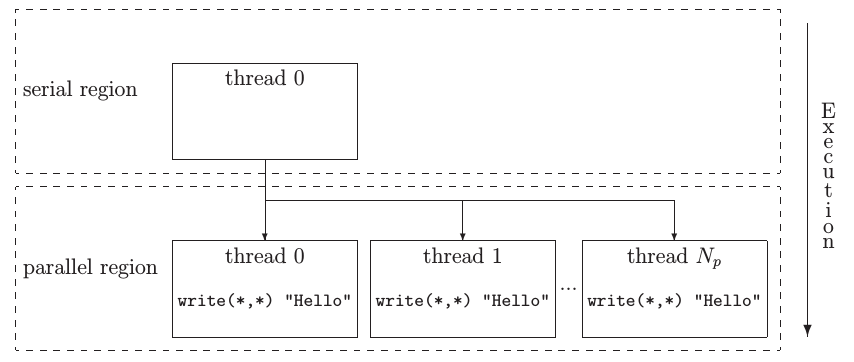
\includegraphics[width=0.80\textwidth]{figuras/reg-paralela1.png} \\
  \caption{Representaci\'on de la Regi\'on Paralela.} %
  \label{figRegpar}
\end{figure}

Ya que la regi\'on paralela necesita ser creada/abierta y destruida/cerrada, dos directivas son necesarias en Fotran: !\$OMP PARALLEL / !\$OMP END PARALLEL.
El c\'odigo de la Fig. \ref{figRegpar} se puede ver a continuaci\'on:

\begin{lstlisting}[style=For, numbers=none]
!$OMP PARALLEL 
	  write(*,*) ``Hola''
!$OMP END PARALLEL
\end{lstlisting}

Como el c\'odigo entre las dos directivas es ejecutado por cada hilo, el mensaje \emph{Hola} aparece en la pantalla tantas veces como hilos est\'en siendo usados en la regi\'on paralela.
Al comienzo de la regi\'on paralela es posible imponer cl\'ausulas que fijan ciertos aspectos de la manera en que la regi\'on paralela va a trabajar, por ejemplo el alcance de las variables, el n\'umero de hilos, etc. La sintaxis a usar es la siguiente:
\begin{lstlisting}[style=For, numbers=none]
	!$OMP PARALLEL  clause1 clause2 ...
	...
	!\$OMP END PARALLEL
\end{lstlisting}
Las cl\'ausulas permitidas en la directiva de apertura !\$OMP PARALLEL son las siguientes:
\begin{itemize}
\item PRIVATE(lista)
\item SHARED(lista)
\item DEFAULT( PRIVATE | SHARED | NONE )
\item FIRSTPRIVATE(lista)
\item COPYIN(lista)
\item REDUCTION(operador:lista)
\item IF(expresi\'on\_escalar\_l\'ogica)
\item NUM\_THREADS(expresi\'on\_escalar\_entera)
\end{itemize}
La directiva !\$OMP END PARALLEL indica el final de la regi\'on paralela, la barrera impl\'icita mencionada antes en el capitulo. En este punto es donde ocurre la sincronizaci\'on entre el equipo de hilos y son terminados todos excepto el hilo maestro que continua con la ejecuci\'on del programa.

\subsection{Directiva !\$OMP DO}
Es una directiva de trabajo compartido, por lo cual al encontrarla en el c\'odigo el trabajo es distribuido en un equipo de hilos. Debe ser ubicada dentro del alcance de una regi\'on paralela para ser efectiva, si no, la directiva a\'un funcionar\'a pero el equipo ser\'a de un solo hilo. Esto se debe a que la creaci\'on de nuevos hilos es una tarea reservada a la directiva de creaci\'on de la regi\'on paralela.
Esta directiva hace que el bucle \emph{Do} inmediato sea ejecutado en paralelo.
Por ejemplo:
\begin{lstlisting}[style=For, numbers=none]
	!$OMP DO
		do 1   i = 1, 1000
		...
	  1 continue
	!$OMP END DO
\end{lstlisting}
distribuye el bucle \emph{Do} entre los diferentes hilos, cada hilo computa una parte de las iteraciones.
Por ejemplo si usamos 10 hilos, entonces generalmente cada hilo computa 100 iteraciones del bucle do. El hilo 0 desde 1 a 100, el hilo 1 desde 101 a 200 y as\'i sucesivamente. Podemos ver esto en la Fig. \ref{figRegparDo} tomada de \citep{Her}.

\begin{figure}[h!]%[htp]
  \centering
  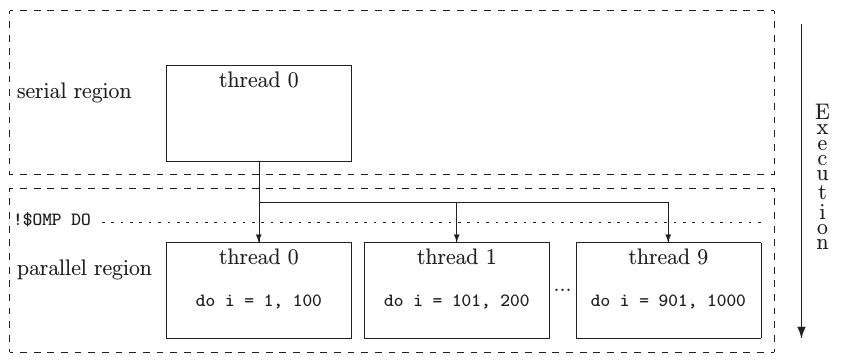
\includegraphics[width=0.80\textwidth]{figuras/reg-paralelaDo.png} \\
  \caption{Representaci\'on gr\'afica de la directiva \emph{OMP DO}.} %
  \label{figRegparDo}
\end{figure}

Dentro del trabajo de esta tesis es la directiva principal al tratarse los bucles \emph{Do} de una de las principales construcciones utilizadas en el programa estudiado.

La directiva !\$OMP DO tiene asociadas cl\'ausulas al igual que la directiva parallel, que permiten indicar el comportamiento de la construcci\'on de trabajo compartido. La sintaxis es similar:
\begin{lstlisting}[style=For, numbers=none]
	!$OMP DO clause1 clause2 ...
	...
	!$OMP END DO end_clause
\end{lstlisting}
Las cl\'ausulas de inicio pueden ser cualquiera de las siguientes:
\begin{itemize}
\item PRIVATE(lista)
\item FIRSTPRIVATE(lista)
\item LASTPRIVATE(lista)
\item REDUCTION(operador:lista)
\item SCHEDULE(tipo, pedazo)
\item ORDERED
\end{itemize}
Adicionalmente a estas cl\'ausulas de inicio, se puede agregar a la directiva de cierre la cl\'ausula NOWAIT para evitar la sincronizaci\'on impl\'icita. Tambi\'en se evita el refresco de las variables compartidas, impl\'icito en la directiva de cierre, por lo que se debe tener cuidado de cuando utilizar la cl\'ausula NOWAIT. Se pueden evitar problemas con la directiva de OpenMP !\$OMP FLUSH que fuerza el refresco de las variables compartidas en memoria por los hilos.

\subsection{Clausulas Atributo de Alcance de Datos}
\subsubsection{PRIVATE(lista)}
A veces, ciertas variables van a tener valores diferentes en cada hilo. Esto s\'olo es posible si cada hilo tiene su propia copia de la variable. Esta cl\'ausula fija que variables van a ser consideradas variables locales de cada hilo. Por ejemplo, para indicar que las variables a y b tendr\'an diferentes valores en cada hilo, i.e., ser\'an locales/privadas a cada hilo, utilizamos el siguiente c\'odigo: 

\begin{lstlisting}[style=For, numbers=none]
    !$OMP PARALLEL PRIVATE(a, b)
\end{lstlisting}

%\begin{figure}[h!]%[htp][style=For, numbers=none]
%  \centering
%    \begin{lstlisting}[style=For, numbers=none]
%        		!$OMP PARALLEL PRIVATE(a, b)
%    \end{lstlisting}
%  \caption{Ejemplo cl\'ausula PRIVATE.} %
%  \label{figPriv1}
%\end{figure}

Cuando una variable se declara como privada, un nuevo objeto del mismo tipo es declarado por cada hilo del equipo y usado por cada hilo dentro del alcance de la directiva que lo declare (la regi\'on paralela en el ejemplo anterior) en lugar de la variable original. El c\'odigo anterior se representa en la Fig. \ref{figRegparPriv} tomada de \citep{Her}.

\begin{figure}[h!]%[htp]
  \centering
  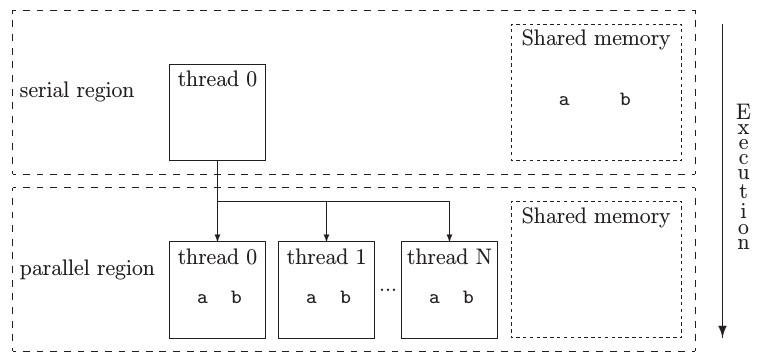
\includegraphics[width=0.80\textwidth]{figuras/reg-paralelaPriv.png} \\
  \caption{Representaci\'on gr\'afica de la cl\'ausula PRIVATE.} %
  \label{figRegparPriv}
\end{figure}

El hecho de que un nuevo objeto es creado por cada hilo puede ser algo que genere mucho consumo de recursos. Por ejemplo, si se utiliza un array de 5Gb (algo com\'un en simulaciones num\'ericas directas y otras) y es declarado como privado en una regi\'on paralela con un equipo de 10 hilos, entonces el requerimiento de memoria ser\'a de 55Gb, algo no disponible en todas las maquinas SMP.

Las variables utilizadas como contadores en los bucles \emph{Do} o comandos \emph{forall}, o son declaradas THREADPRIVATE, se convierten autom\'aticamente en privadas para cada hilo, a\'un cuando no hayan sido declaradas en un cl\'ausula PRIVATE.

\subsubsection{SHARED(lista)}

Contrario a lo visto en la situaci\'on previa, a veces hay variables que deben estar disponibles para todos los hilos dentro del alcance de una directiva, debido a que su valor es necesario para todos los hilos o porque todos los hilos deben actualizar su valor. Por ejemplo:
\begin{lstlisting}[style=For, numbers=none]
      !$OMP PARALLEL SHARED(c, d)
\end{lstlisting}
\noindent indica que las variables c y d son vistas por todos los hilos en el alcance de las directivas !\$OMP PARALLEL / !\$OMP END PARALLEL. Podemos observar en la Fig. \ref{figRegparShar} tomada de \citep{Her}, la representaci\'on deL ejemplo.

\begin{figure}[h!]%[htp]
  \centering
  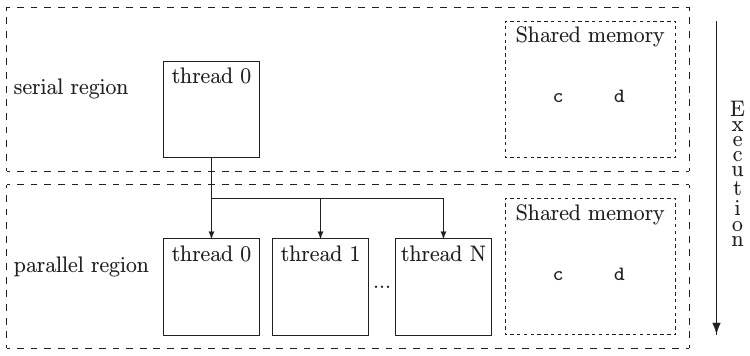
\includegraphics[width=0.80\textwidth]{figuras/reg-paralelaShar.png} \\
  \caption{Representaci\'on gr\'afica de la cl\'ausula SHARED.} %
  \label{figRegparShar}
\end{figure}

Una variable declarada como compartida (shared) no consume recursos extras, ya que no se reserva nueva memoria y su valor antes de la directiva inicial es conservado. Es decir que todos los hilos acceden a la misma ubicaci\'on de memoria para leer y escribir la variable.
Debido a que m\'as de un hilo puede escribir en la misma ubicaci\'on de memoria al mismo tiempo, resulta en un valor indefinido de la variable. A esto se lo llama una condici\'on de carrera, y debe ser siempre evitado por el programador. 

\subsubsection{DEFAULT ( PRIVATE \textbar SHARED \textbar NONE )}
Cuando la mayor\'ia de las variables dentro del alcance de una directiva va a ser privada o compartida, entonces ser\'ia engorroso incluir todas ellas en una de las cl\'ausulas previas. Para evitar esto, es posible especificar que har\'a OpenMP cuando no se especifica nada sobre una variable, es posible especificar un comportamiento por defecto. Por ejemplo:
\begin{lstlisting}[style=For, numbers=none]
      !\$OMP PARALLEL DEFAULT(PRIVATE) SHARED(a)
\end{lstlisting}
\noindent indica que todas las variables excepto ``a'' van a ser privadas, mientras que ``a'' ser\'a compartida por todos los hilos dentro del alcance de la regi\'on paralela. Si no se especifica ninguna cl\'ausula DEFAULT, el comportamiento por defecto es como si DEFAULT(SHARED) fuera especificado. Como veremos en el capitulo 3 de este trabajo de tesis, esto puede variar en implementaciones y debe ser investigado m\'as a fondo.
A las opciones PRIVATE y SHARED se le agrega una tercera: NONE. Especificando DEFAULT(NONE) requiere que cada variable en el alcance de la directiva debe ser expl\'icitamente listada en una de las cl\'ausulas PRIVATE o SHARED al principio del alcance de la directiva (exceptuando variables declaradas THREADPRIVATE o los contadores de los bucles).

\subsubsection{FIRSTPRIVATE(lista)}
Como mencionamos previamente, las variables privadas tienen un valor indefinido al comienzo del alcance de un par de directivas de inicio y cierre. Pero a veces es de inter\'es que esas variables locales tengan el valor de la variable original antes de la directiva de inicio. Esto se consigue incluyendo la variable en una cl\'ausula FIRSTPRIVATE como:
\begin{lstlisting}[style=For, numbers=none]
	a = 2
	b = 1
	!$OMP PARALLEL PRIVATE(a) FIRSTPRIVATE(b)
\end{lstlisting}
En este ejemplo, la variable ``a'' tiene un valor indefinido al inicio de la regi\'on paralela, mientras que ``b'' tiene el valor especificado en la regi\'on serial precedente, es decir ``b = 1''. Podemos ver este ejemplo en la Fig. \ref{figRegparVarPriv} tomada de \citep{Her}.

\begin{figure}[h!]%[htp]
  \centering
  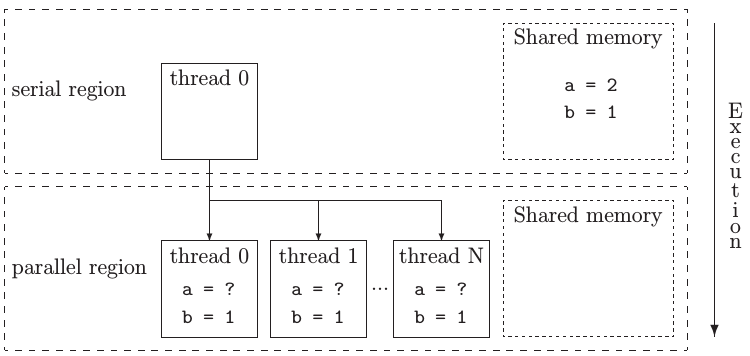
\includegraphics[width=0.80\textwidth]{figuras/reg-paralelaValPriv.png} \\
  \caption{Representaci\'on gr\'afica de las cl\'ausulas PRIVATE y FIRSTPRIVATE.} %
  \label{figRegparVarPriv}
\end{figure}

Al incluir la variable en una cl\'ausula FIRSTPRIVATE al inicio del alcance de una directiva toma autom\'aticamente el estatus de PRIVATE en dicho alcance y no es necesario incluirla en una cl\'ausula PRIVATE expl\'icitamente.
Al igual que con las variables PRIVATE debe tenerse en cuenta el costo de la operaci\'on desde el punto de vista computacional, al realizarse una copia de la variable y transferir la informaci\'on almacenada a la nueva variable.

\subsection{Otras Construcciones y Cl\'ausulas}
Existen m\'as construcciones de trabajo compartido, de sincronizaci\'on y de ambiente de datos, y m\'as cl\'ausulas en OpenMP, las cuales exceden el alcance de este trabajo de tesis y que pueden ser consultadas en el est\'andar OpenMP\citep{openmp} o en \citep{Her}.

\section{Proceso de optimizaci\'on}\label{sec:n6}
Dependiendo del prop\'osito de una aplicaci\'on, y de la forma como ser\'a utilizada, suelen considerarse tres principios de optimizaci\'on del desempe\~no\citep{Garg}
\begin{itemize}
\item Resolver el problema m\'as r\'apidamente
\item Resolver un problema m\'as grande en el mismo tiempo
\item Resolver el mismo problema en el mismo tiempo, pero utilizando una cantidad menor de recursos del sistema
\end{itemize}
En aplicaciones de HPC, obtener resultados m\'as r\'apidamente es crucial para los usuarios. Por ejemplo, para un ingeniero, representa una diferencia considerable poder repetir una simulaci\'on en el transcurso de una noche en lugar de esperar varios d\'ias para que la simulaci\'on termine. El tiempo ganado puede ser aprovechado para modificar el dise\~no, correr experimentos de mayor tama\~no, resolver problemas con conjuntos de datos m\'as grandes, u obtener resultados m\'as precisos. Por otro lado, cuando el tama\~no del problema y el tiempo de ejecuci\'on se mantengan constantes, una aplicaci\'on optimizada consumir\'a menos recursos para completar su ejecuci\'on\citep{Garg}.

El proceso de optimizaci\'on tiene algunas etapas fundamentales: ``desarrollo de la aplicaci\'on, optimizaci\'on serial, y optimizaci\'on paralela''.  La primera etapa abarca el dise\~no, programaci\'on y consideraciones de portabilidad de la aplicaci\'on, es decir, elecci\'on de algoritmos y estructuras de datos para resolver el problema. En el caso de este trabajo de tesis, esa etapa fue llevada a cabo por el autor de la aplicaci\'on en que basamos nuestro estudio. Las etapas de optimizaci\'on serial y optimizaci\'on paralela son las que ser\'an explicadas brevemente en esta subsecci\'on. En la Fig. \ref{figGySEtapas} (tomada de \citep{Garg}), podemos observar las etapas del proceso de optimizaci\'on.

Una decisi\'on importante para el proceso de optimizaci\'on es contemplar en qu\'e plataforma o conjunto de ellas se implementar\'a la aplicaci\'on. Esta decisi\'on incluye seleccionar sistema operativo y arquitectura de ejecuci\'on. La optimizaci\'on ser\'a m\'as focalizada mientras m\'as puntuales sean las decisiones tomadas, limitando el rango de plataformas en las cuales el programa puede ejecutarse\citep{Garg}. Una vez que el programa produzca resultados correctos, estar\'a listo para ser optimizado. Se seleccionar\'an un conjunto de casos de test para validar que el programa contin\'ue arrojando resultados correctos y se los utilizar\'a repetidamente en el transcurso de la optimizaci\'on.

\begin{figure}[htb]%[htp]
  \centering
  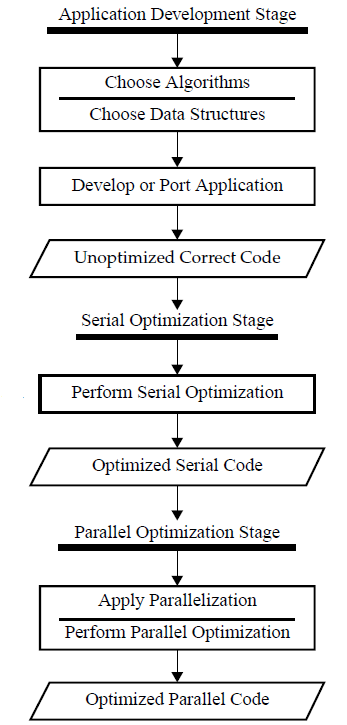
\includegraphics[width=0.40\textwidth]{figuras/g-and-s-etapas1.png} \\
  \caption{Etapas de Optimizaci\'on y Desarrollo de una Aplicaci\'on.} %
   \label{figGySEtapas}
\end{figure}

Tambi\'en se debe seleccionar un conjunto de casos para llevar a cabo pruebas de tiempo. Puede ser necesario que este conjunto sea diferente a los utilizados para validar el programa. Los casos de test para el cronometraje de tiempo podr\'ian ser varios ``benchmarks'' que representen adecuadamente el uso del programa. Se utilizar\'an estos benchmarks para medir el nivel de desempe\~no b\'asico o ``l\'inea de base'', de manera de disponer de datos fiables para utilizar m\'as tarde en las comparaciones de c\'odigo optimizado y c\'odigo original. De esta manera, se puede medir el efecto de la optimizaci\'on.

\subsection{Optimizaci\'on Serial}
La Optimizaci\'on Serial es un proceso iterativo que involucra medir repetidamente un programa seguido por la optimizaci\'on de sus partes cr\'iticas de rendimiento. La Fig. \ref{figGySSerial} (tomada de \citep{Garg}) resume las tareas de optimizaci\'on y da un diagrama de flujo simplificado para el proceso de optimizaci\'on serial.

\begin{figure}[h!]%[htp]
  \centering
  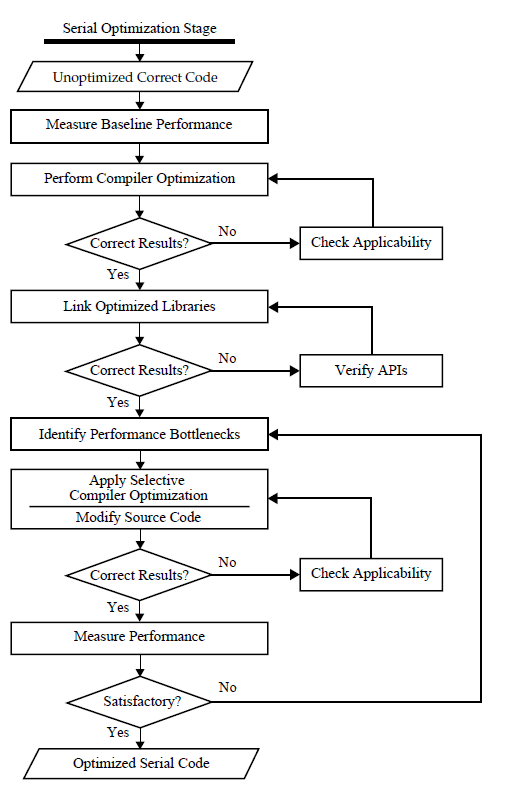
\includegraphics[width=0.60\textwidth]{figuras/g-and-s-serial1.png} \\
  \caption{Proceso de Optimizaci\'on Serial.} %
  \label{figGySSerial}
\end{figure}

Una vez que las mediciones de rendimiento de la l\'inea de base se han obtenido, el esfuerzo de optimizaci\'on debe iniciarse mediante la compilaci\'on de todo el programa con opciones seguras. Siguiente, linkear librer\'ias optimizadas. (Este linkeo es una manera sencilla de llevar implementaciones altamente optimizadas de operaciones estandar en un programa)
Luego de esto se debe verificar que los resultados preservan la correctitud del programa. Este paso incluye verificar que el programa realiza llamadas a las Interfaces de Programaci\'on de Aplicaci\'on (APIs sus siglas en Ingles) adecuadas en las librer\'ias optimizadas. Adem\'as, es recomendable que sea medido el desempe\~no del programa para verificar que ha mejorado.

El siguiente paso es identificar partes de desempe\~no cr\'iticas en el c\'odigo. El perfilado (profiling en Ingles) del c\'odigo fuente puede ser usado para determinar cuales partes del c\'odigo son las que toman m\'as tiempo para ejecutarse. Las partes identificadas son excelentes objetivos para enfocar el esfuerzo de optimizaci\'on, y las mejoras resultantes de desempe\~no pueden ser significativas. Otra t\'ecnica muy \'util para identificar estas partes de c\'odigo cr\'iticas es el monitoreo de la actividad del sistema y el uso de los recursos del sistema\citep{Garg}. 

\subsubsection{Metodolog\'ia de medici\'on}
Al trabajar en optimizar la performance de una aplicaci\'on, es esencial usar varias herramientas y t\'ecnicas que sugieran que partes del programa necesitan ser optimizadas, comparar el desempe\~no antes y luego de la optimizaci\'on y mostrar que tan eficiente los recursos del sistema han sido utilizados por el c\'odigo optimizado\citep{Garg}.

El primer paso en el proceso de afinaci\'on de la aplicaci\'on es cuantificar su desempe\~no. Este paso es alcanzado usualmente estableciendo un desempe\~no base y fijando expectativas apropiadas de cuanta mejora en el desempe\~no es razonable alcanzar.
Para programas cientificos, la m\'etricas de mayor inter\'es son usualmente el tiempo reloj (tiempo de respuesta) de un solo trabajo y aquellos que relacionan el desempe\~no de la aplicaci\'on a picos te\'oricos de desempe\~no de la CPU\citep{Garg}.
A traves de benchmarks es que podemos realizar an\'alisis de la performance de la aplicaci\'on. Una gu\'ia importante a seguir es que las mediciones deben ser reproducibles dentro de un rango de tolerancia esperado. Con esto en mente se definen las siguientes reglas generales:
\begin{itemize}
\item Seleccionar cuidadosamente los conjuntos de datos a utilizar. Deben representar adecuadamente el uso de la aplicaci\'on.
\item Al igual que en las mediciones en otros campos de la ingenier\'ia, la incertidumbre tambi\'en se aplica a las mediciones de desempe\~no de programas de computadora. El simple hecho de tratar de medir un programa se entromete en su ejecuci\'on y posiblemente lo afecta de manera incierta.
\item Siempre que sea posible, ejecutar los benchmarks desde un sistema de archivos tipo tmpfs (/tmp) o alg\'un sistema de archivos montado localmente. Ejecutar una aplicaci\'on desde un sistema de archivos montado por red introduce efectos de red irreproducibles en el tiempo de ejecuci\'on.
\item Actividades de paginado y swapeo deben ser monitoreadas mientras se ejecuta el benchmark, ya que estas pueden desvirtuar completamente la medici\'on.
\item Las mediciones de ``respuesta del programa'' deben ser desempe\~nadas en una manera dedicada, sin otros programas o aplicaciones ejecutandose.
\item Las caracteristicas del sistema deben ser registradas y guardadas.
\end{itemize}

\subsubsection{Herramientas de medici\'on}
Antes de analizar el desempe\~no de la aplicaci\'on, uno debe identificar los parametros que deben ser medidos y elegir herramientas acordes a las mediciones.
Las herramientas de medici\'on de desempe\~no pueden ser divididas en tres grupos\citep{Garg} basados en su funci\'on:
\begin{itemize}
\item Herramientas de temporizador, que miden el tiempo utilizado por un programa de usuario o sus partes. Pueden ser herramientas de l\'inea de comando o funciones dentro del programa.
\item Herramientas de perfilado, que utilizan resultados de tiempo para identificar las partes de mayor utilizaci\'on de una aplicaci\'on.
\item Herramientas de monitoreo, que miden la utilizaci\'on de varios recursos del sistema para identificar ``cuellos de botella'' que ocurren durante la ejecuci\'on.
\end{itemize}
Existen otras formas de categorizar estas herramientas, como puede ser basados en los requerimientos para su uso (herramientas que operan con binarios optimizados, o que requieren insertarse en el c\'odigo fuente, etc), o incluso dividirlas en dos grupos:
\begin{itemize}
\item Herramientas de medici\'on de desempe\~no serial
\item Herramientas de medici\'on de desempe\~no paralelo.
\end{itemize}

\subsubsection{Herramientas de medici\'on de tiempo}
El paso fundamental para evaluar comparativamente y poner a punto el desempe\~no de un programa es medir con precisi\'on la cantidad de tiempo utilizado ejecutando el c\'odigo. Generalmente uno est\'a interesado en el tiempo total utilizado para correr un programa, as\'i como en el tiempo utilizado en porciones del programa.
Para medir el programa completo es necesario usar herramientas que midan con precisi\'on el tiempo transcurrido desde el comienzo de la ejecuci\'on del programa. En GNU/Linux utilizamos la herramienta ``time'' para dicho prop\'osito. La forma de utilizar time es ejecutarlo desde una terminal de GNU/Linux pasando como par\'ametro el comando que debe medir tal cual como el comando es ejecutado normalmente. Por ejemplo:
\begin{lstlisting}[style=For, numbers=none]
	$ time  find / -name ``syslog''
\end{lstlisting}
El comando siendo medido realiza su ejecuci\'on normalmente. Al finalizar su ejecuci\'on, el comando time muestra por salida est\'andar tres valores (Fig. \ref{figTime}):
\begin{itemize}
\item ``real'': el tiempo real transcurrido entre el inicio y la finalizaci\'on de la ejecuci\'on.
\item ``user'': el tiempo de usuario del procesador.
\item ``sys'': el tiempo de sistema del procesador.
\end{itemize}

\begin{figure}[htbp]
  \begin{lstlisting}[style=consola, numbers=none]
  h4ndr3s@gondolin:~$ time find . -name "invisidos*"
  ./t3sis/tesis/source/invisidos2fin.for
  ./t3sis/tesis/source/invisidos2fin_OMP_def.for
  ./t3sis/tesis/source/invisidos2fin_OMP-origfuncionando.for
  ./t3sis/tesis/source/invisidos2fin_OMP_80.for

  real    0m0.089s
  user    0m0.060s
  sys     0m0.024s
  \end{lstlisting}
  \caption{Ejemplo de ejecuci\'on del comando \emph{time}.} %
  \label{figTime}
\end{figure}

\subsubsection{Herramientas de perfilado de programa}
El perfilado muestra cuales funciones son las m\'as costosas en las ejecuciones de una aplicaci\'on. Es necesario utilizar para la medici\'on casos de test representativos y multiples, de manera de obtener resultados significativos.
En GNU/Linux se cuenta con la herramienta ``gprof'' para realizar perfilado de aplicaciones. Para utilizarla un programa debe estar compilada con la opci\'on ``-pg''. Luego se ejecuta el programa una vez y genera un archivo llamado gmon.out en el directorio de ejecuci\'on el cual es utilizado por el comando gprof para generar el reporte de perfilado para esa ejecuci\'on. La sintaxis de gprof es:
\begin{lstlisting}[style=For, numbers=none]
	$ gprof  <programa_ejecutable>  [<ruta_a_gmon.out>]
\end{lstlisting}
Si no se le pasa la ruta a gmon.out, por defecto utiliza el directorio desde donde es invocado gprof. Un ejemplo de este proceso puede verse a continuaci\'on: 

\begin{lstlisting}[style=For, numbers=none]
    $ gfortran -pg foo.for -o foo
    $ foo
    $ gprof foo
\end{lstlisting}
La salida de gprof es por salida est\'andar y bastante extensa, por lo cual es aconsejable redirigirla a un archivo. Consta de tres partes: la primera parte lista las funciones ordenadas de acuerdo al tiempo que consumen, junto con sus descendientes (tiempo inclusivo). La segunda parte lista el tiempo exclusivo para las funciones (tiempo empleado ejecutando la funci\'on) junto con los porcentajes de tiempo total de ejecuci\'on y n\'umero de llamadas. La \'ultima parte da un \'indice de todas las llamadas realizadas en la ejecuci\'on.

\subsection{Optimizaci\'on Paralela}
Luego de que la aplicaci\'on est\'a optimizada para procesamiento secuencial, su tiempo de ejecuci\'on puede ser  reducido a\'un m\'as permitiendo que se ejecute en varios procesadores. Las t\'ecnicas m\'as usadas comunmente para paralelizaci\'on son el uso expl\'icito de hilos, el uso de directivas al compilador y el pasaje de mensajes\citep{Garg}. En la Fig. \ref{figGySParalel} (tomada de \citep{Garg}) se ve ilustrado el proceso de optimizaci\'on paralela.

\begin{figure}[h!]%[htp]
  \centering
  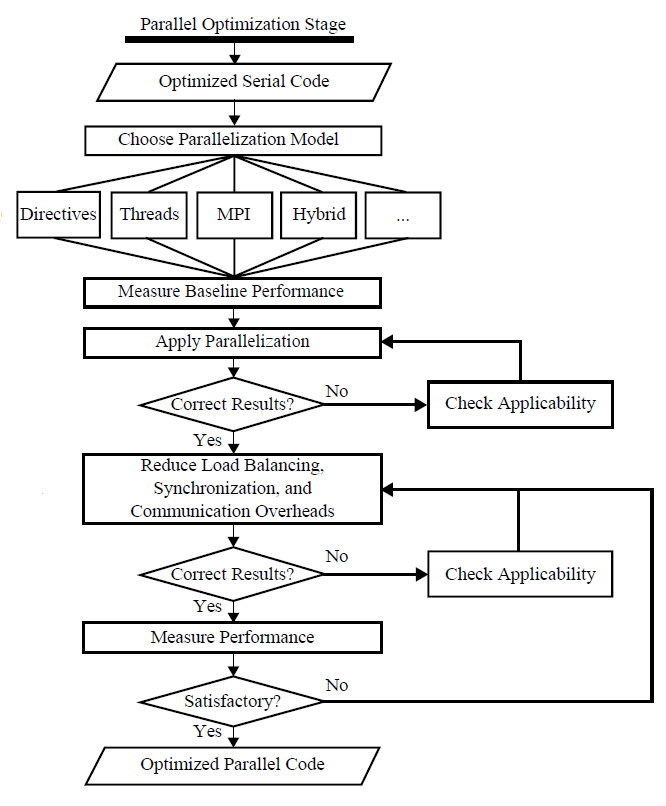
\includegraphics[width=0.65\textwidth]{figuras/g-and-s-paralel1.png} \\
  \caption{Proceso de Optimizaci\'on Paralela.} %
  \label{figGySParalel}
\end{figure}

El primer paso es elegir un modelo, identificar que partes del programa deben ser paralelizadas y determinar como dividir la carga de trabajo computacional entre los diferentes procesadores. Dividir la carga de trabajo computacional es crucial para el desempe\~no, ya que determina los gastos generales de comunicaci\'on, sincronizaci\'on y de desequilibrios de carga resultantes en un programa paralelizado. Generalmente, una divisi\'on de trabajo de ``nivel grueso'' es recomendada debido a que minimiza la comunicaci\'on entre las tareas paralelas, pero en algunos casos, un enfoque de este tipo lleva a balanceo de carga muy pobre; un nivel m\'as fino en el particionamiento de la carga de trabajo puede llevar a un mejor balanceo de carga y desempe\~no de la aplicaci\'on.

Luego de seleccionado un modelo de paralelizaci\'on e implementado, lo siguiente es optimizar su desempe\~no. Similar a la optimizaci\'on serial, este proceso es iterativo e involucra mediciones repetidas seguidas de aplicar una o m\'as t\'ecnicas de optimizaci\'on para mejorar el desempe\~no del programa. Las aplicaciones paralelas, sin importar el modelo utilizado, necesitan que exista comunicaci\'on entre los procesos o hilos concurrentes. Se debe tener cuidado de minimizar los gastos extras en comunicaci\'on y asegurar una sincronizaci\'on eficiente en la implementaci\'on; Minimizar el desequilibrio de cargas entre las tareas paralelas, ya que esto degrada la escalabilidad del programa. Tambi\'en se debe considerar temas como migraci\'on y programaci\'on de procesos, y coherencia de cache. Las librer\'ias del compilador pueden ser utilizadas para implementar versiones paralelas de funciones usadas comunmente, tanto en aplicaciones multihilo como multiproceso.

Los cuellos de botella de un programa paralelo pueden ser muy diferentes de los presentes en una versi\'on secuencial del mismo programa. Adem\'as de gastos extras espec\'ificos de la paralelizaci\'on, las porciones lineales (o secuenciales) de un programa paralelo pueden limitar severamente la ganancia de velocidad de la paralelizaci\'on. En tales situaciones , hay que prestar atenci\'on a esas porciones secuenciales para mejorar el desempe\~no total de la aplicaci\'on paralela. Por ejemplo, consideremos la soluci\'on directa de N ecuaciones lineales. El costo computacional escala en el orden de $O(N^3)$ en la etapa de descomposici\'on de la matriz y en el orden de $O(N^2)$ en la etapa de sustituci\'on adelante-atr\'as. En consecuencia, la etapa de sustituci\'on adelante-atr\'as apenas se nota en el programa secuencial, y el desarrollador paralelizando el programa justificadamente se enfoca en la etapa de descomposici\'on de la matriz. Posiblemente, como resultado del trabajo de paralelizaci\'on, la etapa de descomposici\'on de la matriz se vuelve m\'as eficiente que la etapa de sustituci\'on adelante-atr\'as. El desempe\~no total y velocidad del programa de resoluci\'on directa ahora est\'a limitado por el desempe\~no de la etapa de sustituci\'on adelante-atr\'as. Para mejorar a\'un m\'as el desempe\~no, la etapa de sustituci\'on adelante-atr\'as deber\'ia convertirse en el foco de optimizaci\'on y posiblemente un trabajo de paralelizaci\'on\citep{Garg}.

\section{Caso de Estudio: Modelizaci\'on del Flujo Inv\'iscido}\label{sec:n7}
El programa objeto de optimizaci\'on de esta tesis es de autor\'ia de Ricardo A. Prado, docente e investigador de la Universidad Nacional del Comahue, y fue utilizado para obtener resultados para su trabajo de tesis de doctorado\citep[Mayo 2007]{Prado} en el \'area de Ingenier\'ia presentado en la Universidad de Buenos Aires en 2007. Como se expone en dicho trabajo, la tesis ``analiza el comportamiento fluidodin\'amico de una turbom\'aquina particular: la turbina e\'olica''. La creaci\'on del programa se justifica en el mismo trabajo porque ``debido a la complejidad de las ecuaciones de gobierno en ambas zonas del campo fluidodin\'amico, como as\'i tambi\'en de la geometr\'ia de la turbina y de sus condiciones de operaci\'on, se requiere de procesos de resoluci\'on num\'erica adecuados, los cuales se incorporaron en los c\'odigos computacionales que se desarrollaron a tal efecto''.

El modelo matem\'atico que implementa el programa es la ``Ley de Biot-Savart''\footnote{\url{https://es.wikipedia.org/wiki/Ley_de_Biot-Savart}}, que indica el campo magn\'etico creado por corrientes el\'ectricas estacionarias. Es una de las leyes fundamentales de la magnetoest\'atica. En particular, en el trabajo de Prado se aplica a una modelizaci\'on del flujo inv\'iscido (de viscosidad despreciable, casi nula) alrededor de la pala de la turbina. El modelo num\'erico se formula a trav\'es del m\'etodo de los paneles. El objetivo de la aplicaci\'on de la Ley de Biot-Savart en el trabajo es el c\'alculo de las velocidades de flujo inducidas en un punto para cada panel de la pala. 

El programa realiza el c\'alculo de una integraci\'on por el m\'etodo de Simpson. La regla o m\'etodo de Simpson es un m\'etodo de integraci\'on num\'erica que se utiliza para obtener la aproximaci\'on de una integral en un intervalo definido, al dividir ese intervalo en subintervalos y aproximar cada subintervalo con un polinomio de segundo grado. 
\label{pagcap3}
\chapter{Optimizaci�n e implementaci\'on de multiprocesamiento}

\section{Introducci\'on}
En los cap\'itulos anteriores presentamos la problem\'atica por la cual surge la idea y la necesidad de paralelizar la programaci\'on, as\'i como las herramientas a utilizar, en nuestro caso OpenMP bajo Fortran. La elecci\'on del lenguaje Fortran se debe a que el usuario de la aplicaci\'on utilizada es tambi\'en su creador, de manera que, para hacer el cambio lo m\'as transparente posible, se decide no alterar este aspecto del programa.

Con Fortran como base, y teniendo en cuenta la estructura del programa con un an\'alisis inicial del mismo, debido a las caracter\'isticas de programa estructurado, monol\'itico y no modularizado, se elige orientar la soluci\'on a aplicar concurrencia en un entorno de Memoria Compartida y dejar habilitada la ejecuci\'on paralela en un equipo multiprocesador.

La aplicaci\'on bajo estudio utiliza archivos de datos en disco para guardar resultados, tanto parciales como finales. Esta actividad de entrada/salida introduce importantes demoras en el tiempo de respuesta, que necesitamos considerar. En este cap\'itulo describiremos el proceso seguido para la optimizaci\'on del c\'odigo Fortran en lo relacionado con el manejo de los archivos. Esta primera fase de optimizaci\'on permitir\'a la paralelizaci\'on de segmentos de c\'odigo.

Tambi\'en realizaremos un an\'alisis del perfil de ejecuci\'on de la aplicaci\'on con una herramienta de perfilado  que permitir\'a identificar qu\'e subrutinas son las que m\'as tiempo consumen y cu\'ales son las m\'as indicadas para aplicar la paralelizaci\'on.

Por \'ultimo veremos la forma como se ha aplicado OpenMP a las partes seleccionadas de la aplicaci\'on. Explicaremos por qu\'e han sido seleccionadas ciertas construcciones espec\'ificas del c\'odigo y las razones de modificar algunas estructuras de control para hacer m\'as eficiente la utilizaci\'on de la memoria y de la CPU.


\section{An\'alisis de la aplicaci\'on}
Primero se analiz\'o la aplicaci\'on para poder proceder con su optimizaci\'on y paralelizaci\'on. Como se explic\'o  en la secci\'on \ref{sec:n6}, determinamos la plataforma en que deber\'ia ejecutarse la aplicaci\'on, estableciendo versi\'on de sistema operativo  y arquitectura. La aplicaci\'on recibida fue utilizada por su programador, en arquitectura x86 de 32 bits, bajo sistema operativo GNU/Linux, espec\'ificamente con la distribuci\'on CentOS. 

Lo primero fue obtener resultados base de ejecuciones de la aplicaci\'on bajo ese entorno, a fin de tener una referencia para la comparaci\'on de resultados. El autor de la aplicaci\'on nos indic\'o que la misma es completamente determin\'istica, con lo cual la aplicaci\'on, con los mismos datos de entrada provistos, debe arrojar los mismos resultados en todas las ejecuciones. 

Para llevar a cabo el trabajo de la Tesis se seleccion\'o el entorno GNU/Linux, con la distribuci\'on Slackware de 64 bits como base, a la cual no fue necesario agregar componentes ni efectuar ninguna compilaci\'on especial. Se verific\'o que la aplicaci\'on entregada por el usuario compilara correctamente sin ninguna modificaci\'on en esta plataforma y arrojara, para los datos de entrada, exactamente los mismos resultados que en su entorno original. 

Con esto ya verificado se avanz\'o en el trabajo de Tesis hacia el an\'alisis propiamente dicho de la aplicaci\'on. 

Como vimos en el cap\'itulo anterior, lo primero antes de optimizar es tener una aplicaci\'on que produzca resultados correctos. En nuestro caso se nos present\'o una aplicaci\'on ya depurada y funcionando correctamente, por lo cual no debimos preocuparnos por esta parte, as\'i que pasamos a la parte de optimizaci\'on, donde se deben seleccionar previamente los casos de test para validar que la optimizaci\'on sigue produciendo resultados correctos.

Contamos con dos casos de test provistos por el creador de la aplicaci\'on, los cuales se identifican por dos par\'ametros (nr y no) que definen, respectivamente, la cantidad total de palas y de nodos sobre los cuales se va a realizar la simulaci\'on. Con estos par\'ametros se definen los casos de test, con valores iguales para ambos datos: nr = no = 50 en el primer caso de test, y nr = no = 80 en el segundo caso.

Estos valores tambi\'en definen unas variables globales comunes de la aplicaci\'on llamadas ``maxir'' y ``maxio'' que se fijan a nr+1 y no+1 respectivamente. Los valores est\'an codificados directamente en la aplicaci\'on y no se utiliza ning\'un tipo de constante simb\'olica que los defina, algo que ser\'ia m\'as adecuado para el tratamiento de dichos valores y para tener un c\'odigo m\'as limpio; esto no se modific\'o y se mantuvo el tratamiento original de los valores para alterar lo menos posible el c\'odigo. 

Por el mismo motivo, tampoco se modific\'o la obtenci\'on de los valores de entrada para las simulaciones a partir de un archivo de texto.

\subsection{An\'alisis de perfilado}\label{ssec:perfilado}
Como paso preliminar de la optimizaci\'on realizamos an\'alisis de la aplicaci\'on con la herramienta de perfilado gprof, para poder comparar los principales puntos de consumo de tiempo con anterioridad a la optimizaci\'on y luego de la misma. De esta forma se pretende seleccionar una o varias subrutinas para la paralelizaci\'on y observar de qu\'e manera cambia el comportamiento de la aplicaci\'on con la optimizaci\'on.

Los datos obtenidos mediante gprof en esta etapa muestran que la subrutina ``estela'' resulta ser la que consume el mayor porcentaje, 79,83\% del tiempo de ejecuci\'on de la aplicaci\'on. Le sigue la subrutina ``solgauss'' con un 14,36\%. Estos datos se pueden observar en la Fig. \ref{figGprof1}.

\begin{figure}[h!]%[htp]
  \centering
  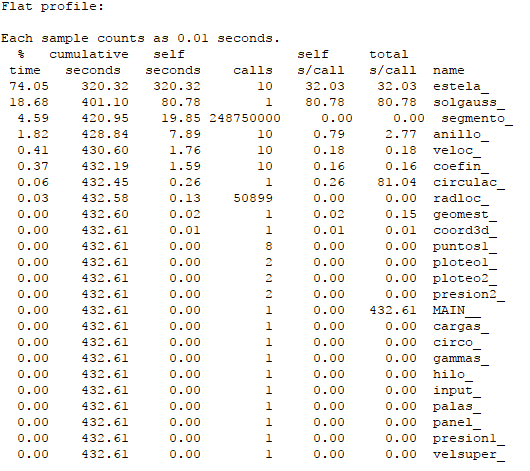
\includegraphics[width=0.60\textwidth]{figuras/gprof1.png} \\
  \caption{Salida de \emph{gprof} en el primer equipo.} %
   \label{figGprof1}
\end{figure}

Con estos resultados se pudo inferir en esta primer revisi\'on que estas dos subrutinas son las candidatas a ser optimizadas con procesamiento paralelo.

Para las pruebas se utilizaron dos computadoras de escritorio distintas, ambas multiprocesadores. El primer equipo posee un procesador AMD Phenom II con 4 nucleos y 4GB de memoria RAM. El segundo equipo consta de un procesador Intel Core i3 con 2 n\'ucleos (2 hilos cada procesador) y 6 Gb de RAM. Las especificaciones completas son provistas en el Cap\'itulo 4 donde se analizan los resultados obtenidos.

La salida de la Fig. \ref{figGprof1} fue obtenida en el primer equipo. Realizamos el mismo an\'alisis de perfilado sobre el segundo equipo, y observamos que la mayor porci\'on del tiempo sigue siendo consumida por la subrutina ``estela'' seguida por ``solgauss'' casi en los mismos porcentajes, 74,26\% y 16,84\% respectivamente. Tambi\'en es de notar la mejora en los tiempos de ejecuci\'on. Esto se puede observar en la Fig. \ref{figGprof2}.

\begin{figure}[h!]%[htp]
  \centering
  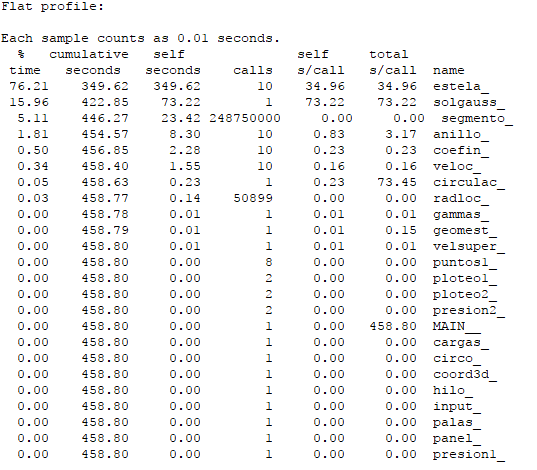
\includegraphics[width=0.60\textwidth]{figuras/gprof2.png} \\
  \caption{Salida de \emph{gprof} en el segundo equipo.} %
   \label{figGprof2}
\end{figure}

A esta altura del trabajo contamos con ``c\'odigo correcto no optimizado'' (Unoptimized Correct Code)\citep{Garg}, de modo que, siguiendo las etapas del proceso de optimizaci\'on (ilustradas en \ref{figGySEtapas}) visto en el cap\'itulo 2, debemos efectuar una optimizaci\'on serial para obtener c\'odigo optimizado. Luego de esto podremos pasar a la etapa de ``Optimizaci\'on Paralela'', donde aplicaremos paralelizaci\'on al c\'odigo para obtener justamente c\'odigo paralelo optimizado. 

En las siguientes secciones veremos c\'omo realizamos estas dos etapas del proceso para obtener nuestra aplicaci\'on de estudio en forma optimizada paralela.

\section{Optimizaci\'on Serial del c\'odigo Fortran}
La optimizaci\'on serial es ``un proceso iterativo que involucra medir repetidamente un programa seguido de optimizar sus porciones cr\'iticas''\citep{Garg}. Obtenidas las mediciones iniciales del comportamiento, debemos optimizar las opciones de compilaci\'on y vincular  el c\'odigo objeto con bibliotecas optimizadas. En el trabajo de tesis intentamos reducir al m\'inimo las modificaciones al c\'odigo, por lo cual las opciones que se utilizar\'an para la compilaci\'on ser\'an \'unicamente las referidas a la infraestructura de programaci\'on paralela de OpenMP. 

Por lo dem\'as, la aplicaci\'on no hace uso de ninguna otra biblioteca que no se cuente entre las que utiliza regularmente el compilador para construir la aplicaci\'on. Como buscamos observar el impacto de optimizar serialmente el c\'odigo y aplicar paralelizaci\'on, no se utilizan bibliotecas que pudieran optimizar otras partes del programa.

\subsection{An\'alisis del acceso a datos de la aplicaci\'on}
Al analizar los resultados de ejecuci\'on de la aplicaci\'on observamos que maneja gran cantidad de archivos en disco, tanto de texto como binarios (temporales). En el directorio de la aplicaci\'on aparecen 34 archivos de extensi\'on TXT, 9 archivos PLT, 5 archivos OUT y 8 archivos TMP. A \'estos se agregan el propio archivo fuente .for, el ejecutable invisidosExe, el archivo con los datos de entrada entvis2f.in, y el que utilizamos para almacenar los datos de gprof, invisidosExegprof. En la Fig. \ref{consLS} se puede observar el listado del directorio de ejecuci\'on.\\
\begin{figure}[h!]%[htp]
  \begin{lstlisting}[style=consola, numbers=none]
        h4ndr3s@gondolin:~/pruebas/oldone\$ ls
        alfa.txt    	cp2.txt      	integ1.txt         	vel02int.txt
        arco.txt    	cpei.plt     	integ2.txt         	vel02pvn.txt
        cindg.tmp   	cpei.txt     	invisidos2fin.for  	   velcapae.txt
        circo.txt   	cr.txt       	invisidosExe*           velcapai.txt
        cix1.tmp    	entvis2f.in  	invisidosExegprof       velindad.plt
        cix2.tmp    	estel1.txt   	palas.plt          	velindad.txt
        ciy1.tmp    	estel2.txt   	palest.plt         	velpotad.txt
        ciy2.tmp    	estel3.txt   	panel.plt          	velresad.plt
        ciz1.tmp    	fuerza.plt   	panel.txt          	veltotal.txt
        ciz2.tmp    	fzas.txt     	pres.plt           	velxyz.txt
        co.txt      	gama.txt     	salida2.out        	vix.txt
        coefg.tmp   	gdifo.out    	subr.out           	viy.txt
        coefp.txt   	gdifr.out    	vector.plt         	viz.txt
        coord.txt   	gmon.out     	vel01ext.txt       	vn.txt
        cp075c.txt  	go.out       	vel01int.txt
        cp1.txt     	gr.out       	vel02ext.txt
  \end{lstlisting}
  \caption{Listado del directorio luego de la ejecuci\'on del programa}
  \label{consLS}
\end{figure}
Los tama\~nos de la mayor\'ia de los archivos van desde 8 KB hasta 2 MB, pero los archivos TMP pueden alcanzar un tama\~no de varios megabytes (se observan algunos del orden de los cientos de megabytes). Esto evidencia que una corrida de la aplicaci\'on intercambia un volumen significativo de datos entre la aplicaci\'on y el sistema de archivos.

Con el fin de localizar los puntos de aplicaci\'on de la optimizaci\'on, relevamos la relaci\'on entre cada archivo y las subrutinas que lo acceden, indicando las operaciones realizadas (escritura, lectura, lectura/escritura, rewind). De este relevamiento se obtiene la lista de archivos que \'unicamente son escritos en disco, y los que son adem\'as le\'idos, por cada subrutina. La relaci\'on de archivos y subrutinas se muestra en la tabla \ref{tab:tabArch}.\\

\begin{table}[htb]
\begin{center}
\begin{tabular}{|c|c|c|}
\hline 
\rule[-1ex]{0pt}{2.5ex} Archivos & Funci\'on & Operaci\'on \\ 
\hline 
\hline
\rule[-1ex]{0pt}{2.5ex} cpei.plt, cpei.txt & presion2 & write only \\ 
\hline 
\rule[-1ex]{0pt}{2.5ex} palest.plt & palas, geomest & write only \\ 
\hline 
\rule[-1ex]{0pt}{2.5ex} palas.plt, alfa.txt, coord.txt & palas & write only \\ 
\hline 
\rule[-1ex]{0pt}{2.5ex} panel.plt, panel.txt & panel & write only \\ 
\hline 
\rule[-1ex]{0pt}{2.5ex} pres.plt, cp075c.txt, coefp.txt, & presion1 & write only \\ 
%\hline 
\rule[-1ex]{0pt}{2.5ex}  cp1.txt, cp2.txt &  &  \\ 
\hline 
\rule[-1ex]{0pt}{2.5ex} velxyz.txt, velpotad.txt, velindad.txt &  & \\ 
%\hline 
\rule[-1ex]{0pt}{2.5ex} velcapae.txt, velcapai.txt, vix.txt & veloc & write only \\ 
%\hline 
\rule[-1ex]{0pt}{2.5ex} viy.txt, viz.txt &  &  \\ 
\hline 
\rule[-1ex]{0pt}{2.5ex} estel1.txt, estel2.txt, estel3.txt & geomest & write only \\ 
\hline 
\rule[-1ex]{0pt}{2.5ex} \multirow{2}{1cm}{gama.txt} & circulac & write only \\ \cline{2-3}
& gammas & read only \\ \cline{1-3} 
\hline 
\rule[-1ex]{0pt}{2.5ex} veltotal.txt, vel01ext.txt, vel01int.txt & velsuper & write only \\ 
%\hline 
\rule[-1ex]{0pt}{2.5ex} vel02ext.txt, vel02int.txt, vel02pvn.txt &  &  \\ 
\hline 
\rule[-1ex]{0pt}{2.5ex} velresad.plt & ploteo2 & write only \\ 
\hline 
\rule[-1ex]{0pt}{2.5ex} \multirow{2}{1cm}{arco.txt} & circulac & write only \\ \cline{2-3} 
& circo & read only \\ \cline{2-3}
\hline 
\rule[-1ex]{0pt}{2.5ex} fzas.txt, fuerza.plt, vector.plt & cargas & write only \\ 
\hline 
\rule[-1ex]{0pt}{2.5ex} \multirow{2}{1cm}{coefg.tmp, cindg.tmp} & circulac & write y rewind \\ \cline{2-3}
& solgauss & read y rewind \\ \cline{2-3}
\hline 
\rule[-1ex]{0pt}{2.5ex} \multirow{2}{1cm}{cix1.tmp, ciy1.tmp, ciz1.tmp} & anillo & write y rewind \\ \cline{2-3}
& coefin & read y rewind \\ \cline{2-3}
& - & - \\ \cline{2-3}
\hline 
\rule[-1ex]{0pt}{2.5ex} \multirow{3}{1cm}{cix2.tmp, ciy2.tmp, ciz2.tmp} & coefin & write y rewind \\ \cline{2-3} 
& circulac & read y rewind \\ \cline{2-3}
& veloc & read y rewind \\ \cline{2-3}
\hline 
\rule[-1ex]{0pt}{2.5ex} \multirow{4}{1cm}{salida2.out} & input & write only \\ \cline{2-3}
& cargas & write only \\ \cline{2-3}
& anillo & write only \\ \cline{2-3}
& veloc & write only \\ \cline{2-3}
%\hline 
\hline 
\end{tabular} 
\caption {Relaci\'on archivos y funciones de la aplicaci\'on}
\label{tab:tabArch}
\end{center}
\end{table}

Fortran ofrece los archivos regulares, o archivos externos soportados en disco (External Files), pero tambi\'en los archivos internos o Internal Files, que son cadenas de caracteres o arreglos de cadenas de caracteres, localizados en memoria principal. Los Internal Files se manejan con las mismas funciones que los archivos externos, y la \'unica restricci\'on para su uso es la cantidad de memoria virtual del sistema. 
Como la latencia de los accesos a disco magn\'etico es, normalmente, al menos cinco \'ordenes de magnitud mayor que la de los accesos a memoria principal\citep{Gregg}, cambiando la definici\'on de los archivos en disco a Internal Files (siempre que la restricci\'on de tama\~no del sistema de memoria virtual lo permita) conseguimos una mejora sustancial de performance de la aplicaci\'on, sin ninguna modificaci\'on importante al c\'odigo ni al comportamiento del programa.

\subsection{Optimizaci\'on por adaptaci\'on de archivos externos a internos}
La primera decisi\'on tomada para la optimizaci\'on del c\'odigo es reducir el impacto de los accesos a archivos en disco que son le\'idos y adem\'as escritos por la aplicaci\'on. No efectuaremos ninguna modificaci\'on sobre los archivos que son \'unicamente escritos por las subrutinas, con cuatro excepciones: la escritura de los archivos integ1.txt e integ2.txt en la subrutina estela, retrasada hasta el final de la misma, y los archivos salida2.out, que guarda resultados de la ejecuci\'on a medida que avanza, y subr.out, que recoge lo mostrado en salida est\'andar. 
Estos archivos se guardar\'an en objetos de tipo Internal File de Fortran y su escritura se demorar\'a hasta la finalizaci\'on del programa. La elecci\'on de no pasar m�s archivos a Internal Files es para evitar un incremento elevado en la cantidad de memoria utilizada por la aplicaci\'on.
%OSO POR QUE? %HANDRU por lo indicado m�s adelante, ocupar m�s memoria con m�s archivos
Un caso especial es el Internal File \emph{outstd} que lleva lo impreso en salida est\'andar dentro de algunas subrutinas(estela, geomest, etc), y es mostrado por pantalla al retornar dichas subrutinas al programa principal.

Luego, todo archivo o External File que sea escrito y le\'ido durante la ejecuci\'on de la aplicaci\'on ser\'a mantenido por un Internal File. La \'unica modificaci\'on necesaria al c\'odigo ser\'a el cambio de las referencias a los archivos en las sentencias ``write'', ``read'' y ``rewind''. En la Fig. \ref{codSinMod} se muestra un ejemplo de c\'odigo previo a la modificaci\'on, y en la Fig. \ref{codModif} el c\'odigo ya modificado.\\

\begin{figure}[htb]%[htp]
%  \begin{lstlisting}[style=For, numbers=none]
   \begin{BVerbatim}
      open(unit=15,file='subr.out')
      ...
      write(15,1)
      write(6,1)
   \end{BVerbatim}
%  \end{lstlisting}
  \caption{Ejemplo de c\'odigo sin modificar}
  \label{codSinMod}
\end{figure}


Como se ve, reemplazamos el archivo ``subr.out'' representado por el identificador de unidad 15 por el Internal File denominado subrout.

\begin{figure}[htb]%[htp]
%  \begin{lstlisting}[style=For, numbers=none]
   \begin{BVerbatim}
      character subrout(500)*60   ! Internal File
      ...
      write(subrout(nsubr),1)
      nsubr=nsubr+1
    !      write(15,1)
      write(6,1)
   \end{BVerbatim}
%  \end{lstlisting}
  \caption{Ejemplo de c\'odigo modificado para utilizar Internal File}
  \label{codModif}
\end{figure}

Como se ha dicho, el External File subr.out pasa a ser manejado como un Internal File, que como se ve en la declaraci\'on de la Fig. \ref{codModif}, es un arreglo de 500 cadenas de 60 caracteres como m\'aximo. La variable nsubr mantiene la posici\'on en el internal file a ser escrita, y el argumento ``1'' en los comandos write es un formato de escritura definido dentro del programa como se explicaba en el cap\'itulo anterior.
En la tabla \ref{tab:tabEquiv} vemos c\'omo quedan las equivalencias de los External Files y su correspondiente cambio a Internal File.

\begin{table}[htb]
\begin{center}
\begin{tabular}{|c|c|}
\hline 
\rule[-1ex]{0pt}{2.5ex} Archivo en Disco & Internal File \\ 
\hline 
\hline
\rule[-1ex]{0pt}{2.5ex} integ1.txt & integ1 \\
\hline
\rule[-1ex]{0pt}{2.5ex} integ2.txt & integ2 \\
\hline
\rule[-1ex]{0pt}{2.5ex} salida2.out & salida2out \\
\hline
\rule[-1ex]{0pt}{2.5ex} subr.out & subrout \\
\hline
\rule[-1ex]{0pt}{2.5ex} gama.txt & gamastr \\
\hline
\rule[-1ex]{0pt}{2.5ex} circo.txt & circostr \\
\hline
\rule[-1ex]{0pt}{2.5ex} coefg.tmp & coefgtmp \\
\hline
\rule[-1ex]{0pt}{2.5ex} cindg.tmp & cindgtmp \\
\hline
\rule[-1ex]{0pt}{2.5ex} cix1.tmp & cix1tmp \\
\hline
\rule[-1ex]{0pt}{2.5ex} ciy1.tmp & ciy1tmp \\
\hline
\rule[-1ex]{0pt}{2.5ex} ciz1.tmp & ciz1tmp \\
\hline
\rule[-1ex]{0pt}{2.5ex} cix2.tmp & cix2tmp \\
\hline
\rule[-1ex]{0pt}{2.5ex} ciy2.tmp & ciy2tmp \\
\hline
\rule[-1ex]{0pt}{2.5ex} ciz2.tmp & ciz2tmp \\
\hline
\rule[-1ex]{0pt}{2.5ex} <salida est\'andar> & outstd \\
\hline 
\end{tabular} 
\caption {Equivalencias Archivo en Disco (External File) a Internal File.}
\label{tab:tabEquiv}
\end{center}
\end{table}

El proceso fue realizado primero en la subrutina Estela, buscando mejorar sus tiempos al convertir el manejo de los archivos integ1.txt e integ2.txt en internal files, retrasando la escritura en disco de los datos hasta el final de la subrutina. Lo primero que se observa luego de esta modificaci\'on es un comprensible incremento del uso de memoria de la aplicaci\'on, pasando de un uso de 200 a 202 MB, originalmente, sin aplicar ninguna modificaci\'on, a utilizar 205 MB con la modificaci\'on indicada en el tratamiento de los archivos. Es un cambio en principio poco significativo, pero con las modificaciones sucesivas se ver\'a el impacto en la utilizaci\'on de memoria.

De acuerdo a la tabla de funciones y archivos, y al an\'alisis efectuado mediante gprof, procedimos a modificar las subrutinas Solgauss y Circulac que son las que leen y escriben los archivos TMP respectivamente, archivos que consumen la mayor cantidad de espacio en disco de los utilizados por la aplicaci\'on.
Antes de realizar el cambio directamente, analizamos qu\'e estructura ser\'ia la m\'as adecuada para alojar los resultados, ya que los archivos TMP eran binarios sin formato, que transportaban valores calculados de una subrutina a otra.

Seleccionamos primero los archivos coefg.tmp y cindg.tmp (definidos como units 40 y 41 respectivamente al principio de la aplicaci\'on original) ya que eran los de menor tama\~no de todos los archivos tipo TMP. Como observamos en la tabla \ref{tab:tabArch}, los archivos mencionados son escritos en la subrutina ``circulac'' y leidos en ``solgauss'' (adem\'as de los rewind).

La subrutina circulac, como indica en sus comentarios realiza el ``c\'alculo de la circulaci\'on asociada a la estela y a cada anillo vorticoso''. Est\'a dividida en tres partes, siendo la primer parte la que realiza la escritura de los archivos coefg.tmp y cindg.tmp, y donde para estos c\'alculos lee los archivos tmp cix2.tmp, ciy2.tmp y ciz2.tmp, los cuales no son modificados en esta etapa. La segunda parte realiza la resoluci\'on de un sistema de npa*npa ecuaciones algebraicas y lo hace llamando a la subrutina solgauss que veremos a continuaci\'on. En la tercer parte con los resultados obtenidos se calculan otros valores que se escriben en otros archivos de resultados.

Como la subrutina ``circulac'' es la que crea los archivos coefg.tmp y cindg.tmp analizamos las estructuras de control utilizadas para generar dichos archivos. 

El bucle externo controlado por el ``do 1'' realiza el equivalente a npan iteraciones, con lo cual podemos concluir que el archivo determinado por la unit 41 (lo sabemos por el write(41)), es decir cindg.tmp, almacena un total de npan resultados. El bucle interno controlado por el ``do 2'' realiza npan * npan iteraciones, por lo tanto el archivo determinado por la unit 40 (write(40)), i.e. coefg.tmp, almacena npan * npan resultados. 

Analizado esto podemos definir que los tama\~nos de nuestros Internal Files para dichos archivos ser\'an de npan y npan * npan. Luego podemos ver que las variables coefg y cindg que almacenan los resultados para escribir en los archivos no est\'an tipificadas explicitamente en el c\'odigo, con lo cual observamos en el bloque common de toda la aplicaci\'on (repetido en cada subrutina) que se realiza la siguiente declaraci\'on:
\begin{lstlisting}[style=For, numbers=none]
  implicit real*8 (a-h,o-z)
\end{lstlisting}
la que indica que cualquier variable no tipificada definida en el c\'odigo cuyo nombre comience con una letra entre los rangos indicados (a-h y o-z) ser\'a declarada, impl\'icitamente, como real * 8, por lo cual podemos asegurar que coefg y cindg son de tipo real * 8. Con esto determinado podemos declarar Internal Files de tipo real * 8 de tama\~nos npan y npan * npan para reemplazar a cindg.tmp y coefg.tmp respectivamente:
\begin{lstlisting}[style=For, numbers=none]
  real*8 cindgtmp(npan),coefgtmp(npan*npan)
\end{lstlisting}
siendo cindgtmp el Internal File para cindg.tmp y coefgtmp el Internal File para coefg.tmp.

Ahora debemos reemplazar las escrituras de los archivos binarios en disco con los Internal Files de la siguiente manera, donde exist\'ian las siguientes operaciones de escritura:
\begin{lstlisting}[style=For, numbers=none]
  write(40)coefg
  write(41)cindg
\end{lstlisting}
reemplazamos con el siguiente c\'odigo:
\begin{lstlisting}[style=For, numbers=none]
  coefgtmp(incoefg)=coefg
  cindgtmp(npa)=cindg
\end{lstlisting}
respectivamente. 

La variable ``incoefg'' es utilizada para marcar la posici\'on en el array de npan * npan elementos, internal file coefgtmp, por cada vez que entramos en el bucle interior. Como es un array de dimensi\'on 1 (igual al archivo binario que reemplaza) es necesario tener guardada la \'ultima posici\'on accedida por cada iteraci\'on del bucle externo. Para el internal file cindgtmp que reemplaza a cindg.tmp con utilizar la variable ``npa'' es suficiente, ya que lleva exactamente la posici\'on en el array por cada iteraci\'on (es la variable de control del bucle).

En el siguiente extracto de c\'odigo observamos las estructuras DO mencionadas que aparecen al principio de ``circulac''\citep{Prado}:
\begin{lstlisting}[style=For, numbers=none]
  do 1 npa=1,npan
  do 2 nv =1,npan  
  [...]
  coefg= sumbcx*vnx(npa)+sumbcy*vny(npa)+sumbcz*vnz(npa) 
  write(40)coefg
2 continue 
  [...]      
  cindg= (-1.)*(vtgx(npa,1)*vnx(npa)+vtgy(npa,1)*vny(npa)+
&              UU*vnz(npa))
  write(41)cindg
1 continue
\end{lstlisting}
Como explicamos, la segunda parte de ``circulac'' llama a la subrutina ``solgauss'', y previamente hab\'iamos dicho que los archivos cindg.tmp y coefg.tmp que estamos reemplazando son escritos por la primera subrutina y le\'idos por la segunda. En ``solgauss'' el cambio es simple, tenemos dos bucles anidados que iteran de la misma manera que en ``circulac'', s\'olo que leen los datos almacenados en los archivos TMP. Luego de esto hacen rewind de los archivos para que vuelvan a quedar disponibles para lectura al principio de los mismos. A continuaci\'on podemos ver el c\'odigo original\citep{Prado}:
\begin{lstlisting}[style=For, numbers=none]
  m=npan+1

  do 1 i=1,npan 
  do 2 j=1,npan 
  read(40)cfg  
  coefg(i,j)=cfg
2 continue
  read(41)cig
  coefg(i,m)=cig
1 continue  

  rewind(40) 
  rewind(41)
\end{lstlisting}
Aqu\'i se leen ambos archivos para armar una matriz con la variable denominada coefg, la cual tiene npan filas y npan+1 columnas, realizando lo siguiente: en cada fila almacena en los primeros npan valores, o primeras npan columnas, los datos obtenidos de coefg.tmp, y en \'ultimo lugar, columna npan+1, el dato obtenido de cindg.tmp.

Para permitir que ``solgauss'' pueda trabajar con el cambio que introdujimos es necesario que reciba de alguna manera las referencias a los internal files. Esto lo conseguimos simplemente pasando por par\'ametro los mismos. El cambio en el c\'odigo ser\'ia el siguiente:
\\
C\'odigo original definici\'on de subrutina
\begin{lstlisting}[style=For, numbers=none]
  subroutine solgauss(npan,gama)
   ...
\end{lstlisting}
C\'odigo modificado
\begin{lstlisting}[style=For, numbers=none]
  subroutine solgauss(npan,gama,tmpcoefg,tmpcindg)
  ...
  real*8 tmpcoefg(mxro*mxro),tmpcindg(mxro)
\end{lstlisting}
Aqu\'i tmpcoefg y tmpcindg son los nombres con los que identifica la subrutina a los Internal Files, y ambos arrays deben ser declarados expl\'icitamente en la secci\'on correspondiente.

Luego de que solgauss conoce la existencia de los internal files necesarios, modificamos los bucles de control para que los utilicen.\\
El c\'odigo visto previamente de solgauss qued\'o de la siguiente manera:
\begin{lstlisting}[style=For, numbers=none]
   m=npan+1                                                     
   incfg=1                                                      

   do 1 i=1,npan
   do 2 j=1,npan                                                
   !read(40)cfg
   incfg=((i-1)*npan)+j                                         
   cfg=tmpcoefg(incfg)                                            
   coefg(i,j)=cfg                                               
   incfg=incfg+1                                                
2 continue
   !read(41)cig                                                 
   cig=tmpcindg(i)                                                
   coefg(i,m)=cig                                               
1 continue                                                     

   !rewind(40)                                                  
   !rewind(41)
\end{lstlisting}
Como indic\'abamos, el cambio no es complicado. Lo primero que hicimos fue la inclusi\'on de una variable de control ``incfg'' inicializada en 1 con la cual mantener la posici\'on de la cual debe leerse desde tmpcoefg (que reemplaza a coefg.tmp) la pr\'oxima vez que se ingresa al bucle de control; luego cambiamos las sentencias read en disco de los archivos de texto por el acceso a los internal files (en memoria), utilizando una variable auxiliar extra para leer el dato y luego ingresarlo en la matriz ``coefg''. La variable auxiliar es utilizada para salvar errores aleatorios encontrados en los datos asignados al utilizar una asignaci\'on directa del internal file a la matriz ``coefg''. La variable ``incfg'' es utilizada para seguir la posici\'on del internal file ``tmpcoefg'', ya que la posici\'on del internal file ``tmpcindg'' puede ser llevada utilizando la variable de control del bucle, en este caso ``i''.

Estos cambios y ajustes para el recambio de archivos de texto por archivos internos (arrays en memoria) se realiz\'o por cada uno de los archivos indicados en la tabla 3.yy. 

En su mayor parte el cambio es simple y consiste en modificar unas pocas l\'ineas de c\'odigo, como por ejemplo las que mantienen los archivos subr.out y salida2.out para postergar la escritura en disco de dichos archivos. Esos archivos internos son subrout y salida2out respectivamente, para los cuales agregamos la siguiente definici\'on en el bloque ``common'':
\begin{lstlisting}[style=For, numbers=none]
  character salida2out(102)*95, subrout(500)*60
\end{lstlisting}
Y luego al utilizarlos llevar junto con ellos un contador que mantenga la posici\'on siguiente para escribir, al cual llamamos nsubr para subrout:
\begin{lstlisting}[style=For, numbers=none]
  write(subrout(nsubr),1)
  nsubr=nsubr+1
\end{lstlisting}
y nsld2 para salida2out:
\begin{lstlisting}[style=For, numbers=none]
  write(salida2out(nsld2),21)indice,ncapa
  write(salida2out(nsld2+1),'(a1)') ""
  nsld2=nsld2+2
\end{lstlisting}
En estos ejemplos, recordamos del cap\'itulo 2 que el n\'umero ubicado en el comando ``write'' al lado del archivo interno es una etiqueta de formato. La cantidad de elementos de estos arrays se corresponde con la cantidad de l\'ineas que genera el archivo en disco.

En el resto del c\'odigo el tratamiento de estos archivos es similar, variando solamente de acuerdo a qu\'e datos deben ser escritos en el mismo, como observamos en los archivos internos que vimos previamente, los que reemplazan a coefg.tmp y cindg.tmp.

Un caso especial son los archivos internos cix1tmp, cix2.tmp, ciy1tmp, ciy2.tmp, ciz1tmp y ciz2.tmp, para los cuales sus hom\'onimos archivos en disco (cix1.tmp, cix2.tmp, y as\'i sucesivamente) son definidos en el programa original como ``unformatted'', i.e., sin formato, con lo cual se generan archivos en disco de tipo binario. Para obtener el mismo comportamiento en nuestros archivos internos debimos tener el cuidado de escribir en ellos sin dar formato a lo ingresado, i.e., los valores ingresan tal cual son generados por el programa. Veamos un ejemplo con cix1tmp. 

El c\'odigo para escribir los valores en el programa original es el siguiente:
\begin{lstlisting}[style=For, numbers=none]
	do 114 npa=1,npan
	do 113 nv=1,npan

	write(42)cix(npa,nv)
	...
113 continue
114 continue
\end{lstlisting}
La apertura del archivo cix1.tmp le asigna al principio del programa la unidad 42 para referencia posterior en el programa y de ah\'i el descriptor utilizado por el write, mientras que la matriz ``cix'' es generada por c\'alculos previos. Al asignar directamente y no dar un formato a utilizar en el comando write, estamos escribiendo los valores ``crudos'' para ser almacenados.

El c\'odigo en el programa optimizado es:
\begin{lstlisting}[style=For, numbers=none]
    common  ... cix1tmp(maxro*maxro), ...
    ...
	kon=1
	do 114 npa=1,npan
	do 113 nv=1,npan

	cix1tmp(kon)=cix(npa,nv)
	...
	kon=kon+1
113 continue
114 continue
\end{lstlisting}
Aqu\'i referenciamos primero la definici\'on del archivo interno cix1tmp, y no se define un tipo por defecto, por lo que, como explicamos en p\'arrafos anteriores, toma el tipo implicito real*8 definido en el bloque ``common'' de cada subrutina. 

El tama\~no del archivo interno (maxro * maxro) es definido por el mismo bucle que lo genera, que itera desde 1 a ``npan'' dentro de otro bucle que itera la misma cantidad de veces, i.e., genera npan*npan elementos en cix1tmp. La variable maxro definida ``common'' y con valor previamente asignado es equivalente a npan, y maxro es preferida a esta ya que en el bloque de definici\'on npan a\'un no tiene asignado su valor.  

Por \'ultimo la variable ``kon'' oficia de contador de posiciones para el archivo interno.

Luego de igual manera modificamos el c\'odigo donde el archivo interno es leido por su equivalente interno. 

El c\'odigo original ser\'ia:
\begin{lstlisting}[style=For, numbers=none]
  read(42)cinfx
\end{lstlisting}
Optimizado con archivo interno:
\begin{lstlisting}[style=For, numbers=none]
  cinfx=cix1tmp(kon)
\end{lstlisting}
Donde nuevamente la variable ``kon'' lleva la posici\'on dentro del archivo interno.

De igual manera son manejados los dem\'as archivos externos binarios como archivos internos, los cuales mantienen la informaci\'on necesaria en memoria y no en disco. El tiempo de lectura y escritura de dichos archivos decrece considerablemente, pasando de tiempos de acceso medidos en milisegundos para un disco r\'igido, a tiempos de acceso en nanosegundos para la memoria RAM, lo cual implica un aumento te\'orico de velocidad en varios \'ordenes de magnitud. 

Obviamente esto trae aparejado una necesidad mayor de memoria RAM para el proceso ya que \'esta debe ser capaz de contener la totalidad de los datos temporales que antes se conten\'ian en disco, creciendo dicha necesidad proporcionalmente con el tama\~no del problema calculado. Por ello inferimos que es posible que ante un tama\~no suficientemente grande del problema, su c\'alculo no sea viable en ciertos equipos. Tratamos este tema en el cap\'itulo 5.

Por los motivos reci\'en indicados,en el trabajo de optimizaci\'on se decidi\'o no pasar la totalidad de los archivos externos a archivos internos y no diferir su escritura al final de la ejecuci\'on del programa, sino que se seleccionaron los m\'as cr\'iticos a efectos del c\'alculo: aquellos que eran escritos y le\'idos durante la ejecuci\'on del programa, y manteniendo como archivos externos todos aquellos de lectura exclusiva o escritura exclusiva.

En la tabla \ref{tab:tabCambio} se enumeran los archivos que se decidi\'o manejar mediante un archivo interno y el motivo de dicha decisi\'on:

\begin{table}[htb]
\begin{center}
\begin{tabular}{|c|c|c|}
\hline 
\rule[-1ex]{0pt}{2.5ex} Archivo en Disco & Internal File & Motivo del Cambio \\ 
\hline 
\hline
\rule[-1ex]{0pt}{2.5ex} integ1.txt & integ1 & Mejorar tiempo de subr. estela \\
\hline
\rule[-1ex]{0pt}{2.5ex} integ2.txt & integ2 & Mejorar tiempo de subr. estela \\
\hline
\rule[-1ex]{0pt}{2.5ex} salida2.out & salida2out & Diferir escritura \\
\hline
\rule[-1ex]{0pt}{2.5ex} subr.out & subrout & Diferir escritura \\
\hline
\rule[-1ex]{0pt}{2.5ex} gama.txt & gamastr & Diferir escritura \\
\hline
\rule[-1ex]{0pt}{2.5ex} circo.txt & circostr & Diferir escritura \\
\hline
\rule[-1ex]{0pt}{2.5ex} coefg.tmp & coefgtmp & Evitar escrituras y lecturas de disco \\
\hline
\rule[-1ex]{0pt}{2.5ex} cindg.tmp & cindgtmp & Evitar escrituras y lecturas de disco \\
\hline
\rule[-1ex]{0pt}{2.5ex} cix1.tmp & cix1tmp & Evitar escrituras y lecturas de disco \\
\hline
\rule[-1ex]{0pt}{2.5ex} ciy1.tmp & ciy1tmp & Evitar escrituras y lecturas de disco \\
\hline
\rule[-1ex]{0pt}{2.5ex} ciz1.tmp & ciz1tmp & Evitar escrituras y lecturas de disco \\
\hline
\rule[-1ex]{0pt}{2.5ex} cix2.tmp & cix2tmp & Evitar escrituras y lecturas de disco \\
\hline
\rule[-1ex]{0pt}{2.5ex} ciy2.tmp & ciy2tmp & Evitar escrituras y lecturas de disco \\
\hline
\rule[-1ex]{0pt}{2.5ex} ciz2.tmp & ciz2tmp & Evitar escrituras y lecturas de disco \\
\hline
\rule[-1ex]{0pt}{2.5ex} <salida est\'andar> & outstd & Diferir salida est\'andar de algunas subrutinas \\
\hline 
\end{tabular} 
\caption {Decisiones para cambio de Archivo en Disco a Internal File.}
\label{tab:tabCambio}
\end{center}
\end{table}

Una vez realizados los cambios indicados, verificamos que los resultados siguieran siendo los correctos. A continuaci\'on pasamos a la siguiente etapa de optimizaci\'on.

\section{Optimizaci\'on Paralela para Multiprocesamiento}

Con el primer paso de optimizaci\'on realizado es posible llevar a cabo la optimizaci\'on paralela del c\'odigo con el modelo de programaci\'on paralela seleccionado.

Como vimos en la secci\'on \ref{ssec:perfilado}, de acuerdo al resultado de la herramienta gprof, el c\'odigo candidato para ser optimizado en ese primer momento era principalmente la subrutina ``estela'', seguida de ``solgauss''.
Si compilamos nuestro programa nuevamente con el profiler de GNU (gprof), pero con la optimizaci\'on de los archivos internos, obtenemos que la subrutina ``estela'' sigue siendo la mayor peso en la ejecuci\'on, seguida de solgauss, incluso en porcentajes bastante aproximados a los obtenidos para el programa original. Esto lo podemos observar en la Fig. \ref{figGprofInt}. 

\begin{figure}[h!]%[htp]
  \centering
  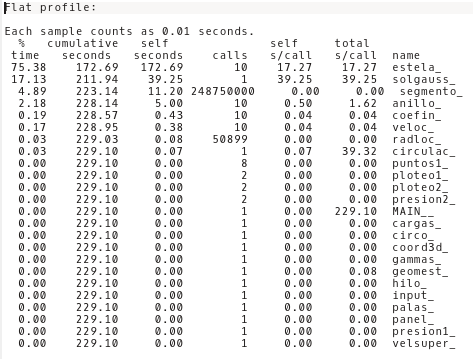
\includegraphics[width=0.60\textwidth]{figuras/gprof3.png} \\
  \caption{Resultado de \emph{gprof} en el c\'odigo optimizado serialmente.} %
   \label{figGprofInt}
\end{figure}


\subsection{An\'alisis de la subrutina Estela}

En la definici\'on de la subrutina ``estela'', el c\'odigo documentado del programa indica que \'esta realiza ``c\'alculo de los coeficientes de influencia de los hilos libres''. Los c\'alculos realizados dentro de la subrutina son numerosos y complejos, por lo cual utilizaremos un pseudoc\'odigo para poder observar los puntos m\'as importantes dentro de la subrutina que pueden ser candidatos a ser paralelizados. En la Fig. \ref{codEstela} aparece el pseudoc\'odigo anotado de la subrutina estela.

\begin{figure}[htbp]
   \begin{lstlisting}[style=consola]
    subrutina estela()
    definicion variables globales y constantes;

    begin
	Do de i=1 a 2500
	Do de j=1 a 51
		ciex(i,j) = 0
		ciey(i,j) = 0
		ciez(i,j) = 0
	end do
	end do
	%c\'alculos parciales?
	ib = 1

    Do de ir=1 a 2500
    Do de npa=1 a 51
	Do de ik=1 a 2001
		genera fx(ik), fy(ik), fz(ik), dista(ik), denom(ik)
	end do

    # sumatoria terminos impares six, siy, siz
	six,siy,siz = 0
	Do de ik=2 a 2000
		six = six + fx(ik)/denom(ik)
		siy = siy + fy(ik)/denom(ik)
		siz = siz + fz(ik)/denom(ik)
		ik = ik +2
	end do
    # sumatoria terminos pares spx, spy, spz
	spx,spy,spz = 0
	Do de ik=3 a 2000
		spx = spx + fx(ik)/denom(ik)
		spy = spy + fy(ik)/denom(ik)
		spz = spz + fz(ik)/denom(ik)
		ik = ik +2
	end do
	calculo ciex(ir,npa), ciey(ir,npa), ciez(ir,npa)
	if (indice = 1) and (ib = 1) then  ## se ejecuta solo 1 vez
	# calculo coeficientes de la estela x, y, z
		if (i = nr) and (j = nr/2) then  
		# calculo para i=50 y j=25 
		# %nr depende del tama\~no del problema,?
		# %en este caso el tama\~no es 50?
			inicializa valx,valy,valz
			Do de ik=1 a 2001
				escribe archivo integ1.txt con varios valores incluyendo valx,valy,valz
				if (ik =/= 2001) then
					const=1
					if (ik == 2000) then
						const=0.5
					endif
					valx = valx + fx(ik+1)/denom(ik+1)*otros valores
					valy = valy + fy(ik+1)/denom(ik+1)*otros valores
					valz = valz + fz(ik+1)/denom(ik+1)*otros valores
				else 
					escribe integ1.txt con varios valores sin valx,valy,valz 
					pero con ciex,ciey,ciez(i,j)
				endif
		else
			if (i = nr/2) and (j = nr+1) then 
			# Luego (si no entr\'o en el anterior if) el calculo es para i = 25 y j=51
				Repite mismo trabajo pero escribiendo integ2.txt
			endif
		endif
	endif
    end do
    end do
    end
  \end{lstlisting}
  \caption{Pseudoc\'odigo de la subrutina \emph{estela}.}
  \label{codEstela}
\end{figure}

Analizando el pseudoc\'odigo podemos observar que la subrutina tiene partes bien diferenciadas. Un inicio, estableciendo valores iniciales y c\'alculos parciales, y luego un bloque conformado por dos bucles principales; dentro de ellos es donde se encuentran las estructuras que pueden ser paralelizadas.

El bucle inicial calcula los datos en fx, fy, fz, denom y dista; luego calcula t\'erminos pares e impares, y finaliza con el denominado c\'alculo de coeficientes de la estela x,y,z. 

El c\'alculo de coeficientes parece ser el m\'as complejo de los puntos indicados, pero si observamos bien, s\'olo se ejecuta una vez en todo el programa, cuando ``indice'' es igual a 1 (la variable ``ib'' siempre tiene valor 1, por lo cual no la contamos). Dicha variable ``indice'' es global al programa y controla las etapas por las que pasa, toma valores de 1 a 10 y no repite los valores.

Por otra parte, el c\'alculo de coeficientes se hace sobre los valores valx, valy y valz, realizando sobre ellos una sumatoria, con lo cual se crea una dependencia de datos entre el c\'alculo de un valor y los c\'alculos previos (cap\'itulo 2 OpenMP), ya que para obtener el valor de valx en un momento, es necesario el valor previo de valx. Si realizamos una paralelizaci\'on del c\'odigo tendr\'iamos un problema en los l\'imites de los distintos threads. 

Por ejemplo, al dividir los datos en porciones de 100 elementos, el thread que calcula los valores 101 a 200 de un bucle necesita conocer el valor de la sumatoria en el valor 100 para poder iniciar con valores correctos su c\'alculo, y dicho valor 100 puede no existir a\'un en el momento en que se lo necesita (porque el thread encargado de su c\'alculo puede no haber finalizado o siquiera iniciado).

En el c\'alculo de los t\'erminos pares e impares se presenta el mismo problema de dependencias de datos que aparece en el c\'alculo de coeficientes. Cuando calculamos, por ejemplo, six, necesitamos conocer el valor previo de six en ese momento.

Existen t\'ecnicas y formas de transformar el c\'odigo que permiten en algunos casos poder reprogramar una porci\'on de c\'odigo para que pueda ser paralelizable a pesar de tener estas dependencias de datos. Debido al potencial gran cambio necesario en el c\'odigo para subsanar el problema de la dependencia de datos, y al requisito de no modificar el c\'odigo de maneras que puedan volverlo ilegible para el usuario, es que no se avanz\'o sobre estas \'areas de la subrutina. La soluci\'on a este problema puede ser motivo de un trabajo futuro que se pondr\'a a consideraci\'on en el cap\'itulo 5.

Luego de descartar estos puntos como las zonas a paralelizar en la subrutina ``estela'' nos quedamos con el bucle de la Fig. \ref{codEstela} que genera los arrays fx, fy, fz, denom y dista (lineas 17 a 19), ya que cada valor generado de estos arrays no depende de otros previos dentro de los arrays.

\subsection{Optimizaci\'on con OpenMP de subrutina Estela}
Seleccionado el bucle a paralelizar hicimos un an\'alisis de los datos que intervienen para poder realizar una optimizaci\'on correcta. Realizamos varias pruebas para definir las directivas OpenMP correctas, quedando definido un conjunto de datos que debe ser compartido por cada thread lanzado por OpenMP y ciertas variables que deben ser privadas de cada uno de ellos.

El bloque de c\'odigo seleccionado para optimizar es el siguiente (ha sido abreviado):
\begin{lstlisting}[style=For]
   do 3 ik=1,kult
   fx(ik)=[calculo con valores de varias matrices]
   fy(ik)=[calculo con valores de varias matrices]
   fz(ik)=[calculo con valores de varias matrices]
   fz(ik)=(-1.)*fz(ik)
   dist2=[calculo con valores de varias matrices]
   dista(ik)=dsqrt(dist2)                                  
   denom(ik)=dista(ik)**3                   
3 continue
\end{lstlisting}
Este bucle es el primer bucle interno de dos iteraciones mayores que incluyen m\'as c\'alculos con otras estructuras, las cuales dependen de los resultados obtenidos en este primer bucle.

Se calculan tres arrays llamados fx, fy y fz, un valor dist2, y dos arrays m\'as basados en el valor de dist2, llamados dista y denom.

Los c\'alculos de los tres primeros arrays y del valor dist2 dependen de varios otros arrays ya calculados previamente, y que la subrutina obtiene por el \'area de datos com\'un con el resto de partes del programa Fortran, adem\'as de utilizar funciones propias del lenguaje.

En un primer an\'alisis del bloque de c\'odigo observamos una posible dependencia de datos en las l\'ineas (5) y (8) del c\'odigo anterior. En la primera, el c\'alculo de fz(ik) depende de s\'i mismo y en la segunda el valor de denom(ik) depende del valor de dista(ik) que depende de dist2. Si bien es posible que no surgieran problemas con estos valores, para evitar resultados inesperados, decidimos analizar y modificar si fuera necesario para evitar la dependencia, siempre que el cambio no fuera significativo, como reescribir la estructura de control completa o varias l\'ineas con nuevas instrucciones.

La dependencia de datos en la l\'inea (5) pudo solucionarse r\'apida y elegantemente. La l\'inea multiplica el valor en fz(ik) por -1, por lo cual es posible agregar este c\'alculo al final de la l\'inea (4) quedando de la siguiente manera:
\begin{lstlisting}[style=For, numbers=none]
  fz(ik)=([c\'alculo con valores de varias matrices])*(-1.)
\end{lstlisting}
En el caso de la l\'inea (8) el an\'alisis es distinto: la dependencia se encuentra en el valor de dista(ik) el cual es calculado en el paso previo y depende del c\'alculo del valor dist2. Adem\'as, se trata de un c\'alculo simple con una funci\'on interna del lenguaje Fortran. Se podr\'ia utilizar un c\'alculo intermedio y luego asignar el resultado a dista(ik) y denom(ik), por ejemplo:
\begin{lstlisting}[style=For, numbers=none]
  var_aux = dsqrt(dist2)
  dista(ik) = var_aux
  denom(ik) = var_aux**3
\end{lstlisting}
Pero enfrentamos la indeterminaci\'on del valor inicial de var\_aux, y c\'omo afecta a cada bloque paralelo cuando realicemos la optimizaci\'on con OpenMP. Esto se puede resolver llevando un control de la variable en el bloque declarativo de OpenMP e inicializando la variable cada vez que es utilizada, lo que agrega carga de control al bloque de c\'odigo (tanto en OpenMP como en el c\'odigo Fortran normal). Si el c\'alculo a realizar con dist2 fuera de mayor complejidad podr\'ia justificarse la utilizaci\'on de una variable auxiliar intermedia, pero como es un c\'alculo sencillo que utiliza una funci\'on interna de Fortran a la cual se le env\'ia un solo valor, se puede resolver de la siguiente manera:
\begin{lstlisting}[style=For, numbers=none]
    dista(ik) = dsqrt(dist2)
    denom(ik) = (dsqrt(dist2))**3
\end{lstlisting}
Se puede entender mejor la dependencia de datos y la necesidad de controlar ciertas variables en los bloques paralelizados al observar un problema importante que surgi\'o durante el trabajo de tesis, el cual incluso no estaba a simple vista. 

Al realizar la optimizaci\'on paralela los resultados del programa eran distintos a los de la ejecuci\'on normal. Los resultados deben ser iguales, dado que el programa es completamente determin\'istico; por lo cual se buscaron muchas formas diferentes con directivas de OpenMP de controlar la ejecuci\'on de los threads en este bloque seleccionado para optimizaci\'on, para que los datos no se contaminaran, pero siempre arribando al mismo resultado err\'oneo. 

El problema se encontr\'o en otra porci\'on de c\'odigo que parec\'ia bastante simple de paralelizar y sin necesidad de control alguno. Al iniciar, la subrutina estela utiliza dos estructuras DO anidadas que inicializan con valor 0 tres arrays (ciex, ciey y ciez), por lo cual con una estructura OMP PARALLEL DO de OpenMP deber\'ia bastar para paralelizar el c\'alculo y obtener una mejora, si bien poco considerable, en performance.

El problema surge porque la inicializaci\'on a 0 se realiza a trav\'es de una variable llamada ``cero'' definida en otra parte del c\'odigo con el valor 0. Al lanzarse los threads de OpenMP dicha variable pas\'o a tener un valor indeterminado para cada thread, trayendo consigo datos espurios a los c\'alculos siguientes donde los arrays intervienen. Al comentar las directivas OpenMP que encerraban dichos bloques DO los resultados del programa volvieron a ser correctos.

Si bien el comportamiento por defecto de OpenMP deber\'ia ser compartir entre todos los threads las variables en memoria del programa principal, no ocurri\'o en este caso con la variable ``cero'', y no se encontr\'o una explicaci\'on para este hecho. Investigar estas particularidades, c\'omo una implementaci\'on del est\'andar OpenMP difiere de otras, y qu\'e problemas acarrean estas diferencias, puede ser motivo de una extensi\'on futura de este trabajo de tesis.  %OSO ESTO ES ASI NOMAS CHE? %HANDRU si, se quita la parte openmp y anda ok, lo arm\'e con control sobre la variable "cero" y anduvo ok, pero no lo agregue al trabajo. 

Con las modificaciones indicadas el bucle ya estaba en condiciones de ser paralelizado con OpenMP.

Lo primero que realizamos, como se planific\'o en el cap\'itulo 2, es indicar el comienzo de la regi\'on paralela y su final:
\begin{lstlisting}[style=For, numbers=none]
!$OMP PARALLEL
[bucle paralelizado]
!$OMP END PARALLEL
\end{lstlisting}
Ahora deb\'iamos agregar las directivas para indicar que la regi\'on paralela deb\'ia ser una estructura DO, por lo que agregamos las directivas DO de OpenMP:
\begin{lstlisting}[style=For, numbers=none]
!$OMP PARALLEL
!$OMP DO

[bucle paralelizado]

!$OMP END DO
!$OMP END PARALLEL
\end{lstlisting}
Al realizar estos cambios en el c\'odigo para el bloque indicado, conseguimos una gran mejora en el tiempo empleado, pero los resultados a\'un no eran correctos. Teniendo en cuenta esto debemos considerar qu\'e variables son compartidas por los distintos threads del proceso y cu\'al es su alcance, para evitar discrepancias en los resultados.

En el bloque de c\'odigo observamos que para realizar el c\'alculo de los arrays son necesarios varios otros arrays y variables, los que ya poseen valores previos. Adem\'as utiliza las variables de control ir y npa de los bloques DO exteriores donde est\'a anidado nuestro bloque de c\'odigo, utilizadas para recorrer los arrays indicados en la Fig. \ref{codEstela}. Podemos ver esto en la tabla \ref{tab:tabVar}.

\begin{table}[htb]
\begin{center}
\begin{tabular}{|c|c|}
\hline 
\rule[-1ex]{0pt}{2.5ex} Tipo Variable & Variables \\ 
\hline 
\hline
\rule[-1ex]{0pt}{2.5ex}  & pcx, pcy, pcz \\
\rule[-1ex]{0pt}{2.5ex} Arrays & xe, ye, ze \\
\rule[-1ex]{0pt}{2.5ex}  & re, fi \\
\hline
\rule[-1ex]{0pt}{2.5ex} Variable float & c0 \\
\hline
\rule[-1ex]{0pt}{2.5ex} Variables de control & ir, npa \\
\hline
\end{tabular} 
\caption{Variables necesarias para el c\'odigo paralelizado.}
\label{tab:tabVar}
\end{center}
\end{table}

El primer interrogante era saber si los datos se deben compartir entre todos los threads o deben ser privados. Si observamos todos los arrays y variables externos que se utilizan para el c\'alculo, los threads deben compartir su valor; si los defini\'eramos como PRIVATE su valor ser\'ia indefinido para cada thread, y si fuera como FIRSTPRIVATE aun cuando los valores fueran correctos, la cantidad de recursos necesarios para la ejecuci\'on se multiplicar\'ia por la cantidad de threads que estuvieran en ejecuci\'on, ya que cada uno tendr\'ia una copia de cada variable. 

Luego, los arrays modificados dentro del bloque son escritos por cada thread, pero cada thread accede a las posiciones definidas por la variable de control del bloque DO que estamos paralelizando, ik, la cual tendr\'a un valor para cada thread espec\'ifico; por ejemplo si dividimos un DO de 100 iteraciones en 2 threads, la variable de control ik tendr\'a valor inicial de 0 para un thread y 50 para el otro.

Esto nos lleva a que los arrays modificados dentro del bloque tambi\'en puedan ser compartidos por todos los threads, ya que s\'olo son accedidos indexados por la variable ik la cual, como indicamos, ser\'a distinta para cada thread, con lo cual cada uno acceder\'a a modificar posiciones de los arrays distintas.

Por todo esto, concluimos que la gran mayor\'ia de arrays y variables son compartidas por todos los threads, y la dependencia de datos entre \'estos es inexistente (los arrays escritos no son le\'idos, los arrays y variables le\'idas no son modificadas), con lo cual definimos en la instrucci\'on OpenMP de inicio del bloque paralelo como DEFAULT(SHARED) para todas las variables utilizadas dentro. Si bien \'este es el comportamiento por defecto que asume el est\'andar OpenMP, lo dejamos declarado expl\'icitamente, no s\'olo por legibilidad, sino para evitar que una eventual implementaci\'on de OpenMP de un compilador genere resultados incorrectos, por ejemplo como ocurre con la variable ``cero'' que vimos en el problema explicado previamente en esta misma secci\'on. Definimos entoncs el bloque de c\'odigo paralelo de la siguiente manera: %OSO SE ACLARO AL DESCRIBIR OPENMP QUE ES POSIBLE UNA ELECCION DE SHARING DEFAULT? HANDRU EST\'a ACLARADO
\begin{lstlisting}[style=For, numbers=none]
!$OMP PARALLEL DEFAULT(SHARED)
!$OMP DO

[bucle paralelizado]

!$OMP END DO
!$OMP END PARALLEL
\end{lstlisting}
Con esta definici\'on tenemos que todas las variables (arrays y variables comunes) ser\'an compartidas por todos los threads. 

En un siguiente nivel de an\'alisis, vemos que hay variables que necesitan definirse privadas de cada thread, principalmente la variable dist2 que es calculada dentro de cada thread en cada una de las iteraciones. Si fuera una variable compartida, todos los threads escribir\'ian en ella en orden impredecible, llevando a resultados err\'oneos. S\'olo para ejemplificar, supongamos que el thread 1 calcula la variable dist2 en una iteraci\'on, luego escribe el valor de dista(ik) con dist2; en ese momento el thread 4 calcula y escribe dist2. Cuando el thread 1 va a escribir el valor de denom(ik), dist2 ya tiene un valor completamente distinto al que hab\'ia calculado el thread 1 previamente. Por esto declaramos a dist2 como PRIVATE.

Para evitar un problema similar al de la variable ``cero'' decidimos declarar las variables de control ir y npa, y la variable ncapa como FIRSTPRIVATE, de manera que sean privadas de cada thread y tengan desde el principio su valor original. El c\'odigo resultante es el siguiente:
\begin{lstlisting}[style=For, numbers=none]
!$OMP PARALLEL DEFAULT(SHARED)
!$OMP DO FIRSTPRIVATE(ir,npa,ncapa) PRIVATE(dist2)

[bucle paralelizado]

!$OMP END DO
!$OMP END PARALLEL
\end{lstlisting}
Luego de estos cambios, la ejecuci\'on del nuevo c\'odigo dio resultados correctos comparados con la ejecuci\'on original. De esta manera paralelizamos parte del bloque de c\'odigo que m\'as tiempo consum\'ia de toda la aplicaci\'on. En el cap\'itulo 4 consideraremos la comparaci\'on de tiempos obtenidos para cada uno de los c\'odigos y soluciones a peque�os contratiempos encontrados.

\label{pagcap4}
\chapter{Pruebas de ejecuci\'on}

\section{Introducci�n}

En este capitulo se presentan los resultados obtenidos en cada etapa de la optimizaci\'on, especialmente el speedup de la aplicaci\'on pero tambi\'en mostrando el uso de archivos en disco as\'i como la cantidad de memoria necesaria. Se mostrar\'a tambi\'en el estado del sistema durante las distintas ejecuciones de la aplicaci\'on.
Como la optimizaci\'on se realiz\'o en varios pasos se mostraran los resultados iniciales, parciales y finales del proceso. De esta manera es posible ver el impacto de cada parte de la optimizaci\'on en el c\'odigo legacy. Como indican \citep[Cap. 2]{Grama} la optimizaci\'on previa del c\'odigo serial es necesaria para evitar efectos indeseados en las mediciones, y puede representar un factor de speedup de la aplicaci\'on de entre 2X y 5X. 
La aplicaci\'on fue modificada lo menos posible en el proceso de optimizaci\'on por lo cual no toda la ganancia posible en una recodificaci\'on es alcanzada, pero como se explic\'o en el capitulo anterior, se trat\'o de hacer los cambios lo mas transparente posibles al usuario y creador de la aplicaci\'on.
El c\'odigo de la aplicaci\'on objeto de estudio de esta tesis es entregado junto con los resultados generados para dos conjuntos de datos de entrada, uno para un n\'umero total de paneles de 50x50 y otra para un n\'umero total de 80x80, siendo estos valores definidos en un archivo que sirve de entrada de datos. Para este trabajo de tesis se elige trabajar principalmente con el conjunto de datos resultante del caso de cantidad de paneles 50x50, sin embargo se presentan observaciones obtenidas de una prueba en uno solo de los equipos para el caso de tama\~no 80x80. El usuario y creador de la aplicaci\'on indic\'o que la ejecuci\'on de la aplicaci\'on con el tama\~no del problema en 50x50 paneles demoraba en el orden de horas de ejecuci\'on, indicando que se dejaba corriendo de un d\'ia para el otro. El tama\~no de 80x80 pod\'ia llegar a durar d\'ias. No se tienen datos fehacientes de estas ejecuciones, las cuales eran realizadas en computadoras de mediados de la d\'ecada del 90.

\section{Equipos/Computadoras/Arquitecturas de prueba}

Las pruebas se llevaron a cabo en dos equipos para obtener resultados que permitieran realizar una mejor evaluaci\'on del proceso de optimizaci\'on. 
Las computadoras utilizadas fueron una PC y una Notebook, ambas multiprocesador y con arquitectura de 64 bits. A continuaci\'on la descripci\'on de los equipos: 
\begin{itemize}
\item Equipo 1 (PC Clon):
     \begin{itemize}
      \item Procesador AMD Phenom II x4 955 x86\_64
            \begin{itemize}
             \item 4 n�cleos reales.
             \item Frecuencia m\'axima de 3.2 Ghz.
             \item Release date: Abril del 2009.
            \end{itemize}
      \item Mother ASUS M4A785TD-V EVO
      \item 4Gb RAM DDR3 1333Mhz.
      \item HD SATA II 3Gbps.
      \item USB 2.0 (480 Mbps)
     \end{itemize}
\end{itemize}
\begin{itemize}
\item Equipo 2 (Notebook):
      \begin{itemize}      
      \item Procesador Intel Core i3-370M x86\_64
             \begin{itemize}
             \item 2 n�cleos reales + 2 hilos de control por n�cleo.
             \item Frecuencia m\'axima de 2.4 Ghz
             \item Release date: Junio del 2010.
             \end{itemize}
      \item Mother Dell 0PJTXT-A11.
      \item 6Gb RAM DDR3 1333Mhz.
      \item HD SATA II 3Gbps.
      \item USB 2.0 (480 Mbps)
      \end{itemize}
\end{itemize}

Nos referiremos en adelante al primer equipo como PC1 y al segundo equipo como PC2.
Se utiliz\'o una versi\'on Live USB de Slackware Linux como sistema operativo para las pruebas. Como disco de almacenamiento sobre el que corr\'ia la aplicaci\'on se utiliz\'o un Flash Drive USB, en el cual se crearon los archivos durante la ejecuci\'on.
Una nota sobre la arquitectura del procesador de PC2. En este caso el procesador tiene dos n\'ucleos, pero al ofrecer dos hilos de control por n\'ucleo, el sistema operativo los ve como si tuviera disponibles cuatro n\'ucleos. El procesador luego distribuye los recursos disponibles sobre cada hilo de acuerdo a lo solicitado por el sistema operativo.

\section{Pruebas de tiempo}
Para las pruebas de tiempo se utiliz\'o el comando \emph{time}\footnote{Para una referencia del comando en GNU/Linux ver su manpage: ``man 1 time''.} de manera de poder evaluar el tiempo real consumido por la aplicaci\'on en sus diferentes etapas: programa original, optimizado serialmente, optimizado paralelamente. Mostraremos los tiempos en los equipos seleccionados para las pruebas y las mejoras en desempe\~no que obtuvimos en el programa en cada iteraci\'on de la optimizaci\'on. El tama\~no de programa seleccionado para las pruebas generales es de 50x50 paneles, el mas peque\~no provisto por el usuario de la aplicaci\'on.
Tambi\'en se incluyen muestras del estado de los archivos en disco luego de la ejecuci\'on del programa, el estado de la memoria y la CPU en plena ejecuci\'on del programa, para mostrar los resultados de las optimizaciones realizadas.
\subsection{Estado inicial y primeras mediciones}
Como se indic\'o previamente, s\'olo contamos con el c\'odigo original y los datos de resultados provistos por el usuario de la aplicaci\'on. Lo primero que hicimos fue compilar y ejecutar el programa original para calcular el tiempo inicial de referencia para el resto del trabajo, resguardando de una posible reescritura a los datos originales, que luego utilizaremos para poder verificar la correctitud de las distintas versiones del proceso de optimizaci\'on. 
En ambos equipos realizamos la compilaci\'on con el siguiente comando:
\begin{lstlisting}[style=consola, numbers=none]
   $ gfortran -o serial invisidos2fin.for
\end{lstlisting}
Esto crea un archivo ejecutable llamado ``serial''.
Para poder lanzar el ejecutable y poder verificar el tiempo lo realizamos con el comando:
\begin{lstlisting}[style=consola, numbers=none]
   $ time ./original
\end{lstlisting}
El tiempo resultante calculado por el comando ``time'' (Fig. \ref{figTSerial}) arroja para la linea ``real'' (tiempo real/total de ejecuci\'on) 21m48.109s para el equipo PC1. El equipo PC2 muestra un tiempo de 22m56.392s. 

Podemos observar que con un cambio en la arquitecura del procesador (PC1 con 4 n�cleos reales, PC2 con 2 n�cleos y 2 hilos de control por n�cleo) se incurre en una demora de 1m8s. Se tom\'o otra muestra con el equipo PC2 y se obtuvo un resultado similar, 23m1.628s por lo que podr\'iamos indicar que la diferencia persiste y se mantiene dentro de ciertos par\'ametros. Esta diferencia observada se debe posiblemente a la mayor velocidad del procesador en PC1. Ser\'ia de inter\'es investigar el uso de la jerarqu\'ia de memoria, especialmente de las caches, en ambos procesadores.
\begin{figure}[t!]
 \centering
    \begin{subfigure}[t]{0.4\linewidth}
    \centering
		\begin{lstlisting}[style=consola, numbers=none]
    real    21m48.109s 
    user    19m3.067s
    sys     0m29.685s
    live@PC1 $ 
		\end{lstlisting}
	\caption{Equipo PC1}
	\end{subfigure}%
	\hspace{.5cm}%
    \begin{subfigure}[t]{0.4\linewidth}
    \centering
		\begin{lstlisting}[style=consola, numbers=none]
    real    22m56.392s 
    user    20m7.858s
    sys     0m32.917s
    live@PC2 $ 
		\end{lstlisting}
	\caption{Equipo PC2}
	\end{subfigure}
\caption{Tiempo de la versi�n serial original.}
\label{figTSerial}
\end{figure}

La ejecuci\'on genera todos los archivos utilizados para c\'alculos intermedios y resultados finales as\'i como los temporales con los que el programa trabaja. 
La ejecuci\'on serial del programa original gener\'o en ambos equipos la misma cantidad de archivos, 58 archivos (Fig. \ref{figListS}) entre los ``.txt'', ``.plt'', ``.out'' y los ``.tmp'', esto es as\'i por el determinismo del programa. No contamos el archivo ejecutable ni el de datos de ingreso ``entvis2f.in''. 
El tama\~no en disco ocupado tanto en PC1 como en PC2 por los archivos fue de 684 Mb (Fig. \ref{figListS}), donde el mayor tama\~no era ocupado por los ocho archivos ``.tmp'', de los cuales siete ocupan 96 Mb cada uno para un total de 672 Mb. 
\begin{figure}[htb]%[htp]
\centering
  \begin{subfigure}[t]{1\linewidth}
  \centering
  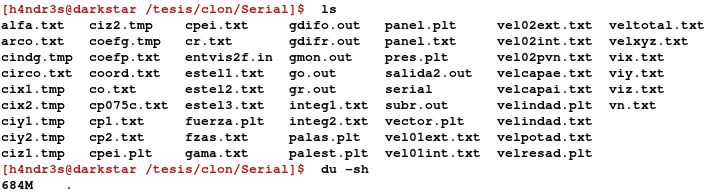
\includegraphics[width=0.80\textwidth]{figuras/clon-serial-arch-du.png} \\
  \caption{PC1}
  \end{subfigure}
  \begin{subfigure}[b]{1\linewidth}
  \centering
  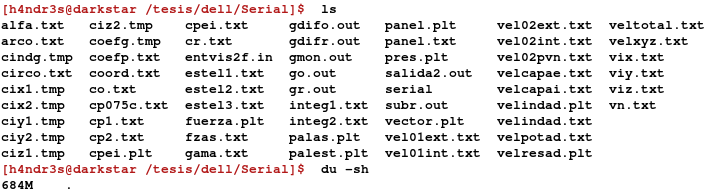
\includegraphics[width=0.80\textwidth]{figuras/dell-serial-arch-du.png} \\
  \caption{PC2}
  \end{subfigure}
\caption{Original: List. de archivos y tama�o del directorio por equipo.} 
\label{figListS}
\end{figure}

La cantidad de memoria consumida por el programa al iniciar en cada equipo es de 217 MB en PC1 y lo mismo en PC2. Cuando durante la ejecuci\'on la aplicaci\'on ingresa en la subrutina solgauss la memoria se incrementa a 255 MB. Y al salir de esta subrutina la memoria baja a 217 MB. Esto nuevamente en ambos equipos. La salida por pantalla de la aplicaci\'on nos permite saber en que subrutina se encuentra, por ello en tiempo de ejecuci\'on podemos determinar estos estados de la memoria. Justamente la rutina solgauss representa un pico en la cantidad de memoria consumida por la aplicaci\'on.
Estos datos se obtienen del comando \emph{pmap}\footnote{Para una referencia del comando en GNU/Linux ver su manpage: ``man 1 pmap''.} aplicado sobre el proceso en ejecuci\'on, por ejemplo si la aplicaci\'on tiene PID 2228:
\begin{lstlisting}[style=consola, numbers=none]
   $ pmap -x 2228
\end{lstlisting}

\emph{Pmap} reporta informaci�n del mapa de memoria de un proceso, dando en su �ltima l�nea un total en Kbytes de la memoria utilizada (Fig. \ref{figPmap}), importandonos la primer columna donde indica el total de memoria utilizada por el proceso. Por ejemplo en la Fig. \ref{figPmap} vemos el resultado para cada equipo mientras se ejecutaba la aplicaci�n original. El comando ``top'' tambi\'en permite observar el mismo valor que indica ``pmap'' en su columna VIRT.

\begin{figure}[htb]
    \begin{subfigure}[t]{0.5\linewidth}
    \centering
	\begin{lstlisting}[style=consola, numbers=none]
[datos de la aplicaci�n]
------------- ------- ------- -------
total kB      222212  157080  154368
	\end{lstlisting}
	\caption{Equipo PC1}
	\end{subfigure}%
	\hspace{.5cm}%
    \begin{subfigure}[t]{0.5\linewidth}
    \centering
	\begin{lstlisting}[style=consola, numbers=none]
[datos de la aplicaci�n]
------------- ------- ------- -------
total kB      222472  209160  206240
	\end{lstlisting}
	\caption{Equipo PC2}
	\end{subfigure}
\caption{Informaci�n del comando \emph{pmap} en cada equipo.}
\label{figPmap}
\end{figure}

Por \'ultimo la CPU utilizada siempre fue una sola de las disponibles, ya que el programa es serial. Como ejemplo vemos en la Fig. \ref{figTopS} una captura del comando \emph{top} de PC1 durante la ejecuci�n de la aplicaci�n original.

\begin{figure}[htb]%[htp]
  \centering
  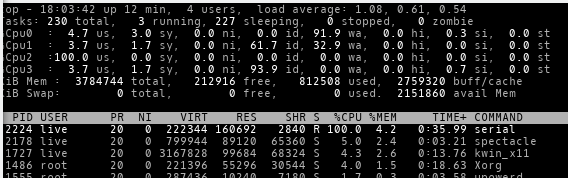
\includegraphics[width=0.80\textwidth]{figuras/clon-top-serial.png} \\
  \caption{Comando \emph{top}: Aplicaci�n original en subrutina ``estla''.} 
   \label{figTopS}
\end{figure}

Los datos vistos hasta el momento en el trabajo de tesis (Tabla \ref{tab:tabDataSerial}), son de la ejecuci\'on del programa original, las dos subsecciones siguientes mostraran como evolucion\'o con la optimizaci\'on, teniendo como base los tiempos y tama\~nos obtenidos en esta primer etapa. 

\begin{table}[htb]
\begin{center}
\begin{tabular}{|l|c|c|}
\hline 
\rule[-1ex]{0pt}{2.5ex}  & PC1 & PC2 \\ 
\hline 
\hline
\rule[-1ex]{0pt}{2.5ex} Archivos generados & 58 & 58 \\
\hline
\rule[-1ex]{0pt}{2.5ex} Esp. en disco utilizado & 684Mb & 684Mb \\
\hline
\rule[-1ex]{0pt}{2.5ex} \multirow{2}{1cm}{Memoria} & Ejecuci�n en \emph{solgauss}: 255Mb & 255Mb \\ \cline{2-3}
& Resto de la ejecuci�n: 217Mb & 217Mb \\ \cline{2-3}
\hline
\rule[-1ex]{0pt}{2.5ex} CPUs utilizadas & 1 & 1 \\
\hline
\rule[-1ex]{0pt}{2.5ex} Tiempo total de ejecuci�n & 21m48s & 22m56s \\
\hline
\end{tabular} 
\caption {Datos de ejecuci�n de la aplicaci�n original en ambos equipos.}
\label{tab:tabDataSerial}
\end{center}
\end{table}

\subsection{Optimizaci\'on serial y mediciones intermedias}
Luego de realizar la optimizaci\'on serial se tomaron nuevamente mediciones. La compilaci\'on se realiz\'o con el mismo comando ya que en esta etapa a\'un no tenemos la adici\'on de ninguna optimizaci\'on paralela.
\begin{lstlisting}[style=consola, numbers=none]
      $ gfortran -o optserial invisidos2fin_optSerial.for
\end{lstlisting}
Y nuevamente para medir el tiempo del programa ejecutamos la aplicaci\'on con la instrucci\'on time.
\begin{lstlisting}[style=consola, numbers=none]
      $ time ./optserial
\end{lstlisting}
El tiempo obtenido en PC1 fue de 16m2.124s, lo que representa una ganancia de 5m36s aproximadamente sobre la versi\'on serial original de la aplicaci\'on en el mismo equipo, teniendo entonces un factor de 1.35 de mejora en el tiempo.
En la computadora PC2 los tiempos obtenidos fueron de 17min 4.161seg. Se observa una mejora sobre la versi\'on serial original de 5m 52s aproximadamente, o un factor de 1.34 de mejora en el tiempo (Fig. \ref{figTIfiles}).

\begin{figure}[t!]
 \centering
    \begin{subfigure}[t]{0.4\linewidth}
    \centering
		\begin{lstlisting}[style=consola, numbers=none]
    real    16m2.124s
    user    16m0.894s
    sys     0m0.259s
    live@PC1 $ 
		\end{lstlisting}
	\caption{Equipo PC1}
	\end{subfigure}%
	\hspace{.5cm}%
    \begin{subfigure}[t]{0.4\linewidth}
    \centering
		\begin{lstlisting}[style=consola, numbers=none]
    real    17m4.161s
    user    17m2.631s
    sys     0m0.428s
    live@PC2 $ 
		\end{lstlisting}
	\caption{Equipo PC2}
	\end{subfigure}
\caption{Tiempo de la versi�n optimizada serialmente.}
\label{figTIfiles}
\end{figure}

Se puede ver que el factor de mejora alcanzado entre el original serial y el optimizado es muy similar entre ambos equipos, con una diferencia de solo 0.01, y que es levemente mejor en PC1.
Estrictamente hablando de los tiempos de ejecuci�n del c\'odigo optimizado serialmente, entre los equipos la diferencia observada es de 1m2s, nuevamente a favor de PC1.

Al observar el directorio donde se ejecuta la aplicaci\'on, observamos que luego de la optimizaci\'on serial han desaparecido los archivos ``.tmp'' (Fig. \ref{figListI}), ya que ahora lleva los c\'alculos intermedios en la memoria para poder mejorar los tiempos de acceso. El resto de archivos (50 en total) siguen creandose, pero al demorar la escritura de los archivos utilizados para ir mostrando y almacenando la salida por pantalla, tanto como los que son leidos y escritos y obtienen resultados finales, se logra evitar el acceso constante al disco a trav\'es de la ejecuci\'on de la aplicaci\'on, para tener solo que hacerlo una vez por archivo al finalizar la ejecuci\'on del programa o una subrutina en particular.
El tama\~no ocupado por los archivos del programa ahora fue de 17 Mb tanto en PC1 como en PC2 (Fig. \ref{figListI}), observando nuevamente el impacto de no generar los archivos ``.tmp''. 

\begin{figure}[h]%[htp]
  \centering
  \begin{subfigure}[t]{1\linewidth}
  \centering
  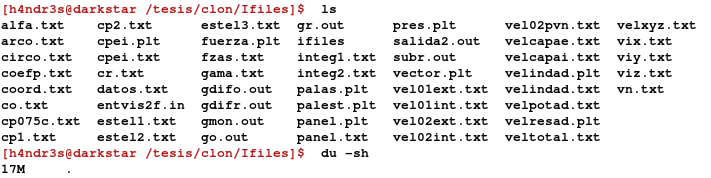
\includegraphics[width=0.80\textwidth]{figuras/clon-ifiles-arch-du.png} \\
  \caption{PC1}
  \end{subfigure}
  \begin{subfigure}[b]{1\linewidth}
  \centering
  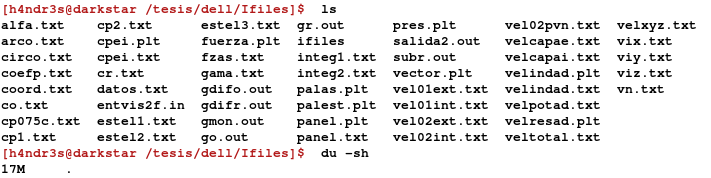
\includegraphics[width=0.80\textwidth]{figuras/dell-ifiles-arch-du.png} \\
  \caption{PC2}
  \end{subfigure}
\caption{Opt. Serial: List. de archivos y tama�o del directorio por equipo.} 
\label{figListI}
\end{figure}

Observando la memoria en esta versi\'on del programa obtenemos que consume 552 Mb mientras est\'a en solgauss y 504MB el resto del tiempo, tanto en PC1 como PC2 (Fig. \ref{figPmapI}). Esto significa un incremento en la cantidad de memoria utilizada, en esta versi\'on optimizada serialmente con respecto a la versi\'on serial original, de 297MB cuando el programa est\'a en la subrutina solgauss y de 287MB antes o despu\'es de dicha subrutina. Este incremento se debe a los archivos ``.tmp'' que ya no utiliza mas en disco y debe llevar en memoria como internal files. 

\begin{figure}[htb]
    \begin{subfigure}[t]{0.5\linewidth}
    \centering
	\begin{lstlisting}[style=consola, numbers=none]
[datos de la aplicaci�n]
------------- ------- ------- -------
total kB      516392  504060  501276
	\end{lstlisting}
	\caption{Equipo PC1}
	\end{subfigure}%
	\hspace{.5cm}%
    \begin{subfigure}[t]{0.5\linewidth}
    \centering
	\begin{lstlisting}[style=consola, numbers=none]
[datos de la aplicaci�n]
------------- ------- ------- -------
total kB      516524  504308  501332
	\end{lstlisting}
	\caption{Equipo PC2}
	\end{subfigure}
\caption{Comando \emph{pmap} con la aplicaci�n optimizada serialmente (fuera de ``solgauss'').}
\label{figPmapI}
\end{figure}

\begin{table}[htb]
\begin{center}
\begin{tabular}{|l|c|c|}
\hline 
\rule[-1ex]{0pt}{2.5ex}  & PC1 & PC2 \\ 
\hline 
\hline
\rule[-1ex]{0pt}{2.5ex} Archivos generados & 50 & 50 \\
\hline
\rule[-1ex]{0pt}{2.5ex} Esp. en disco utilizado & 17Mb & 17Mb \\
\hline
\rule[-1ex]{0pt}{2.5ex} \multirow{2}{1cm}{Memoria} & Ejecuci�n en \emph{solgauss}: 552Mb & 552Mb \\ \cline{2-3}
& Resto de la ejecuci�n: 504Mb & 504Mb \\ \cline{2-3}
\hline
\rule[-1ex]{0pt}{2.5ex} CPUs utilizadas & 1 & 1 \\
\hline
\rule[-1ex]{0pt}{2.5ex} Tiempo total de ejecuci�n & 16m02s & 17m04s \\
\hline
\end{tabular} 
\caption {Datos de ejecuci�n de la aplicaci�n optimizada serialmente.}
\label{tab:tabDataIfiles}
\end{center}
\end{table}

Nuevamente en el caso de la CPU podemos observar que un solo procesador es el encargado de realizar la tarea ya que a\'un no se optimiza paralelamente. En la Fig. \ref{figTopI} podemos observar como ejemplo, la ejecuci\'on de la aplicaci\'on optimizada serialmente en PC1, en el momento que est\'a dentro de la subrutina estela.

\begin{figure}[htb]%[htp]
  \centering
  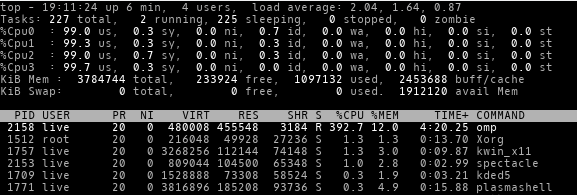
\includegraphics[width=0.80\textwidth]{figuras/clon-top-omp.png} \\
  \caption{Comando \emph{top}: Aplicaci�n opt. serialmente en subrutina ``estela''.} 
   \label{figTopI}
\end{figure}

La Tabla \ref{tab:tabDataIfiles} resume la informaci�n obtenida de la optimizaci�n serial de la aplicaci�n. En la siguiente secci�n se ven los resultados de la optimizaci�n paralela mediante OpenMP.

\subsection{Optimizaci\'on Paralela y mediciones finales}

Finalmente realizamos las pruebas con la versi\'on optimizada paralelamente del programa. Para esta prueba cambiamos la forma de compilar el programa ya que se debe indicar que aprovechar\'a las directivas de OpenMP, esto lo realizamos pasando el par\'ametro ``-fopenmp'' al comando de compilaci\'on, de la siguiente manera:
\begin{lstlisting}[style=consola, numbers=none]
   $ gfortran -fopenmp -o paralelo invisidos2fin_optOMP.for
\end{lstlisting}
Al terminar tenemos un ejecutable listo para aprovechar la paralelizaci\'on que brinda OpenMP. 
Nuevamente se ejecut\'o la aplicaci\'on con el comando time, de manera de obtener el tiempo de ejecuci\'on. La ejecuci\'on se hizo sin limitar la cantidad de threads creados en OpenMP, es decir que la aplicaci\'on se ejecut\'o aprovechando todos los threads disponibles por defecto, es decir uno por cada n�cleo disponible (cuatro threads en cada equipo). 
\begin{lstlisting}[style=consola, numbers=none]
   $ time ./paralelo
\end{lstlisting}

Un contratiempo que ocurri\'o en este paso fue que al ingresar en la parte paralelizada, la aplicaci\'on incurri\'o en un error de ``segmentation fault''. El problema ocurre por el tama\~no m\'aximo definido en el kernel Linux de la pila para un proceso, el cual por defecto es de 8192Kb. La soluci\'on es previo a la ejecuci\'on de la aplicaci\'on definir el tama\~no m\'aximo de la pila en ``unlimited'' con el siguiente comando:
\begin{lstlisting}[style=consola, numbers=none]
   $ ulimit -s unlimited
\end{lstlisting}
Luego de establecido el parametro, la ejecuci\'on de la aplicaci\'on es correcta.
 
Los resultados de ``time'' para PC1 indicaron un tiempo de ejecuci\'on de 6m5.294s (Fig. \ref{figTOmp}). Al comparar con los 21m48.109s que tom\'o en su versi\'on original podemos observar 15m42s de mejora aproximada, obteniendo un factor de 3.58 de mejora en el desempe\~no, lo cual es muy superior a la ganancia inicial con la optimizaci\'on serial.
En PC2 obtuvimos 8m50.822s de tiempo de ejecuci\'on (Fig. \ref{figTOmp}), mientras el programa original tom\'o 22m56.392s, es decir aproximadamente 14m6s m\'as r\'apida la versi\'on paralela, obteniendo un factor de 2.59 de mejora en el desempe\~no.
La diferencia de tiempo de ejecuci\'on entre la aplicaci\'on optimizada paralelamente en PC1 y PC2 es de 2m45s, observandose esta vez una diferencia de tiempo considerable.
Se podr\'ia investigar la incidencia de los 4 n�cleos reales del procesador AMD en PC1 contra los 2 n�cleos reales y 2 hilos de control por n�cleo en el procesador Intel de PC2. Ambos procesadores brindan a OpenMP cuatro hilos, pero los recursos son asignados de manera diferente.

\begin{figure}[htb]
 \centering
    \begin{subfigure}[t]{0.4\linewidth}
    \centering
		\begin{lstlisting}[style=consola, numbers=none]
    real    6m5.294s
    user    17m38.896s
    sys     0m0.872s
    live@PC1 $ 
		\end{lstlisting}
	\caption{Equipo PC1}
	\end{subfigure}%
	\hspace{.5cm}%
    \begin{subfigure}[t]{0.4\linewidth}
    \centering
		\begin{lstlisting}[style=consola, numbers=none]
    real    8m50.822s
    user    28m21.227s
    sys     0m4.812s
    live@PC2 $ 
		\end{lstlisting}
	\caption{Equipo PC2}
	\end{subfigure}
\caption{Tiempo de la versi�n optimizada paralelamente con OpenMP.}
\label{figTOmp}
\end{figure}

En el consumo de CPU esta vez podemos observar diferencia entre los programas seriales y uno paralelizado. Se han activado todos los n�cleos disponibles en el equipo al momento de entrar en la zona de la subrutina estela (Fig. \ref{figTopO}), ya sean n�cleos reales (PC1) o virtuales (PC2). 
Como ya indicamos, la activaci\'on de los n�cleos no fue administrada de manera directa con directivas OpenMP por lo cual todos los n�cleos disponibles fueron utilizados, pero como se indicaba en el capitulo 2 hay m\'as directivas que pueden ser estudiadas de OpenMP que podr\'ian ser utilizadas para disminuir o incrementar la cantidad de hilos generados en una regi\'on paralela y estudiar el impacto y la utilizaci\'on de los recursos en el multiprocesador.

\begin{figure}[htb]%[htp]
  \centering
  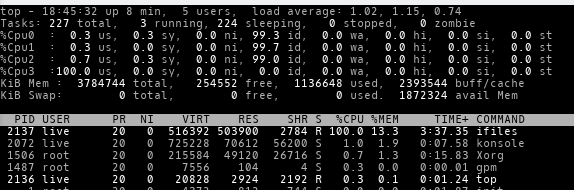
\includegraphics[width=0.80\textwidth]{figuras/clon-top-ifiles.png} \\
  \caption{Comando \emph{top}: Aplicaci�n optimizada con OpenMP en subrutina ``estela''.} 
   \label{figTopO}
\end{figure}

El directorio de ejecuci\'on del programa queda igual que en la versi\'on optimizada serialmente (Ver Fig. \ref{figListI}) ya que en esta nueva versi\'on se han agregado las directivas OpenMP utilizadas y no se ha tocado el c\'odigo serial ni el tratamiento de los archivos. Lo mismo ocurre con el tama\~no ocupado por los archivos en disco (17MB). 

\begin{figure}[htb]
    \begin{subfigure}[t]{0.5\linewidth}
    \centering
	\begin{lstlisting}[style=consola, numbers=none]
[datos de la aplicaci�n]
------------- ------- ------- -------
total kB      480008  455704  452516
	\end{lstlisting}
	\caption{Equipo PC1}
	\end{subfigure}%
	\hspace{.5cm}%
    \begin{subfigure}[t]{0.5\linewidth}
    \centering
	\begin{lstlisting}[style=consola, numbers=none]
[datos de la aplicaci�n]
------------- ------- ------- -------
total kB      480144  455828  452576
	\end{lstlisting}
	\caption{Equipo PC2}
	\end{subfigure}
\caption{Comando \emph{pmap} sobre aplicaci�n optimizada con OpenMP (fuera de ``solgauss'').}
\label{figPmapO}
\end{figure}

Observando la memoria el programa consume 516MB de RAM durante la subrutina solgauss y 468MB en el resto de su ejecuci\'on en ambos equipos (Fig. \ref{figPmapO}). Con respecto al original esto indica un incremento de 261MB de memoria mientras est\'a en solgauss y 251MB en el resto de la ejecuci\'on. Al comparar con la aplicaci\'on optimizada serialmente se observ\'o que el consumo de memoria es menor en la versi\'on con OpenMP. Ocupa 36MB menos durante la ejecuci\'on, tanto si se ejecuta en solgauss como en el resto del tiempo. 
Podr\'ia investigarse esta diferencias en la memoria en la optimizaci\'on que realiza el compilador en el c\'odigo para utilizar las directivas de OpenMP. 

Finalmente podemos ver en la Fig. \ref{figDataTotal} los datos resumidos de las tres versiones de la aplicaci�n.

\begin{figure}[htb]%[htp]
  \centering
  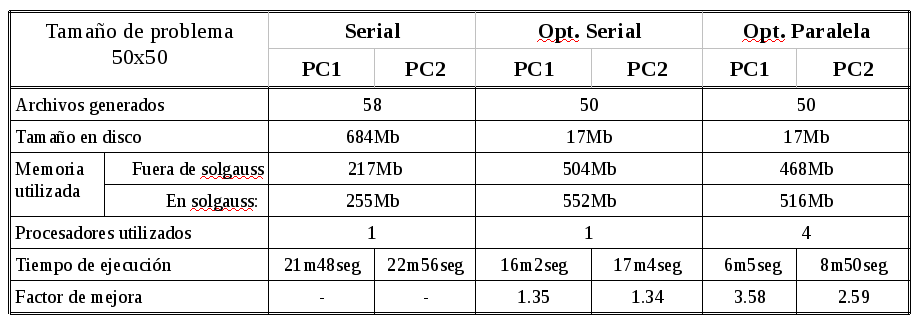
\includegraphics[width=1.0\textwidth]{figuras/tabla-data-final1.png} \\
  \caption{Resumen datos totales de las aplicaciones.} 
   \label{figDataTotal}
\end{figure}

\section{Pruebas con 80x80 paneles}
Para determinar la escalabilidad de la soluci\'on aplicada y como impacta en un equipo el cambio del tama\~no de los datos para el c\'alculo, se realizaron en PC2 pruebas con el segundo tama\~no de prueba provisto por el autor/usuario de la aplicaci\'on, 80x80 paneles.
Solo tenemos los resultados de salida de la ejecuci\'on del original utilizado por el usuario y se utilizaron para verificar los resultados de salida de las versiones utilizadas para la prueba, arrojando que todas dan una salida correcta de los datos.
Como indicamos en el cap\'itulo 3, el archivo con los datos de entrada para la ejecuci\'on de la aplicaci\'on (entvis2f.in) posee una \'unica modificaci\'on con respecto al de 50x50 y que es  nr = no = 80. Luego mediante el an\'alisis de las diferencias entre los c\'odigos de la versi\'on de tama\~no 50x50 contra la de 80x80, observamos que el c\'odigo en los bloques ``common'' de Fortran indica lo siguiente:

\noindent Para el caso 50x50
\begin{lstlisting}[style=For, numbers=none]
   parameter (maxir=51,maxio=51,...
\end{lstlisting}
Para el caso 80x80
\begin{lstlisting}[style=For, numbers=none]
   parameter (maxir=81,maxio=81,...
\end{lstlisting}
Como indicamos en el cap\'itulo 3, maxir y maxio son lo mismo que nr+1 o no+1, lo cual ser\'ia una manera m\'as simple de definirlo. Debido a que la definici�n de estos valores est� fija, literalmente, en cada bloque common de todo el c\'odigo, es que para las optimizaciones, serial y paralela, de la aplicaci\'on con tama\~no de problema 80x80, se debe cambiar en todo el c\'odigo cada una de las definiciones de maxir y maxio.
Luego de adaptado esto procedimos a las pruebas en el mismo orden que antes, versi�n original, versi\'on optimizada serialmente, versi\'on optimizada con OpenMP.

\subsection{Perfilado de aplicaci\'on con tama\~no 80x80}
Previo a correr las pruebas de tiempo en el equipo PC2 realizamos un nuevo an\'alisis de perfilado con la herramienta gprof sobre la aplicaci\'on adaptada a un tama\~no distinto de problema, ya que esto puede afectar el comportamiento de las subrutinas.
Luego de compilar la aplicaci\'on con la opci\'on ``-pg'' activada, la ejecutamos y obtenemos el archivo gmon.out de salida. Con esto podemos generar la informaci\'on del perfilado, el cual indica que la subrutina estela es la que m\'as porcentaje del tiempo se ejecuta seguida de solgauss, pero esta vez los porcentajes cambian completamente. Estela se ejecuta 46,42\% del tiempo mientras que solgauss ahora ocupa un 43,09\% (Fig. \ref{figGprof4}), esto es mucho m\'as que el 14,36\% en PC1 o el 16,84\% en PC2 obtenido por solgauss para la versi\'on de 50x50.
\begin{figure}[htb]%[htp]
  \centering
  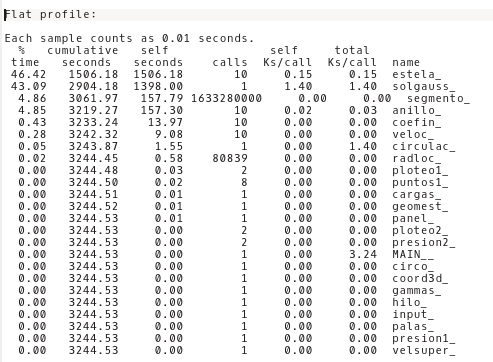
\includegraphics[width=0.60\textwidth]{figuras/gprof4.png} \\
  \caption{Salida de \emph{gprof} para tama�o 80x80.} %
   \label{figGprof4}
\end{figure}

Este cambio que se produce en la ejecuci\'on al agrandar el tama\~no del problema, tendr\'a impacto en los tiempos de las distintas versiones de la aplicaci\'on.

\subsection{Versi\'on serial}
La ejecuci\'on en el equipo PC2 arroj\'o un tiempo de ejecuci\'on de 225m43.721s, es decir 3h45m43s (Fig. \ref{figTS80}). El tama\~no del problema se incrementa de 2500 paneles a 6400 paneles, un incremento de factor 2.56 veces, pero el tiempo se hace exponencial, en un factor de 9.78.

\begin{figure}[htb]
 \centering
	\begin{lstlisting}[style=consola1, numbers=none]
    real    225m43.721s
    user    174m29.803s
    sys     3m11.953s
    live@PC1 $ 
	\end{lstlisting}
\caption{Tiempo de la versi�n original con tama�o 80x80.}
\label{figTS80}
\end{figure}

El espacio en disco utilizado fue de 4415MB o 4.3GB, siendo los archivos ``.tmp'' los que ocupaban 4375MB, siete de los ocho archivos pesando 625MB cada uno. En memoria RAM observamos que la aplicaci\'on llega a ocupar 1293MB o 1.26GB fuera de la subrutina ``solgauss'' y 1581Mb dentro de la subrutina.

\subsection{Versi\'on Optimizada Serialmente}
Los tiempos observados en la versi\'on optimizada del c\'odigo serial son de 150m45.602s, es decir 2h30m45s (Fig. \ref{figTI80}). El factor de incremento esta vez es de 8.83 con respecto a la aplicaci\'on equivalente en el problema de menor tama\~no. Por esto se observa una ganancia de tiempo con respecto a la aplicaci\'on serial de 75m aproximadamente, o un factor de 1.5, el cual es mejor que ante el problema de menor tama\~no. Esto puede ser adjudicado a la mayor cantidad de datos en disco que utiliza la aplicaci\'on con este tama\~no de problema, en comparaci\'on al tama\~no 50x50, que ahora son accedidos en memoria. 

\begin{figure}[htb]
 \centering
	\begin{lstlisting}[style=consola1,numbers=none]
    real    150m45.602s
    user    150m36.178s
    sys     0m3.413s
    live@PC1 $ 
	\end{lstlisting}
\caption{Tiempo de la versi�n optimizada serialmente con tama�o 80x80.}
\label{figTI80}
\end{figure}

En disco se ve claramente el impacto de no utilizar los archivos ``.tmp'' al ocupar solo 40MB.

El incremento, como en la versi\'on de menor tama\~no, se ve en la memoria. Observamos que en ejecuci\'on la aplicaci\'on utiliza mientras est\'a en solgauss 3483MB (3.4GB) y 3171 (3.09GB) en el resto de la ejecuci\'on. El equipo cuenta con 6GB de memoria RAM por lo que no fue necesario que realizara swapping en disco, lo que hubiera impactado en los tiempos.    

\subsection{Versi\'on con optimizaci\'on paralela}
Los tiempos obtenidos en la versi\'on con OpenMP son de 130m39.169s (Fig. \ref{figTOmp80}) o 2h10m39s. Se puede observar en las versiones optimizadas, principalmente por el perfilado con gprof ya mencionado y tambi\'en siguiendo la salida que da el programa por pantalla, que la demora ahora se ubica en la subrutina solgauss. 

\begin{figure}[htb]
 \centering
	\begin{lstlisting}[style=consola1, numbers=none]
    real    130m39.169s
    user    253m34.730s
    sys     0m15.825s
    live@PC1 $ 
	\end{lstlisting}
\caption{Tiempo de la versi�n optimizada paralelamente con tama�o 80x80.}
\label{figTOmp80}
\end{figure}

El tiempo obtenido nos da una mejora que no es igual a la observada en la versi\'on de 50x50, esta vez representa solo una mejora en un factor de 1.73 sobre la aplicaci\'on original.

Si analizamos el tiempo teniendo en cuenta el resultado de gprof para este tama\~no de problema (Fig. \ref{figGprof4}) y para gprof para el tama\~no menor (Fig. \ref{figGprof1} y \ref{figGprof2}) podemos ver que la paralelizaci\'on impacta sobre un 30\% menos de tiempo, limitando la mejora obtenida al incrementar el tama\~no del problema. Esto ocurre porque solo se paraleliza la subrutina ``estela'', siendo que la subrutina ``solgauss'' ahora consume ese 30\% de tiempo. La paralelizaci�n de ``solgauss'' es un posible trabajo futuro.

El comportamiento en disco es exactamente el mismo que en la versi\'on optimizada serialmente, con 40MB de archivos. 
En memoria ocurre igual que en la aplicaci\'on con tama\~no 50x50, ocupando menos que en la versi\'on optimizada serialmente, 3184MB (3.1GB) mientras est\'a en solgauss y 2864MB (2.79GB) en el resto de la ejecuci\'on.

El res�men de los datos totales obtenidos con el tama�o de problema de 80x80 pueden verse en la Fig. \ref{figDataTotal80}.

\begin{figure}[htb]%[htp]
  \centering
  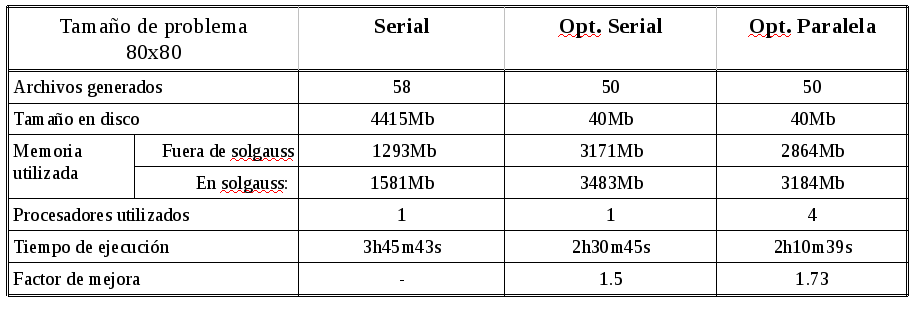
\includegraphics[width=1.0\textwidth]{figuras/tabla-data80-final1.png} \\
  \caption{Resumen datos totales de ejecuci�n 80x80.} 
   \label{figDataTotal80}
\end{figure}

\section{Conclusi\'on}
En este cap\'itulo hemos presentado distintas pruebas de ejecuci\'on de la aplicaci\'on bajo estudio durante el proceso de su optimizaci\'on, distinguiendo tres etapas: aplicaci\'on original, aplicaci\'on optimizada serialmente, aplicaci\'on optimizada paralelamente. 
Adem\'as se utilizaron dos plataformas de hardware distintas para dar mayor amplitud a la prueba y poder observar el comportamiento de la aplicaci\'on con distinto hardware. 
Tambi\'en se realiz\'o una prueba con un tama\~no de problema mayor para ver el impacto de la paralelizaci\'on y se pudo ver el impacto en la memoria RAM, adem\'as de encontrar un perfilado distinto que en la versi\'on de tama\~no de problema menor.\\
Se han podido tomar mediciones de tiempo y de recursos para presentar conclusiones en el siguiente cap\'itulo del trabajo realizado.

Para finalizar se puede afirmar que la aplicaci�n desde su versi�n original hasta la versi�n optimizada y paralelizada resultante de este trabajo de tesis, ha obtenido una mejora en su velocidad de ejecuci�n en un factor de 1.73 en el tama�o de problema mayor (80x80 paneles), y entre 2.59 y 3.58 en su versi�n de menor tama�o (50x50 paneles).


\label{pagcap5}
\chapter{Conclusiones y Trabajos Futuros}

En este cap�tulo se presentan las principales conclusiones de esta tesis. En la �ltima secci�n se presentan las potenciales l�neas futuras de acci�n que puedan complementar el trabajo desarrollado.


\section{Conclusiones}
La paralelizaci�n de una aplicaci�n legacy es una tarea compleja con muchos aspectos. Se realiza en varias etapas incrementales que van impactando en mayor o menor medida en los resultados. La finalidad de la paralelizaci�n puede ser buscar mejorar la performance, la utilizaci�n de recursos, la calidad de los resultados, etc. El presente trabajo se enfoc� en la mejora de utilizaci�n de recursos durante la etapa de optimizaci�n serial, y de la performance en la etapa de optimizaci�n paralela. Sin embargo, en ambas etapas se obtuvieron mejoras parciales en ambos aspectos.

Para poder realizar el trabajo de tesis fue necesario estudiar y aprender el lenguaje Fortran; luego, estudiar el c�digo de la aplicaci�n objeto de estudio para comprender su forma de trabajar, y finalmente poder realizar los cambios necesarios sin modificar substancialmente el c�digo. Recorriendo este camino se adquirieron conocimientos sobre el est�ndar OpenMP y sobre la optimizaci�n de aplicaciones para Computaci�n de Altas Prestaciones.

Para poder enfrentar el trabajo de optimizaci�n adecuadamente fue necesario un an�lisis de la aplicaci�n bajo estudio. Tomamos el programa original, ejecut�ndolo con un tama�o del problema de 50x50, para obtener mediciones que dieran la base de comparaci�n para las etapas de optimizaci�n. Luego se aplic� la optimizaci�n tal como se describi� en el cap�tulo 3: optimizaci�n del c�digo serial en primer lugar, y paralelizaci�n de una porci�n del c�digo posteriormente. Esta paralelizaci�n se realiz� aplicando las directivas de OpenMP a la subrutina estela.

Luego de la primera etapa, de optimizaci�n serial, se logr� una mejora en el tiempo de ejecuci�n, aunque todav�a reducida (factor de mejora o speedup de 1.34). Al realizar la optimizaci�n paralela obtuvimos un mayor speedup (con valores de 3.58 en un equipo de pruebas y 2.59 en otro). Estos factores de mejora estaban m�s de acuerdo con la intuici�n, ya que la optimizaci�n afectaba a una subrutina que consum�a entre un 74\% y un 79\% del tiempo de ejecuci�n original.

Al ocuparnos del uso de discos y memoria, trasladamos los archivos desde el filesystem, residente en disco, a la memoria RAM para un acceso mas r�pido. Sin embargo esta modificaci�n no tuvo un impacto tan notable como se esperaba. Se duplic� aproximadamente la utilizaci�n de memoria RAM, sin que esto representara un inconveniente dados los equipos utilizados. En equipos con 1 GB de RAM (en la actualidad es habitual contar con 2 GB o m�s) el programa seguir�a teniendo memoria suficiente para ejecutarse usando el tama�o de problema de 50x50. 

Por �ltimo, sobre uno de los equipos se llevaron a cabo pruebas con un tama�o de problema mayor (80x80), sobre la versi�n original, optimizada serialmente y optimizada paralelamente. Primero se realiz� un perfilado, donde se pudo observar que los porcentajes de tiempo de las subrutinas estela y solgauss casi se hab�an equiparado (46\% y 43\% respectivamente). En las pruebas esto mostr� que la mejora de tiempo al paralelizar no fue tan grande como con el tama�o de problema menor, lo cual lleva a la necesidad de paralelizar solgauss para poder obtener mayor mejora en tama�os m�s grandes de problema para la aplicaci�n. Tambi�n podemos concluir que claramente el incremento de tama�o del problema y la optimizaci�n impactan en la memoria del sistema y debe tenerse en cuenta la cantidad de RAM disponible si el usuario quisiera incrementar a�n m�s el tama�o del problema.

\section{Trabajos Futuros}
En funci�n del trabajo de tesis se identificaron algunos aspectos que permitir�an extender el trabajo realizado. Estos aspectos se detallan a continuaci�n:
\begin{itemize}
\item Analizar si al aumentar a�n m�s el tama�o del problema, con perfilado de la aplicaci�n original, siguen invirti�ndose los tiempos de las subrutinas, y ver si es necesario optimizar de otra manera. Tambi�n utilizar herramientas de perfilado de aplicaciones paralelas con OpenMP, como ``ompp''.
\item Otra l�nea de trabajo podr�a ser proponer una recodificaci�n de la aplicaci�n para aprovechar mejoras en el lenguaje Fortran y otras bibliotecas existentes para la realizaci�n de los c�lculos.
\item Se podr�a paralelizar la subrutina solgauss y analizar si es necesario recodificar la subrutina o si se puede optimizar en su estado original. Adem�s analizar si la ganancia en performance en el tama�o de problema menor es o no despreciable y en problemas de mayor tama�o, qu� speedup puede obtenerse.
\item Realizar la optimizaci�n utilizando conjuntamente OpenMP y la API MPI, y analizar la posibilidad de utilizar un cluster para la ejecuci�n de la aplicaci�n aprovechando la capacidad de c�mputo de varios nodos.
\item Investigar c�mo una implementaci�n del est�ndar OpenMP difiere de otras y qu� problemas se presentan, teniendo en cuenta el problema visto en el cap 3 con la inicializaci�n en cero de arrays utilizando OpenMP.

\end{itemize}

\vfill
\pagebreak
\bibliography{biblio1}
\bibliographystyle{alpha}

\vfill
\pagebreak
\appendix
\renewcommand{\appendixname}{Anexo}
\chapter{Referencia del Lenguaje Fortran}\label{apen1}

En este anexo se presenta una referencia resumida del lenguaje Fortran en su est�ndar 77, el cual es utilizado en la aplicaci�n objeto de estudio de este trabajo de tesis. Particularmente se detallan las sentencias mas utilizadas en la aplicaci�n en cuesti�n. Para mayor referencia se puede ampliar consultando \citep{Ques} o la definici�n del est�ndar, que puede consultarse en \url{https://www.fortran.com/F77_std/f77_std.html}.

\section{Estructuas de Especificaci�n}
\subsection{COMMON}
Define una o m�s �reas contiguas de memoria, o bloques. Tambi�n define el orden en el que las variables, arrays y records aparecen en un bloque com�n.
Dentro de un programa, puede haber un bloque COMMON sin nombre, pero si existen m�s, se les ha de asignar un nombre. Esta instrucci�n, seguida por una serie de instrucciones de especificaci�n, asigna valores iniciales a entidades de bloques comunes con nombre y a la vez, establece y define estos bloques.\\

La sintaxis es:
\begin{lstlisting}[style=For, numbers=none]
COMMON [/nomb/] list [[,]/[nomb1]/list1] . . .
\end{lstlisting}
\ \\
donde:\\
\textbf{nomb} es un nombre simb�lico.\\
\textbf{list} es una lista de nombres de variables, nombres de arrays y declaradores de array.\\
Cuando se declaran bloques comunes con el mismo nombre en diferentes unidades de programa, estos comparten la misma �rea de memoria cuando se combinan en un programa ejecutable.

\section{Estructuras de Control}
\subsection{DO indexado}
Controla el procesamiento iterativo, o sea, las instrucciones de su rango se ejecutan un n�mero especificado de veces. Tiene la forma:
\begin{lstlisting}[style=For, numbers=none]
DO [s[,]] v = e1 , e2 [,e3 ]
\end{lstlisting}
\ \\
donde:\\
\textbf{s} es la etiqueta de una instrucci�n ejecutable, que ha de estar en la misma unidad de
programa.\\
\textbf{v} es una variable entera o real, que controla el bucle (�ndice).\\
\textbf{e1 ,e2 ,e3} son expresiones aritm�ticas.\\
La variable \textbf{v} es la variable de control, \textbf{e1} es el valor inicial que toma \textbf{v}, \textbf{e2} es el valor final y \textbf{e3} es el incremento o paso, que no puede ser cero. Si se omite \textbf{e3}, su valor por defecto es 1.
El rango de una DO incluye todas las instrucciones que siguen a la misma DO hasta la instrucci�n terminal, la �ltima del rango.\\
La instrucci�n terminal no puede ser:\\
\begin{itemize}
\item una GOTO incondicional o asignada.
\item un IF aritm�tico.
\item un bloque IF.
\item ELSE , ELSE IF , END IF , RETURN , STOP, END , otra DO.
\end{itemize}
\ \\
El n�mero de ejecuciones del rango de una DO, llamado contador de iteraciones viene dado por:\\
MAX(INT($(e2 - e1 + e3 )/e3$), 0)\\
donde INT(x) representa la funcio?n parte entera de x.
Y las etapas seguidas en la ejecucio?n son las siguientes:
\begin{enumerate}[1.]
 \item Se eval�a el contador = INT($(e2 - e1 + e3)/e3$)
 \item Se hace v = e1
 \item Si contador es mayor que cero, entonces:
  \begin{enumerate}[a)]
   \item Ejecutar las instrucciones del rango del bucle
   \item Asignar v = v + e3
   \item Decrementar el contador (contador=contador-1). Si contador es mayor que cero, repetir el bucle.  
  \end{enumerate}
\end{enumerate}

\subsection{GOTO incondicional}
Las instrucciones GOTO transfieren el control dentro de una unidad de programa. Dependiendo del valor de una expresi�n, el control se transfiere, bien a la misma instrucci�n siempre, o bien a una de un determinado conjunto de instrucciones.
En el caso del GOTO incondicional, transfiere el control a la misma instrucci�n cada vez que se ejecuta. Tiene la forma:
\begin{lstlisting}[style=For, numbers=none]
GOTO s
\end{lstlisting}
\ \\
donde \textbf{s} es la etiqueta de una instrucci�n ejecutable que est� en la misma unidad de programa de la instrucci�n GOTO.

\subsection{Sentencias IF}
Transfieren el control condicionalmente, o bien ejecutan condicionalmente una instrucci�n o bloque de instrucciones. Nos interesan dos tipos:
\begin{itemize}
\item IF aritm�tico
\item IF l�gico
\end{itemize}

La decisi�n de transferir el control o ejecutar la sentencia o bloque de sentencias est� basada en la evaluaci�n de una expresi�n en la instrucci�n IF.

\subsubsection{IF aritm�tico}
Transfiere el control condicionalmente a una de tres sentencias, seg�n sea el valor de la expresi�n que aparece en la instrucci�n IF . Tiene la forma:
\begin{lstlisting}[style=For, numbers=none]
IF (e) s1 ,s2 ,s3
\end{lstlisting}
donde:\\
\textbf{e} es una expresi�n aritm�tica (de cualquier tipo salvo compleja, l�gica o caracter).\\
\textbf{s1, s2, s3} son etiquetas de instrucciones ejecutables de la misma unidad de programa.
\begin{itemize}
\item las tres etiquetas \textbf{s1, s2, s3} son obligatorias, aunque no tienen que ser distintas.
\item se evalu?a la expresio?n \textbf{e} y se transfiere el control a una de las tres etiquetas como se ve en la tabla \ref{tab:tabIFar}.
\end{itemize}

\begin{table}[htb]
\begin{center}
\begin{tabular}{|c|c|}
\hline 
\rule[-1ex]{0pt}{2.5ex} \emph{Si el valor de e es} & El control pasa a \\ 
\hline 
%\hline
\rule[-1ex]{0pt}{2.5ex} menor que cero & etiqueta s1 \\
%\hline
\rule[-1ex]{0pt}{2.5ex} igual a cero & etiqueta s2 \\
%\hline
\rule[-1ex]{0pt}{2.5ex} mayor a cero & etiqueta s3 \\
\hline
\end{tabular} 
\caption {Evaluaci�n de IF aritm�tico.}
\label{tab:tabIFar}
\end{center}
\end{table}

\subsubsection{IF l�gico}
Ejecuta condicionalmente una �nica sentencia dependiendo del valor de la expresi�n l�gica que aparece en la instrucci�n IF. Tiene la forma:
\begin{lstlisting}[style=For, numbers=none]
IF (e) sentencia
\end{lstlisting}
donde:\\
\textbf{e} es una expresi�n l�gica.\\
\textbf{sentencia} es una sentencia Fortran completa, ejecutable, excepto una instrucci�n DO, END DO, bloque IF u otro IF l�gico.
\begin{itemize}
\item Se eval�a la expresi�n l�gica \textbf{e}. Si su valor es verdadero,se ejecuta ``sentencia''.\\ Si es falso, se transfiere el control a la siguiente instrucci�n ejecutable despu�s del IF, sin ejecutarse ``sentencia''.
\end{itemize}


\section{Entrada Salida y Manejo de Archivos}

En Fortran el t�rmino archivo se usa para cualquier cosa que se pueda manejar con READ o WRITE: el t�rmino cubre no solo los ficheros de datos alamacenados en disco o cinta sino tambi�n perif�ricos tales como impresoras o terminales.

Antes de que pueda ser usado, un Archivo externo se ha de conectar via una instrucci�n OPEN a una unidad de I/O (valores entre 1 y 99).\\ Existen unidades preconectadas con valores por defecto, como 5=teclado y 6=pantalla.
Los archivos son referenciados via sus n�meros de unidad.
\begin{lstlisting}[style=For, numbers=none]
OPEN(UNIT=1, FILE=?B:INPUT.DAT?, STATUS=?OLD?)
OPEN(UNIT=9, FILE=?PRINTOUT?, STATUS=?NEW?)
\end{lstlisting}

Se debe tener en cuenta que la conexi�n entre un fichero y una unidad persiste hasta que:
\begin{itemize}
\item el programa termina (STOP,END).
\item otra instrucci�n OPEN conecta otro archivo a la misma unidad.
\item se ejecuta una instrucci�n CLOSE para esa unidad.
\end{itemize}

Las unidades de E/S son un recurso global que puede ser utilizado por cualquier unidad de programa, que usar�n todas el mismo n�mero de unidad (se le puede pasar a un procedimiento como un argumento).

\subsection{Formato}
El programador puede establecer un formato espec�fico para manejar la entrada/salida a trav�s de la instrucci�n FORMAT, contrario a la manera libre o sin formato como READ(*,*). La instrucci�n tiene la forma:
\begin{lstlisting}[style=For, numbers=none]
label  format(fmt1,fmt2,...,fmtn)
\end{lstlisting}
donde:\\
\textbf{label} es una etiqueta que referencia a la sentencia format.\\
\textbf{fmt1, fmt2 hasta fmtn} son expresiones de formato que pueden indicar un tipo de dato � ser una cadena de caracteres. Por ejemplo para dar formato a la salida que imprime un resultado, podr�a utilizarse la siguiente sentencia:
\begin{lstlisting}[style=For, numbers=none]
157  format('El total es = ', I10)
\end{lstlisting}
En el ejemplo lo que est� entre ' ' es una cadena de caracteres y la expresi�n de formato es I10.\\
\bigskip
Se establece que:
\begin{itemize}
\item La sentencia FORMAT debe tener etiqueta (ej. 157). FORMAT puede estar en cualquier lugar en la unidad de programaci�n (pero despu�s de PROGRAM, SUBROUTINE o FUNCTION y antes de END). No es ejecutable. 
\item En FORMAT, El caracter X indica dejar un espacio (uso: 1X, 2X, etc, pero no X sin n�mero delante). El caracter / pasa una l�nea (// pasa dos l ??neas, etc).
\item Tipos de datos (los n�meros son simplemente ejemplos):\\ 
\begin{table}[h]
%\begin{center}
\begin{tabular}{ll}
\rule[-1ex]{0pt}{2.5ex} I6 & Datos tipo INTEGER\\
\\
\rule[-1ex]{0pt}{2.5ex} F13.6 & Datos tipo REAL y REAL*8\\
\\
\rule[-1ex]{0pt}{2.5ex} E13.6 � D13.6 & Datos tipo REAL y REAL*8. Escribe con exponente: -0.320E-04\\
\\
\rule[-1ex]{0pt}{2.5ex} G13.6 & El compilador elige escribir como F13.6 � como E13.6 (� D13.6).\\
\\
\rule[-1ex]{0pt}{2.5ex} \multirow{2}{*}{L5} & Datos tipo LOGICAL. En escritura produce T o F,\\
& en lectura acepta T, F, .TRUE. y .FALSE.\\
\\
\rule[-1ex]{0pt}{2.5ex} A & Datos tipo CHARACTER \\
\\
\rule[-1ex]{0pt}{2.5ex} \multirow{2}{*}{A5} & En lectura, lee los 5 �ltimos caracteres (es decir, los que est�n a la derecha).\\
& En escritura, escribe los 5 primeros caracteres.\\
\end{tabular} 
\label{tab:tabFormat}
%\end{center}
\end{table}
\item Los par�ntesis dentro de formatos indican repetici�n de esa parte del formato:\\
\begin{lstlisting}[style=For, numbers=none]
           WRITE(*,15) (I,A(I),B(I),I=1,10)\\
      15   FORMAT(I10,/,2(1X,E20.16))
\end{lstlisting}
\end{itemize}

\end{document}
